\chapter{A Data Acquisition System for the Test Beam}
\label{chap:II-3-test-beam}

  During the ongoing process of the development of the DAQ system, the electronics was tested in two test beams organized in Fall 2014 and November 2015 respectively. The first test beam, ran with the first prototype of the DAQ, aimed at proving the feasibility of the architecture of the system, not focusing on data taking from the provided pion and muon beam but rather on usability. As the results were encouraging, the second version of the electronics was developed involving a complete redesign of the hardware, firmware, and software. Therefore, we will mainly focus on the second test beam, of which the electronics were described in the previous chapter, during which abundant data was recorded showing both excellent results for the detectors and the DAQ system. \\

  In this chapter, we present the firmware and software developments done for the DAQ system for the test beams, followed by the analysis of the recorded data. First, we will present the firmware architecture of the OptoHybrid and the GLIB to better understand the global layout of the system and the features that have been implemented to control the components. Then we will move on to the back-end applications developed to control and monitor the DAQ system and read out data. Finally, after a presentation of the layout of the test beam setup and its characteristics, we will review the results obtained after analysis of the recorded data.

  \section{Architecture of the OptoHybrid Firmware}

    The most important function of the OptoHybrid is to transfer data between the VFAT2s and the GLIB. Downwards, from the off-detector to the on-detector electronics, it transfers slow control requests and fast commands while upwards it sends the trigger and tracking data back to the back-end system. Next to the handling of the basic VFAT2 functionalities, it must also handle the optical links and a couple of programmable registers which control the system. Furthermore, procedures that were previously implemented in software requiring extensive computational time have been moved to firmware in order to speed up the system. \\

    Although rather complex, the modules implemented in the firmware of the OptoHybrid can be regrouped under six categories: the fast commands, the trigger data, the tracking data, the slow control, the calibration routines, and the optical links. Even though these will be presented separately, they are tightly interconnected using a wishbone-like \cite{wishbone} architecture for intercommunication. A summary of the system is provided in Figure \ref{fig:II-3-sys} through a schematic representation of the modules implemented in the firmware of the OptoHybrid and the categories they fall in.

    \begin{figure}[t!]
      \centering
      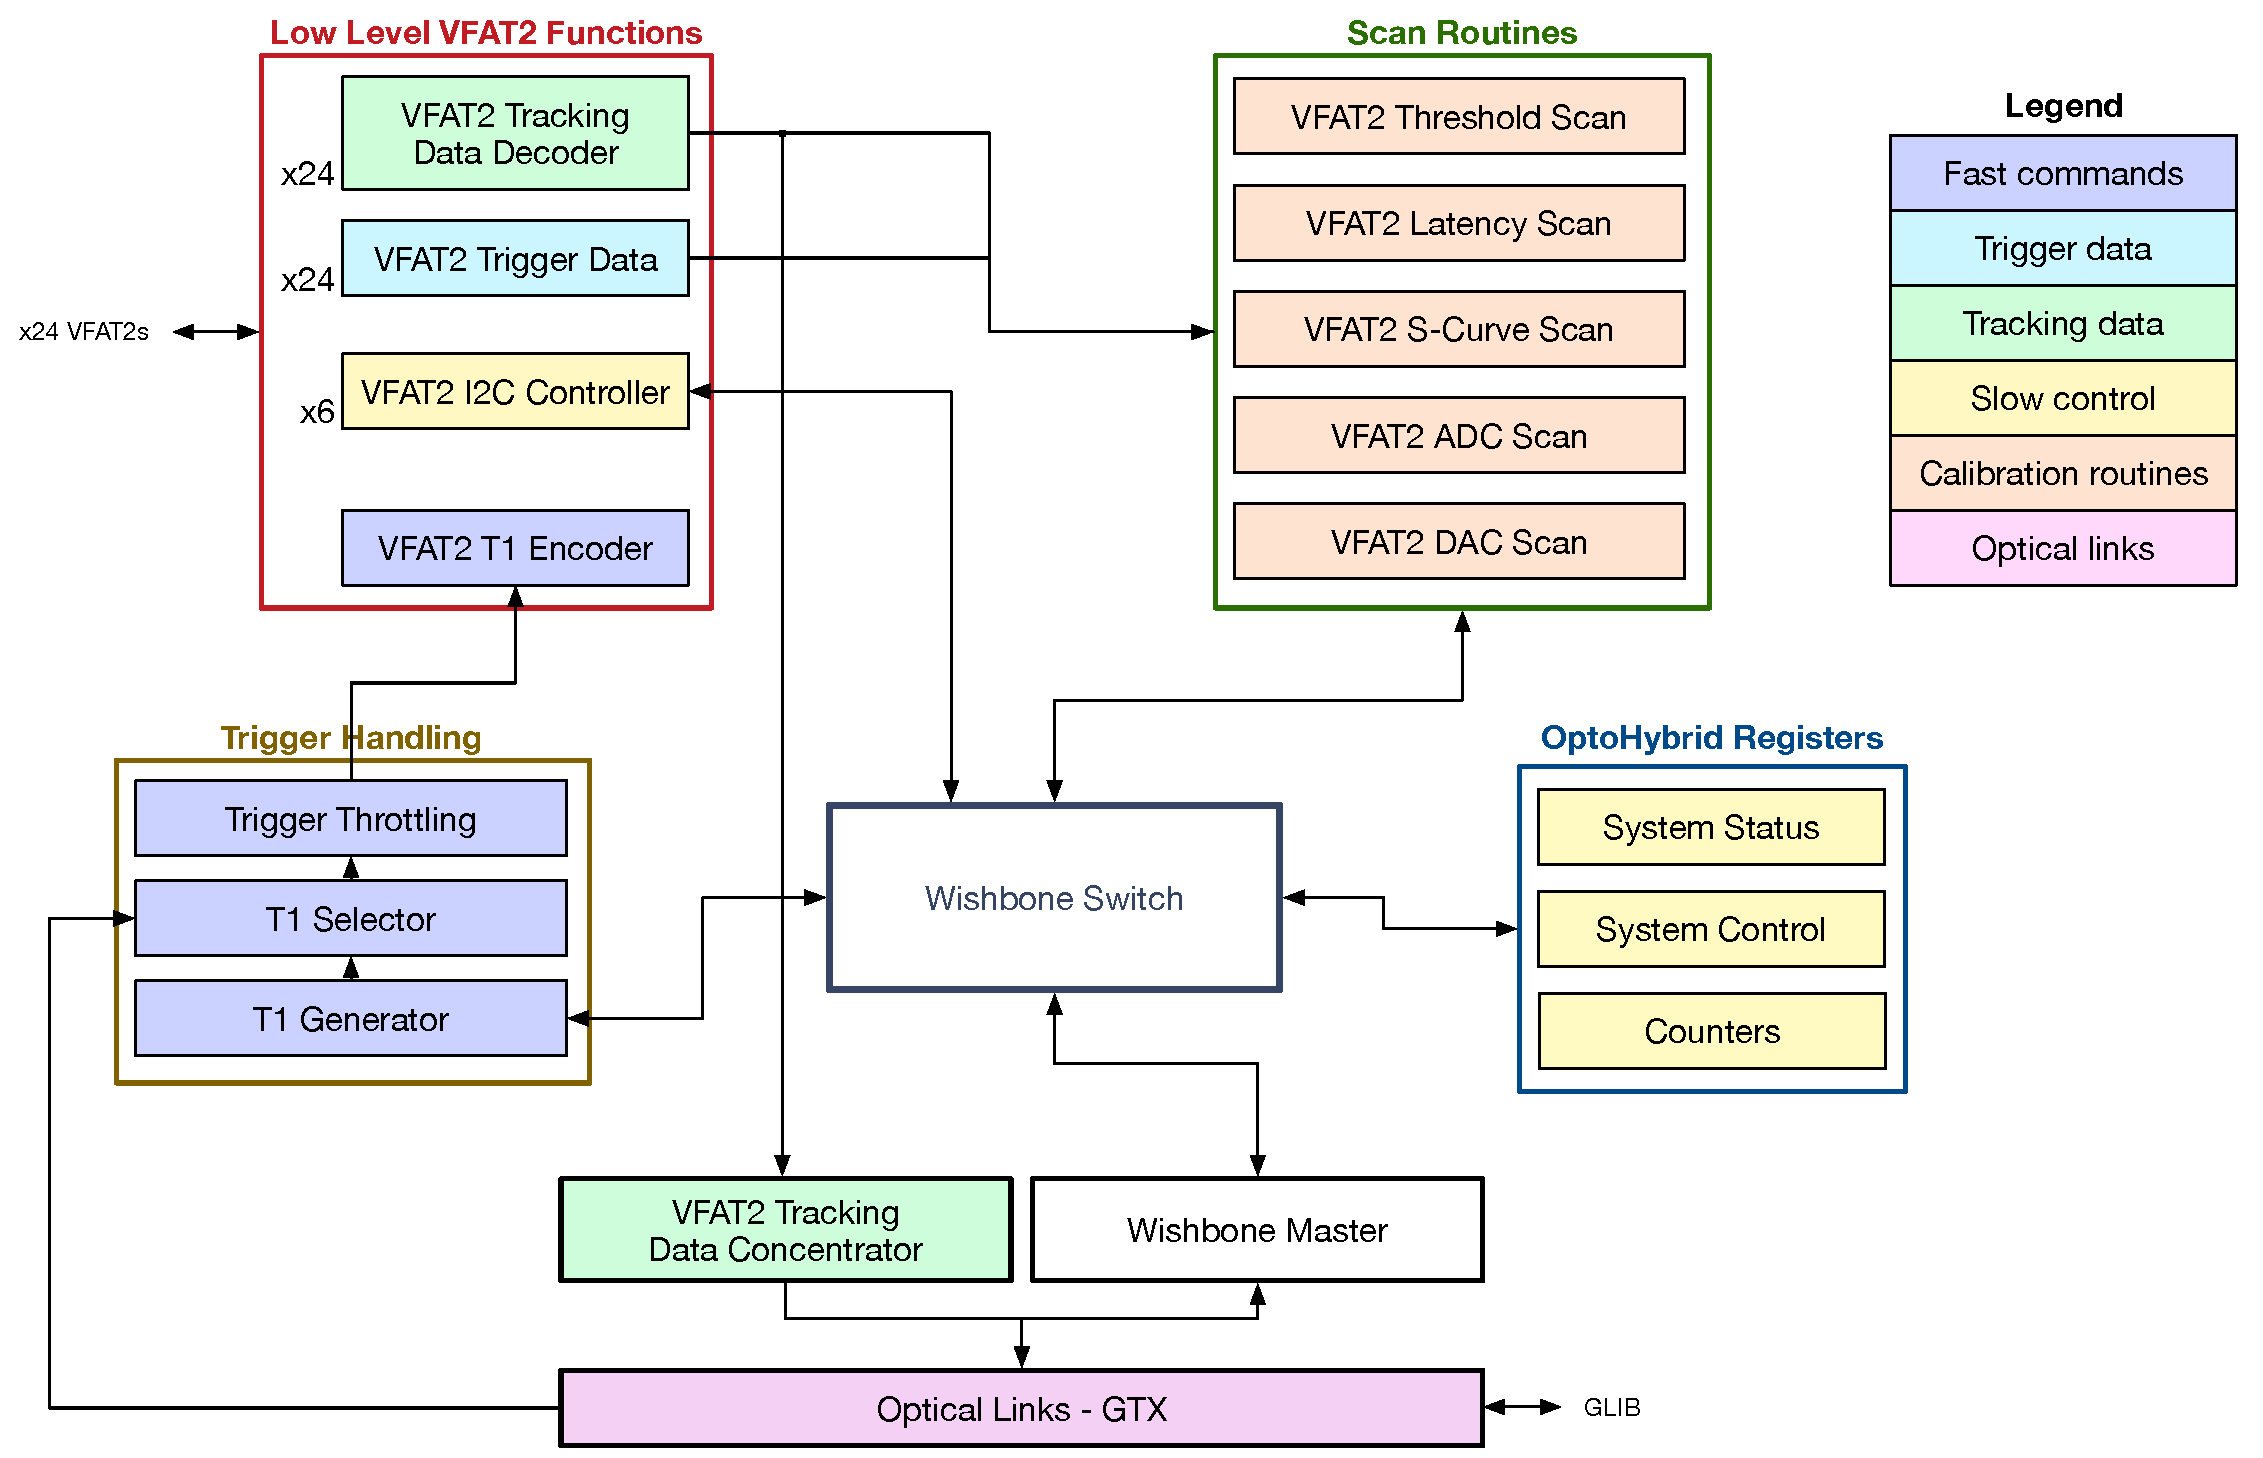
\includegraphics[width=\textwidth]{img/II-3-test-beam/system}
      \caption{Schematic diagram of the modules implemented in the firmware of the OptoHybrid regrouped by functionality.}
      \label{fig:II-3-sys}
    \end{figure}

    \subsection{Internal Communication Through a Wishbone-Like Bus}

      Wishbone is an open-source communication protocol used in many projects to enable data transfer between ICs. A light version of the protocol has been implemented in the OptoHybrid to link the various modules of the system. The latter are divided in two categories: masters which initiate requests, and slaves which provide responses. The link between the two is created through a switching hub which redirects the requests to the appropriate slaves by using a 32-bit-long address space mapped to the various modules. Some components implement both a master and a slave module in order to be able to receive requests and propagate them to various other modules. Figure \ref{fig:II-3-wishbone-arch} is a schematic illustration of the architecture of the system without Wishbone on the left and with Wishbone on the right. In the architecture of the first version of the firmware, all requests had to originate from the software routines which were the only masters of the system. This meant that the firmware modules could not communicate among themselves. In the second version, firmware routines can be developed which act as masters in the system and have direct access to all resources of the FPGA in a unified way. The right part of the figure shows how the software sends a request to the firmware routine in red, and how the firmware routine then handles the communication with the other modules. All the requests transit through the switch and are redirected to the appropriate slaves. \\

      \begin{figure}[t!]
        \centering
        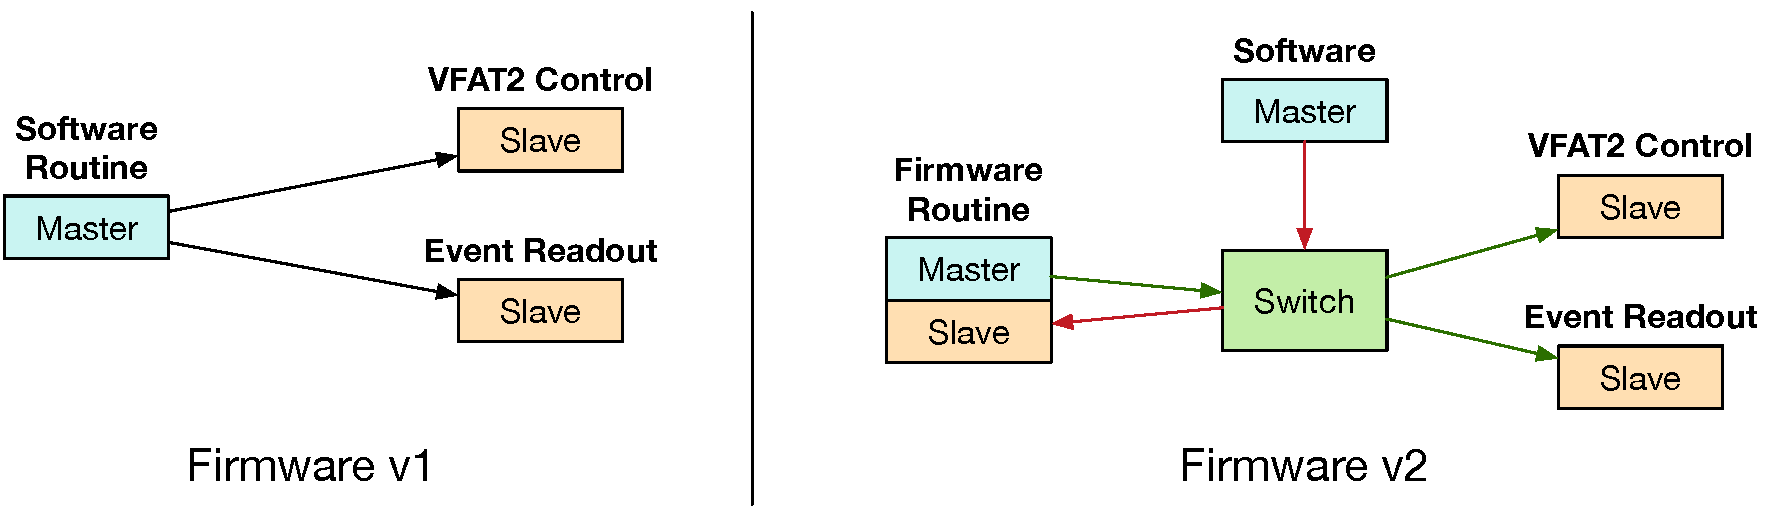
\includegraphics[width=\textwidth]{img/II-3-test-beam/wishbone_arch}
        \caption{Schematic illustration of the architecture of the system without Wishbone on the left and with Wishbone on the right.}
        \label{fig:II-3-wishbone-arch}
      \end{figure}

      To highlight the benefits of the implementation of the Wishbone-like bus on the architecture, Figure \ref{fig:II-3-wishbone-flow} presents the flow of operations for a custom calibration routine performed on the system without Wishbone on the left and with Wishbone on the right. The IPBus requests that the system has to perform are highlighted in blue, the I2C requests in orange, and the computations in green. In the system on the left, the software has to perform an IPBus request for every single action it needs to perform. Each request is sent over the network and has thus a large latency, higher than 100 ms. For complex routines, this can add up to several minutes and thus block the system. In the architecture of the second version of the firmware, the OptoHybrid itself handles the operations with the VFAT2. A single IPBus request is sent from the software to start the scan and all other operations are done in parallel by the firmware. The analysis of the data is done directly upon reception of an event and the results are stored in memory. Meanwhile, other operations can be performed by the software on the system. At the end of the scan, the software can collect the results and display them directly. \\

      \begin{figure}[b!]
        \centering
        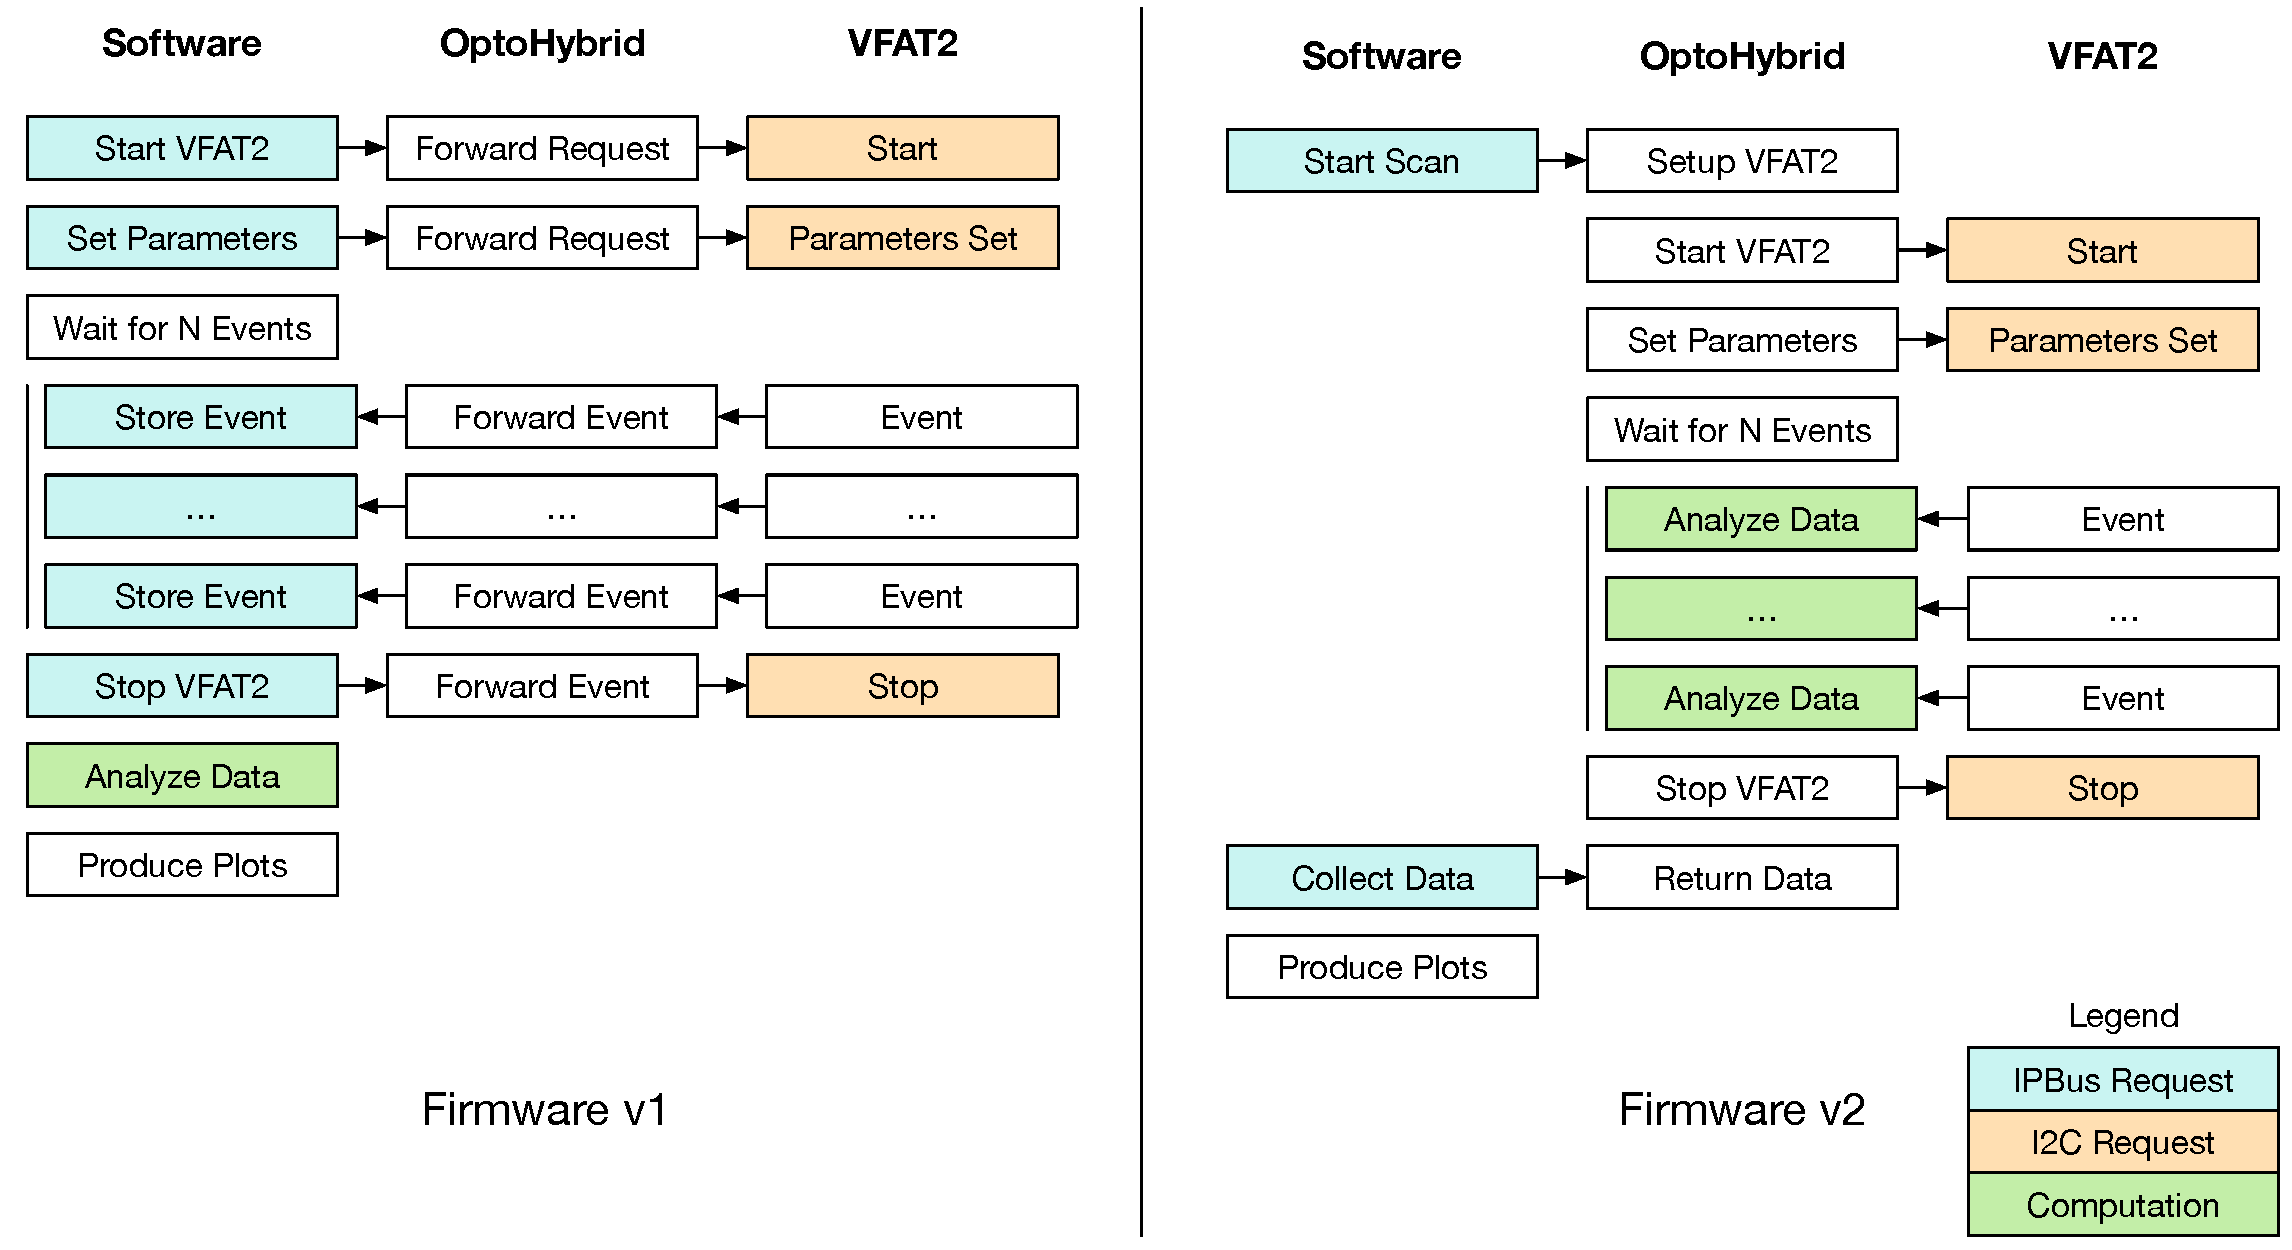
\includegraphics[width=\textwidth]{img/II-3-test-beam/wishbone_flow}
        \caption{Flow of operations for a custom calibration routine performed on the system without Wishbone on the left and with Wishbone on the right.}
        \label{fig:II-3-wishbone-flow}
      \end{figure}

      A request from a master is composed of four signals: a flag signaling the presence of a request, a write-enable bit to indicate the nature of the request (read or write), a 32-bit-long address to which the request will be redirected, and an optional 32-bit-long data field in case the request is a write operation. The response from a slave consists of: an acknowledgment signal, a 4-bit-long error status in case the operation failed, and an optional 32-bit-long data field holding the response to read requests. Figure \ref{fig:II-3-wishbone-chrono} represents a chronograph of two wishbone communications between a master and a slave for a successful write operation and a read operation resulting in an error. A programmable timeout has also been implemented to avoid blocking operation.  \\

      \begin{figure}[t!]
        \centering
        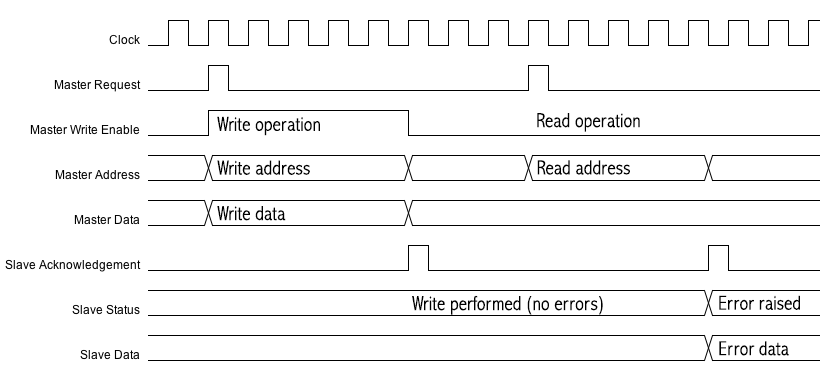
\includegraphics[width=\textwidth]{img/II-3-test-beam/wishbone-chrono.png}
        \caption{Chronograph of two wishbone communications between a master and a slave for a successful write operation and a read operation resulting in an error.}
        \label{fig:II-3-wishbone-chrono}
      \end{figure}

      Communication done through the wishbone-like protocol is used mainly for slow control or non-time-critical operations as the latency of a transactions is not fixed. Indeed, the switching hub implements a waiting list functionality, which allows two masters to address the same slave at the same time by storing one of the requests in memory and awaiting for the slave to finish the other transaction.

    \subsection{Encoding Fast Commands}

      Fast commands such as L1As, Resyncs, BC0s, etc can originate from various sources. In normal data taking runs, the AMC13 receives the TTC signals common to CMS, forwards them to the microTCA AMC which in turn transmits them to the OptoHybrid. When data taking is stopped and calibration runs are performed, the routines implemented in the OptoHybrid are run and require fast commands. To this end, the TTC signals can also be generated locally using the T1 generator module. This entity can generate L1As, Resyncs, BC0s, and CalPulses in three different ways: send a single command a given number of times at fixed interval, send a CalPulse followed by a L1A with a fixed delay, or send a programmable pattern involving all the commands. Figure \ref{fig:II-3-t1-chrono} illustrates those functionalities through a chronograph of two events generated by the T1 generator and encoded on the T1 lines for the VFAT2s: first two L1As (blue) are sent with a fixed interval, then a CalPulse (red) is generated followed by a L1A (green) after a defined delay. The T1 commands are then encoded on three bits for the VFAT2s (100 for L1As and 111 for CalPulses). \\

      \begin{figure}[t!]
        \centering
        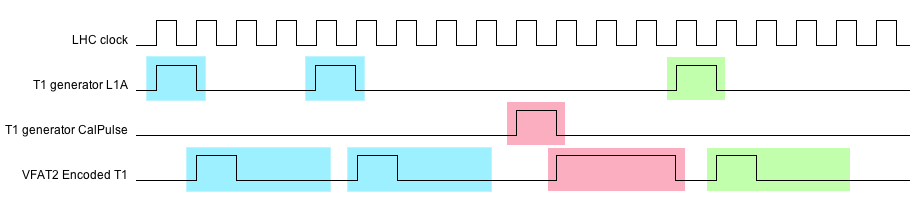
\includegraphics[width=\textwidth]{img/II-3-test-beam/t1-chrono.png}
        \caption{Chronograph of two events generated by the T1 generator and encoded on the T1 lines for the VFAT2s: first two L1As (blue) are sent with a fixed interval, then a CalPulse (red) is generated followed by a L1A (green) after a defined delay. The T1 commands are encoded on three bits for the VFAT2s ("100" for L1As and "111" for CalPulses).}
        \label{fig:II-3-t1-chrono}
      \end{figure}

      The two remaining sources of TTC commands, and more precisely L1As, are either a loopback from a given VFAT2 trigger bits directly to all the VFAT2s (self-triggering) or the signals coming from an external component through a debugging header on the OptoHybrid. The former can be used to trigger on noise or when no other source of triggers is available; the latter has been used during the test beams in conjunction with scintillators. The switching between the various sources is done by setting a register through slow control operations. Once the source has been selected, the commands are forwarded to the VFAT2s and encoded on the T1 signals. Each command is composed of three bits clocked at 40 MHz. An additional feature has been added to the L1A line to throttle the trigger signals when working in high rate environments. Through registers, the operator can select to send only a fraction of the received commands not to overload the VFAT2 buffers and allow for correct readout of the chip. Figure \ref{fig:II-3-t1-switch} summarizes the encoding of fast commands through a diagram of the switching and throttling process for T1 commands highlighting the various sources of T1 commands (blue) and the involved modules (green) before the signal is sent to the VFAT2 chips (orange).

      \begin{figure}[h!]
        \centering
        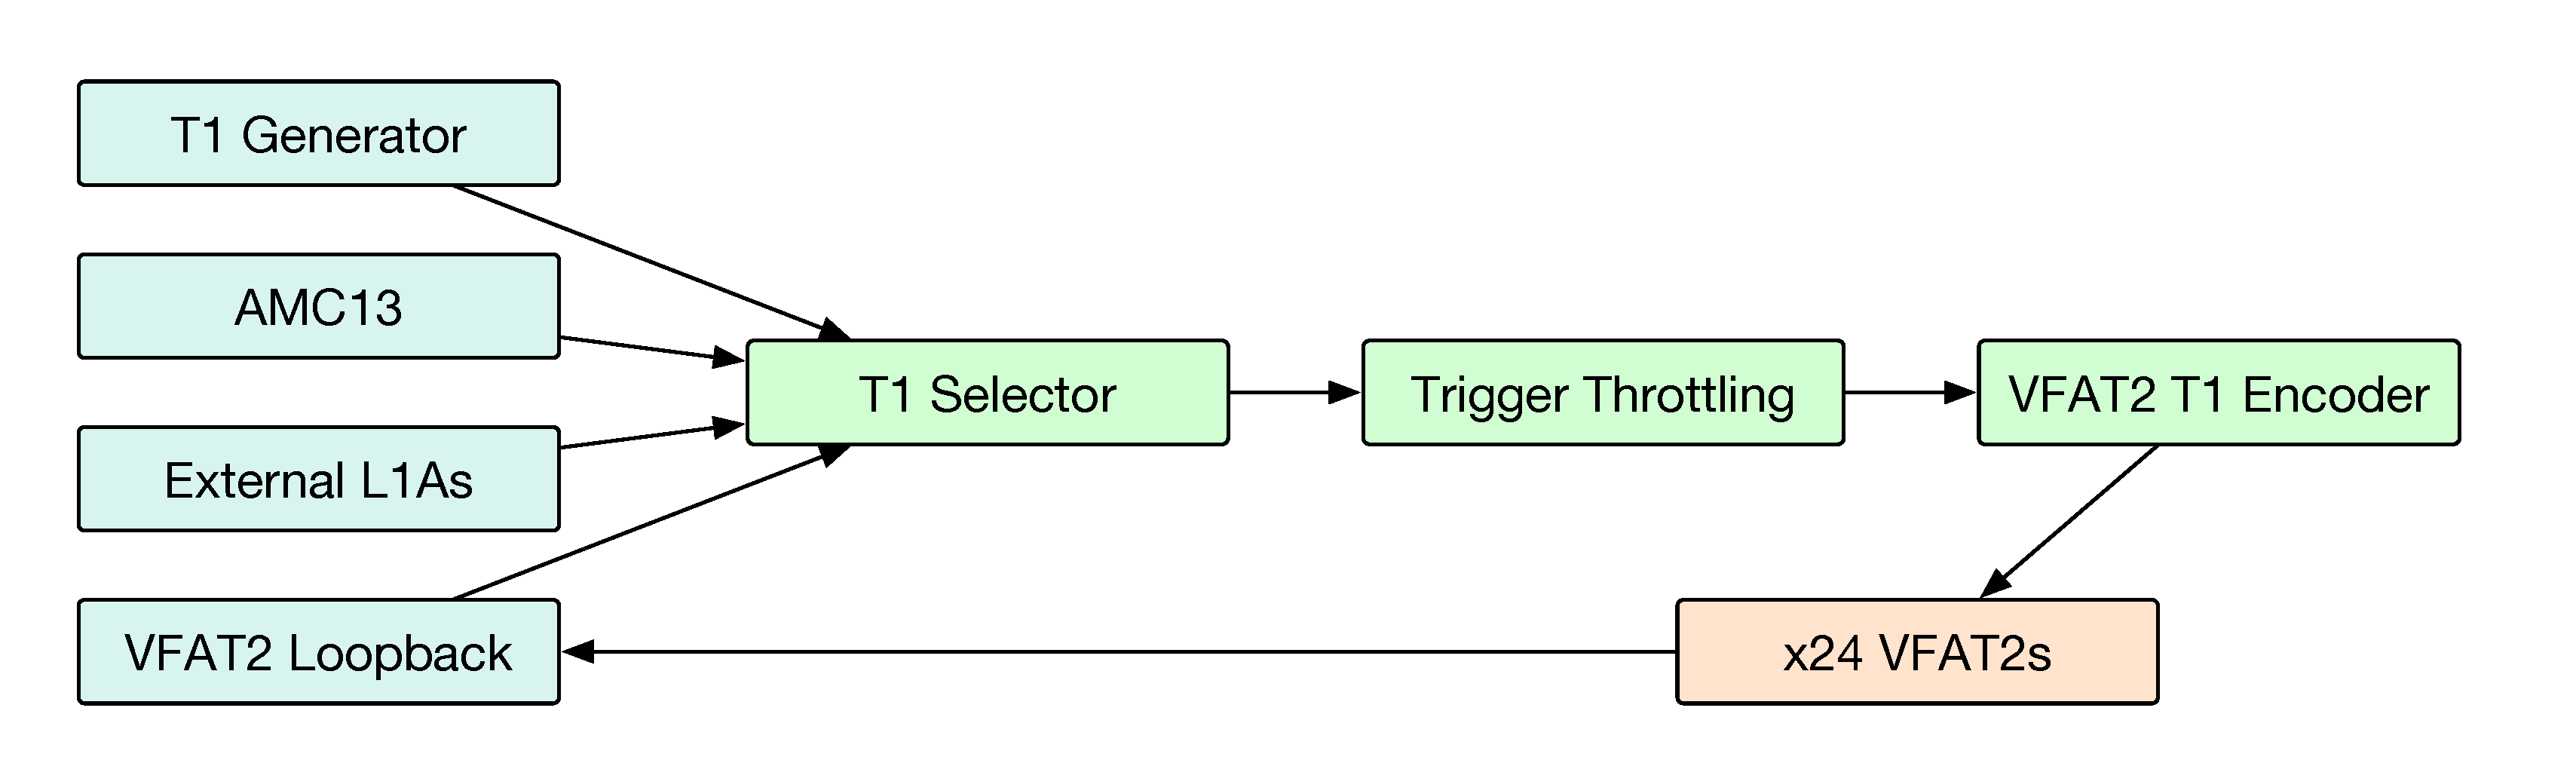
\includegraphics[width=\textwidth]{img/II-3-test-beam/t1-switch}
        \caption{Diagram of the switching and throttling process for T1 commands highlighting the various sources of T1 commands (blue) and the involved modules (green) before the signal is sent to the VFAT2 chips (orange).}
        \label{fig:II-3-t1-switch}
      \end{figure}

    \subsection{Formatting Trigger Data}

      Each of the 24 VFAT2s transmits eight trigger bits per BX. These are regrouped using a logic OR in the firmware of the OptoHybrid thus yielding 24 bits. The trigger information is used for calibration routines and forwarded over debugging headers to an external electronics crate. As the number of external connections is limited, only six trigger bits can be sent, thus requiring the need for a selection mechanism controlled by programmable registers.

    \subsection{Acquiring Tracking Data}

      Upon reception of a L1A, the VFAT2 transfers the selected event from its SRAM1 to SRAM2 and then to an encoder which serializes the data. Each event is 192 bits long followed by two idle bits and clocked at 40 MHz. This means that it takes 194 BXs to read out one event and that the VFAT2 cannot handle trigger rates higher than $\approx$ 200 kHz without experiencing an overflow of the buffers. The data is pushed out of the VFAT2 automatically and formatted according to the pattern shown in Table \ref{tab:II-3-vfat2-tk-format}. The top left bits are the Most Significant Bits (MSBs) which are pushed out first and the bottom right bits or the Least Significant Bits (LSBs) which come in last. The first four bits of the first three 16-bit-long words are constant values. These are completed by the BC which increments at each clock cycle, the EC which counts the number of received L1As, four flags which hold information on the status of the buffers, and a chip ID unique to each VFAT2. Following are the 128 bits reflecting the hit information on each channel. Finally, the VFAT2 uses a Cyclic Redundancy Check (CRC) on 16 bits to detect errors. The CRC uses all other 176 bits to encode its data but does not provide a way to correct errors. \\

      \begin{table}[h!]
        \begin{tabularx}{\textwidth}{C{1}}
          \textbf{VFAT2 tracking data} \\
          { \small
          \begin{tabularx}{0.5\textwidth}{|C{1}|C{1}|C{1}|}
            \hline
            \multicolumn{3}{|c|}{15 \hfill 0} \\ \hline
            1010 & \multicolumn{2}{|c|}{BC[11:0]} \\ \hline
            1100 & EC[7:0] & Flags[3:0] \\ \hline
            1110 & \multicolumn{2}{|c|}{Chip ID[11:0]} \\ \hline
            \multicolumn{3}{|c|}{Channel data x8} \\ \hline
            \multicolumn{3}{|c|}{CRC} \\ \hline
          \end{tabularx} }
        \end{tabularx}
        \caption{Format of the tracking data packets sent by the VFAT2s.}
        \label{tab:II-3-vfat2-tk-format}
      \end{table}

      Next to the data line, each VFAT2 provides a DataValid line which is pulled high when the bits exiting the VFAT2 are valid. However, due to the limited number of pins connecting the GEB and the OptoHybrid, this signal has been left unconnected for all but six VFAT2s. Therefore, data is constantly shifted in a 194 bits (192 bits of data and 2 idle bits) serial-to-parallel converter and analyzed. When the fixed pattern of 12 bits is seen, a flag is raised signaling the presence of potential data. The data packet is split up in its various elements and the CRC is recomputed and compared against the received CRC. Two additional flags respectively hold the results of the comparison of both CRCs indicating if the data is valid or not, and a logic OR of all 128 channel to indicate if the packet contains a hit or not. Figure \ref{fig:II-3-tkdata-chrono} illustrates this process through a chronograph of the serial decoding of an incoming data packet (blue) which is analyzed and placed in parallel busses (yellow) with the CRC check bit and the hit present bit. In theory, only packets with valid CRCs could be transmitted to the back-end electronics. However, sending all packets offers the possibility to identify recurring errors in the CRCs computation and the possibility to correct them offline. To this end, a programmable register is used to select whether packets with a corrupted CRC should be sent or not. \\

      \begin{figure}[h!]
        \centering
        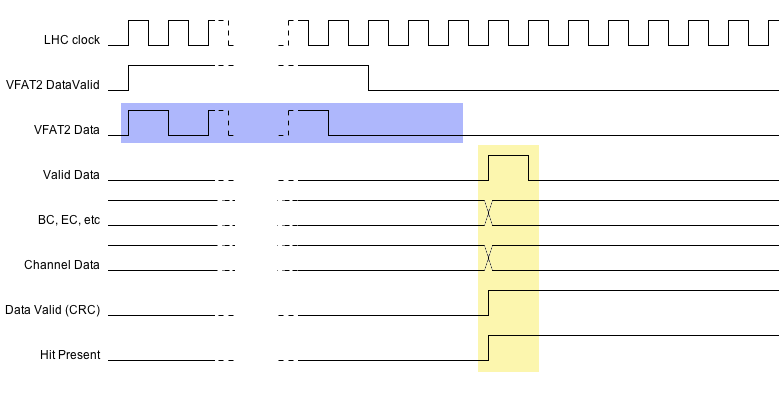
\includegraphics[width=\textwidth]{img/II-3-test-beam/tkdata-chrono.png}
        \caption{Chronograph of the serial decoding of an incoming data packet (blue) which is analyzed and placed in parallel busses (yellow) with the CRC check bit and the hit present bit.}
        \label{fig:II-3-tkdata-chrono}
      \end{figure}

      In parallel to the decoding of the data packets, the OptoHybrid maintains its own BC and EC and stores the value of the counters in a buffer each time a L1A is received. When the 24 decoding modules, one for each VFAT2, report they have detected data, a concentrator module aggregates the information from all available VFAT2s. Every packet received within a window of ten BX is assigned to the same event to which the value of the corresponding BC and EC is appended. The assembled event is stored in a large buffer to be later sent over the optical links to the GLIB. Additionnaly, the data decoder can perform zero suppression on the packets, suppressing them when no strips have been hit in the event. \\

      To prevent positions either not equipped with VFAT2 Hybrids or that are noisy to generate fake data, a 24-bit-long register allows the masking of individual positions to ignore any packets it generates. Next to this, each decoding module is equipped with two counters respectively counting the number of valid and invalid packets.

    \subsection{Controlling and Monitoring the Systems}

      The OptoHybrid is used to control itself through wishbone and the VFAT2s through I2C \cite{i2c}. The slow control of the OptoHybrid mainly consists in selecting TTC command sources, setting the trigger throttling, reading out counters, etc. These operations are performed to control the data flow and the functioning of the DAQ system itself. Commands sent to the VFAT2s on the other hand have direct impact on the physics of the data taking through the bias of the analog front-end readout. \\

      The I2C protocol uses two signals to connect one master to multiple slaves: one clock (SCK) and one data (SDA) line. The master controls the clock signal which defines the reference clock of the exchanges. The data line on the other hand is driven by both the master and the slaves according to a defined data format. The official I2C data frame is shown in Figure \ref{fig:II-3-i2c}. A communication is always started by the master by driving SDA low when SCK is high. The master then sends seven address bits (yellow) which are used to identify the slave it wants to talk to, followed by a read/write bit (R/W, blue). If a slave was configured to respond to the address, it will drive SDA low to signal an acknowledgement (ACK, green). Afterwards, eight bits (red) are sent from the master to the slave in case of a write operation followed by a slave acknowledgment (ACK, green), or the opposite in case of a read operation. The frame ends when the master drives SDA high while SCK is low. \\

      \begin{figure}[h!]
        \centering
        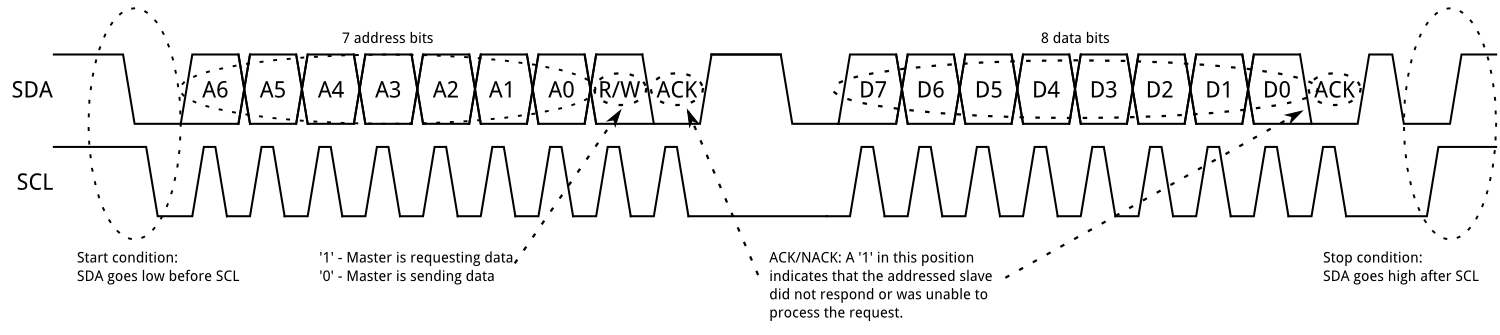
\includegraphics[width=\textwidth]{img/II-3-test-beam/i2c.png}
        \caption{Chronograph of an I2C communication.}
        \label{fig:II-3-i2c}
      \end{figure}

      To communicate with the VFAT2s, six I2C controllers are implemented in the firmware of the OptoHybrid, one per sector on the GEB. Each controller can access four VFAT2s which are identified using three resistors that can be installed on the GEB. VFAT2 uses a modified I2C protocol with the same frame format as the official one, but a different addressing scheme. For the VFAT2, the first three bits of the address are used to select the chip that is addressed by the master while the four remaining bits are used to select the register that needs to be accessed. This addressing scheme allows the OptoHybrid to access up to 16 registers on the VFAT2s. Figure \ref{fig:II-3-i2c-vfat2} represents a chronograph of the modified I2C communication for the VFAT2. \\

      \begin{figure}[h!]
        \centering
        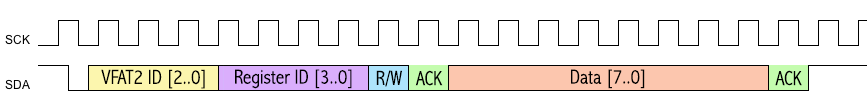
\includegraphics[width=\textwidth]{img/II-3-test-beam/i2c-vfat2.png}
        \caption{Chronograph of an I2C communication performed with the VFAT2.}
        \label{fig:II-3-i2c-vfat2}
      \end{figure}

      However, each VFAT2 holds 16 primary registers and 136 extended registers. The latter are accesses using two primary registers: one set to point to an extended register (Extended Pointer), and one to read/write the data in said register (Extended Data). Thus, in order to perform a transaction on a primary register, only one operation is necessary, while two are required to access extended registers. A first operation will modify the content of the Extended Pointer register to point to the desired extended register, and a second operation will read/write the Extended Data register to affect the extended register. Figure \ref{fig:II-3-i2c-extended} illustrates how the extended registers are addressed through two primary registers. \\

      \begin{figure}[h!]
        \centering
        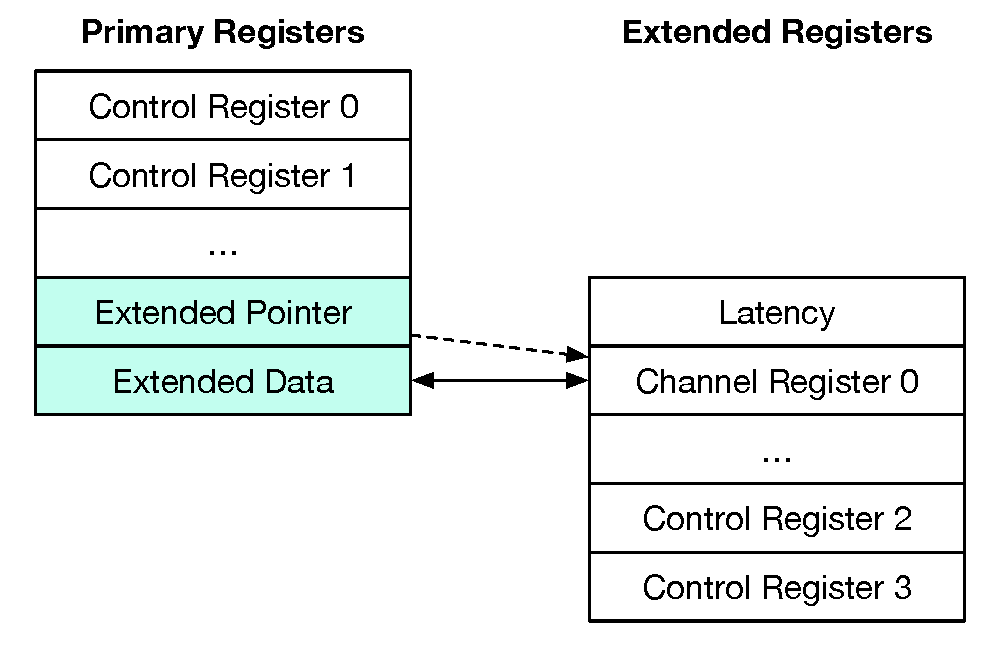
\includegraphics[width=0.6\textwidth]{img/II-3-test-beam/i2c-extended}
        \caption{Addressing of the extended registers through two primary registers.}
        \label{fig:II-3-i2c-extended}
      \end{figure}

      To make this process transparent to the user and flatten out the address space of the VFAT2s, the OptoHybrid maps the primary registers from addresses 0 to 15 and the extended registers from addresses 16 to 151. When performing a transaction with the extended registers, the I2C controllers automatically run the double addressing scheme. \\

      Next to the basic I2C controllers, an extended I2C controller was developed to abstract individual addressing and allow request broadcasting. This module forwards I2C requests to all selected VFAT2s at once to configure the entire system in parallel. A programmable register makes it possible to leave out given VFAT2s from the broadcast while a buffer stores the result of the operations.

    \subsection{Calibrating the Systems}

      The calibration routines have been ported from software to firmware in order to increase their speed of operation and reduce the number of requests that need to be performed. The routines are as follows: a threshold scan which measures the noise on the channels as a function of the threshold of the VFAT2s; a latency scan which allows to select the correct BX when receiving L1As; a s-curve scan which characterize the response of the channels as a function of the collected charge and threshold; an analog-to-digital converter (ADC) scan which reads out the information from the ADC embedded in the FPGA; and a digital-to-analog converter (DAC) scan which is used to convert information stored in the VFAT2 registers to voltages and currents. Two versions of the scans exist: one which performs the scans on a single VFAT2, and one which is able to run on multiple VFAT2s in parallel using a mask to define which ones it should target. The latter improves the speed by a factor of 24 compared to the former when performing systematic scans on the entire detector.

      \paragraph{The threshold scan} is used to scan each VFAT2 for noise. For each threshold value set on the VFAT2, the percentage of events displaying a hit is recorded and taken as the percentage of noise. A graph, as depicted in Figure \ref{fig:II-3-threshold-scan}, can be obtained showing the noise decrease as the threshold increases yielding a point at which the system can be operated with minimal noise. The threshold scan can be operated at the chip level using trigger information or the 128 channels as a whole, or on individual channels using tracking data. For the latter, the T1 generator is used as trigger source to generate data as these runs are being performed when the beam is off. No relation between a L1A and physical event is needed to study the noise on the system.

      \begin{figure}[h!]
        \centering
        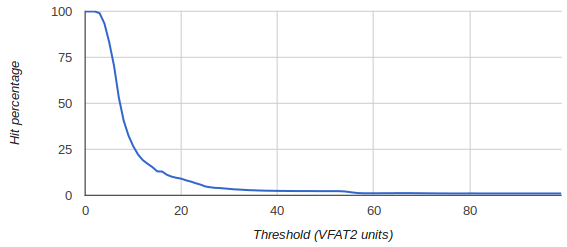
\includegraphics[width=0.7\textwidth]{img/II-3-test-beam/threshold_scan.png}
        \caption{Illustration of a threshold scan representing the hit percentage as a function of the threshold of the VFAT2.}
        \label{fig:II-3-threshold-scan}
      \end{figure}

      \paragraph{The latency scan} allows to determine the best latency value to be set in a VFAT2. The latency is the time difference, in number of BX, between the time of arrival of a L1A and the time at which the related event was stored in the VFAT2 buffer. This module is operated when the particle beam is on and triggers are generated by an external source such as a Photomultiplier (PM) placed in front of the detector. For each value of the latency, the OptoHybrid counts the ratio of events with hits over the total number of events. Figure \ref{fig:II-3-latency-scan} is an illustration of an ideal latency scan representing the hit percentage as a function of the latency of the VFAT2. For a noiseless VFAT2 with 100\% detection efficiency, the ratio would be 0\% outside the correct latency window and 100\% inside. The size of the window can be adjusted by changing the length of the output of the monostables in the VFAT2s.

      \begin{figure}[h!]
        \centering
        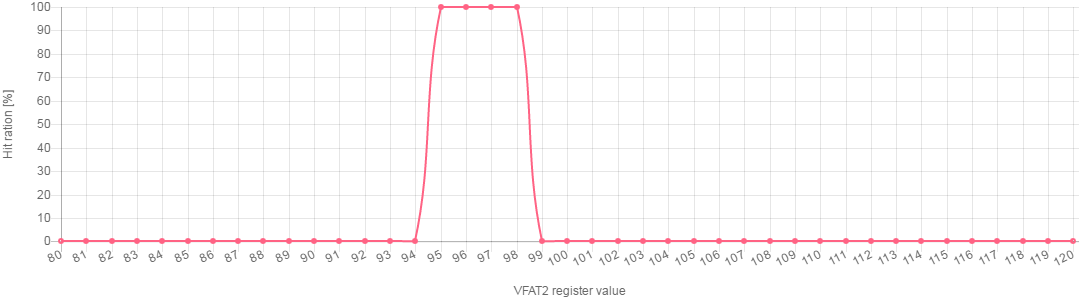
\includegraphics[width=0.7\textwidth]{img/II-3-test-beam/latency_scan.png}
        \caption{Illustration of an ideal latency scan representing the hit percentage as a function of the latency of the VFAT2.}
        \label{fig:II-3-latency-scan}
      \end{figure}

      \paragraph{The s-curve scan} is part of the calibration routines performed for the qualification of the VFAT2s. It yields the response of the VFAT2 channels to an injected charge pulse according to the threshold. It is used in conjunction with the T1 generator which sends a CalPulse followed by a L1A at fixed interval, thus with known latency. The use and results obtained for this module are further detailed in Chapter \ref{chap:II-4-qualification}.

      \paragraph{The ADC scan} reads out the ADC embedded inside the fabric of the FPGA of the OptoHybrid. The Xilinx Virtex-6 FPGAs embark a system monitor \cite{VIRTEX-SYSMON} which offers the possibility to convert voltages to ADC counts with a resolution of 10 bits over 1 V, resulting in a precision of 977 $\mu$V. The inputs of the ADC are connected to voltage lines of the OptoHybrid and to analog signals coming from the VFAT2s.

      \paragraph{The DAC scan} is used to characterize the analog front-end of the VFAT2s. When a digital value is written in given registers of the VFAT2, it is converted to a voltage or current in the amplification and shaping stages of the electronics. These can optionally be driven out of the VFAT2 for monitoring and be connected to the ADC of the OptoHybrid. The DAC scan provides a routine which associates every value written in the registers of the VFAT2s and the corresponding ADC counts, and thus voltage or current.

    \subsection{Optical Communication with the Off-Detector Electronics}

      The connection between the OptoHybrid and the off-detector electronics is the optical links from which two are used: one for the trigger data and fast commands, and one for the tracking data and slow control. Each optical fiber is connected to an SFP+ transceiver which contains the Light Emitting Diode (LED) that drives the link. The SFP+ module is in turn connected to a Gigabit Transceiver X (GTX) block inside the FPGA, which is a dedicated component that can handle high-speed serial communications.

      \paragraph{The GTX module} is in charge of the serialization/deserialization of high-speed data up to 6.6 Gbps. A schematic diagram of the functions it provides is shown in Figure \ref{fig:II-3-gtx}. The GTX handles both the transmission and reception of data. From the FPGA logic, it receives a parallel vector of bits containing the raw data. The raw data enters the Transmit FIFO which acts as a buffer before the Line Encoding module. The latter uses an eight-bit/ten-bit (8b/10b) encoding scheming which is a standard in high-speed communications. 8b/10b encodes every eight bit word on ten bits according to a predefined table. It has the particularity that whatever combination of words might be sent, no more than five successive '0's or '1's will arise in the serial stream. This ensures line balancing: the fact that the electric lines between the GTX and the SFP+ module will remain at an average voltage and not drift to a logic '1' or '0' over time, thus requiring a longer fall or rise time of the signals. 8b/10b also offers a set of K-characters which are unique patterns of bit that can never arise randomly in the stream. Those characters are used to detect the beginning of a frame and allow the receiver to align correctly. Finally, after the encoding of the data frame is done, it is serialized and transmitted to the SFP+ module over differential pairs. \\

      \begin{figure}[t!]
        \centering
        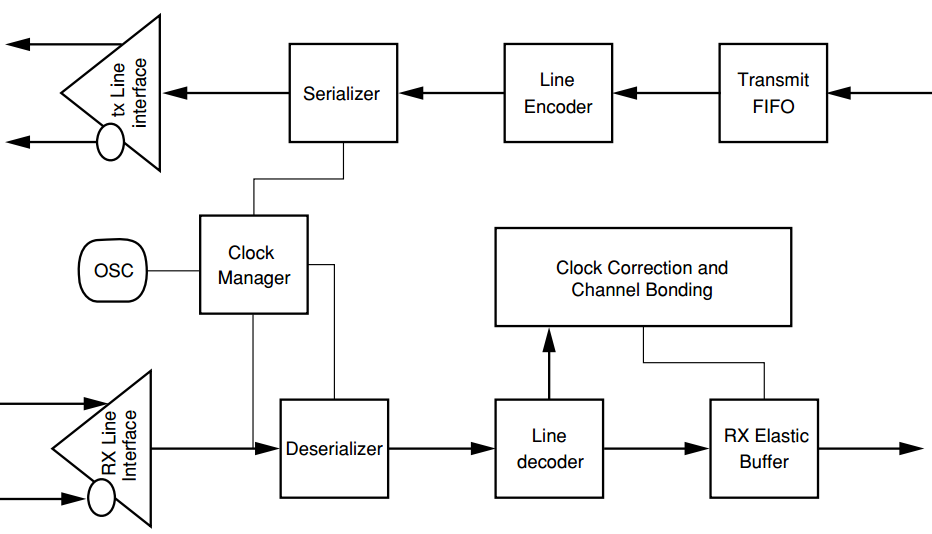
\includegraphics[width=0.8\textwidth]{img/II-3-test-beam/gtx.png}
        \caption{Functionnal diagram of the Gigabit Transceiver X module used inside the Xilinx Virtex-6 FPGAs for high-speed serial communication \cite{GTX}.}
        \label{fig:II-3-gtx}
      \end{figure}

      The receiver essentially follows the opposite path as the transmitter except for the Clock Management block. The 8b/10b encoding offers one more advantage which is the possibility to recover a clock from the data stream itself, technique called Clock Data Recovery (CDR). In high-speed signal design, small variations in the clock frequency between the transmitter and the receiver can lead to discrepancy in the read out data. To avoid this, the receiver can tune the frequency of the clock of its deserializer using the transitions of the bits in the incoming stream to align its phase to the data. The GTX block further provides the obtained recovered clock to the FPGA to use in the logic. Correct alignment of the data is checked using the K-characters in the stream.

      \paragraph{The fixed latency link} is used to transmit trigger data from the OptoHybrid to the GLIB and receive the fast commands at a speed of 3.2 Gbps. The data format used to communicate between the on-detector and off-detector electronics is detailed in Table \ref{tab:II-3-trigger-format}. Of the 64 bits that the downlink transmits every BX, 16 are used to align the serial bit stream on the receiving side through a header and four others are used to encode the four fast commands that the VFAT2 understands. The other 44 bits are not used and left to constant zeros. The uplink uses a 16 bit header to align the stream to which it appends 24 bits, one bit per VFAT2 corresponding to the logic-OR of its trigger bits. These patterns repeat at 40 MHz as data changes every BX.

      \begin{table}[h!]
        \begin{tabularx}{\textwidth}{C{1}C{1}}
          \multicolumn{2}{c}{\textbf{Fixed latency link}} \\
          \textbf{GLIB to OptoHybrid frame} & \textbf{OptoHybrid to GLIB frame} \\
          { \small
          \begin{tabularx}{0.4\textwidth}{|C{1}|C{1}|}
            \hline
            \multicolumn{2}{|c|}{15 \hfill 0} \\ \hline
            \multicolumn{2}{|c|}{Header} \\ \hline
            TTC[3:0] & Unused[11:0] \\ \hline
            \multicolumn{2}{|c|}{Unused} \\ \hline
            \multicolumn{2}{|c|}{Unused} \\ \hline
          \end{tabularx} }
          &
          { \small
          \begin{tabularx}{0.4\textwidth}{|C{1}|C{1}|}
            \hline
            \multicolumn{2}{|c|}{15 \hfill 0} \\ \hline
            \multicolumn{2}{|c|}{Header} \\ \hline
            \multicolumn{2}{|c|}{Trigger data[15:0]} \\ \hline
            Trigger Data[7:0] & Unused[7:0] \\ \hline
            \multicolumn{2}{|c|}{Unused} \\ \hline
          \end{tabularx} }
        \end{tabularx}
        \caption{Format of the data packets used to communicate between the GLIB and OptoHybrid on the fixed latency link.}
        \label{tab:II-3-trigger-format}
      \end{table}

      \paragraph{The variable latency link} is used to transmit and receive slow control commands and to transmit the tracking data of one VFAT2 at the time to the GLIB. As only one VFAT2 was exposed to the beam at any given time during the test beam, reconstructing and sending the full event from the 24 VFAT2s was not a necessity for the DAQ system. The format used to transmit the data is detailed in Table \ref{tab:II-3-data-format}. In both directions, a given frame format is constantly sent using two bits in the header to indicate the presence of a valid slow control request and valid VFAT2 tracking data in case of the uplink. Both send a 16 bit header to align the link followed by the frame data. As can be seen in the table on the left, the OptoHybrid receives requests from the optical link which are then converted to wishbone-like requests by the logic. The optical link module is one of the wishbone masters that controls the system and whose responses are forwarded back to the GLIB.

      \begin{table}[h!]
        \begin{tabularx}{\textwidth}{C{1}C{1}}
          \multicolumn{2}{c}{\textbf{Variable latency link}} \\
          \textbf{GLIB to OptoHybrid frame} & \textbf{OptoHybrid to GLIB frame} \\
          { \small
          \begin{tabularx}{0.4\textwidth}{|C{1}|}
            \hline
            15 \hfill 0 \\ \hline
            Header \\ \hline
            Request address (MSB) \\ \hline
            Request address (LSB) \\ \hline
            Request data (MSB) \\ \hline
            Request data (LSB) \\ \hline
            CRC \\ \hline
          \end{tabularx} }
          &
          { \small
          \begin{tabularx}{0.4\textwidth}{|C{1}|}
            \hline
            15 \hfill 0 \\ \hline
            Header \\ \hline
            VFAT2 data 14x 16 bits \\ \hline
            Response data (MSB) \\ \hline
            Response data (LSB) \\ \hline
            CRC \\ \hline
          \end{tabularx} }
        \end{tabularx}
        \caption{Format of the data packets used to communicate between the GLIB and OptoHybrid on the variable latency link.}
        \label{tab:II-3-data-format}
      \end{table}

    \subsection{System Summary}

      The aim of the firmware of the OptoHybrid is to provide a communication medium between the VFAT2s and the off-detector electronics and to speed up the calibration routines by implementing them closer to the detector. The developments that have been listed in this chapter are targeted at the OptoHybrid v2a and the configuration of the system ran during the test beams. Modifications have to be brought for the final system although the foundations of the firmware have been solidly laid out.

  \section{Architecture of the GLIB Firmware}

    The GLIB development group at CERN provides a system firmware which controls the on-board components, handles the communication with the MCH, and implements the logic to decode IPBus requests described in Section \ref{sec:II-2-ipbus}. This code is similar to the operating system in which the users run their applications by adding custom firmware. The latter is system specific and up to the user to develop. In this application, the firmware developed for the GLIB is in charge of the buffering of the tracking data until it is read out by the application, and the forwarding of the IPBus requests over the optical link to the OptoHybrid. In addition, the GLIB holds a couple of counters which monitor the status of the optical links and the number of requests performed. However, the firmware of the GLIB has been designed to be able to handle two OptoHybrids in parallel, seamlessly allowing the user to switch from one to another at any time.

    \subsection{The Tracking Data Readout}

      The GLIB acts as buffer for the tracking data it reads out from the OptoHybrids and decodes from the optical links. It stores the VFAT2 events until the control and monitoring application reads them out through IPBus. In case the buffers reach their full occupancy, new events are discarded and flags are raised. The buffers can hold up to 16 383 VFAT2 events per connected OptoHybrid. Additionally, the system has been tested and proven to work without overflows up until L1A rates of 200 kHz, the maximum rate the VFAT2s can handle.

    \subsection{The IPBus Controller and Slaves}

      The IPBus decoding procedure is similar to the wishbone system implemented on the OptoHybrid. According to the address contained in the request, the GLIB selects the slave it needs to address. Each request is made of a flag signaling the presence of a request, a read/write bit reporting the type of operation, a 32-bit-long address field, and an optional 32-bit-long data field populated with data in case of a write operation. The IPBus response is composed of an acknowledgment and error flag to signal the validity of a response, and an optional 32-bit-long data field containing the read data. By design, each IPBus request is decomposed in single read or write operations. Therefore, even if the software performs a read request of multiple addresses at once, IPBus slaves will still see this as multiple sequential read operations on single addresses. This in turn propagates to the OptoHybrid wishbone requests which originate from IPBus, meaning that no more than one operation coming from the GLIB is present at any time in the system. As a majority of the requests have to be forwarded to the OptoHybrid, an entire address space of the GLIB is mapped to the former. These are handled by an IPBus slave connected to the GTX blocks of the GLIB. This module encodes the request according to the data format on the left in Table \ref{tab:II-3-data-format} and awaits for a response before signaling the IPBus controller.

  \section{The Control and Monitoring Application}

    The first version of the control and monitoring application that communicated with the system was based on a series of Python scripts running PyChips, a Python implementation of IPBus provided with the GLIB source code. Each script was developed to run a specific task and needed to be run over and over again. This was feasible for the first test beam during which only the system was tested for small amounts of time, but not for the second one that was meant to collect data. Therefore, a web application was developed based on NodeJS \cite{NODEJS} as server technology, SocketIO \cite{SOCKETIO} for the client/server exchange, AngularJS \cite{ANGULARJS} as front-end framework, and Bootstrap \cite{BOOTSTRAP} as design framework. The architecture of the application is depicted in Figure \ref{fig:II-3-app-layout} which shows how the various technologies interact.

    \begin{figure}[t!]
      \centering
      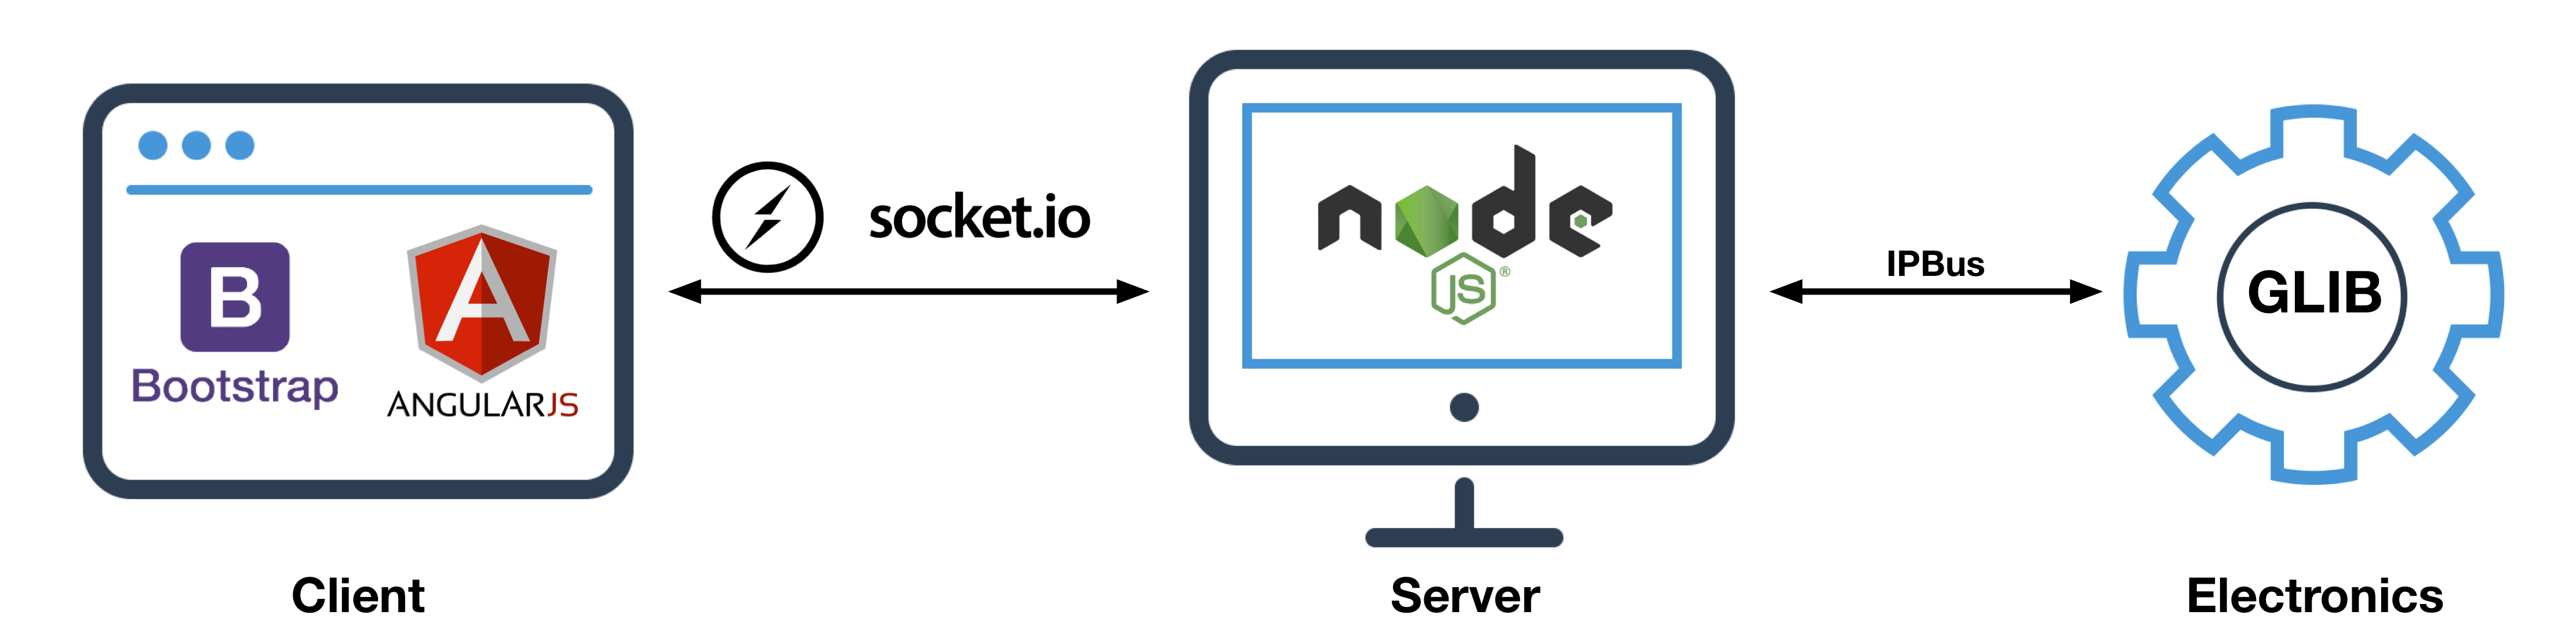
\includegraphics[width=\textwidth]{img/II-3-test-beam/app-layout.png}
      \caption{Functional diagram of the architecture of the application used to control and monitor the GEM detectors.}
      \label{fig:II-3-app-layout}
    \end{figure}

    \subsection{Architecture of the Application}

      NodeJS is a JavaScript (JS) runtime that has the ability to run JS code outside the context of a web browser. It extends JavaScript from its original use in web content to a wide range of applications by enabling it to manipulate files, data streams, etc. The most common use for NodeJS is the implementation of a web server that has the ability to be much more reactive than other infrastructures. Where classic server structures display a blocking behavior, meaning they only handle one request at a time, blocking the queue of incoming demands, NodeJS is event driven and thus non-blocking. For example, if a client requests a file, NodeJS will transfer the request to the operating system and continue to respond to other client as long as the file is not served. Interactions are thus more reactive and allow for easy implementation of a real-time control and monitoring system. Alongside the NodeJS server that serves the content of the web application, a version of IPBus in JS was also implemented. The latter allows the server to execute IPBus requests on the GLIB and readout the response. \\

      To link the client side controlled by the user and the server side which sends requests to the GLIB, the SocketIO project is used. It is an abstraction layer on the fairly new WebSocket technology which adds sockets to web browsers and allows for fast communication with servers by bypassing the HTTP protocol. When the client changes settings in its web browser, SocketIO transfers the request to NodeJS which in turn creates an IPBus packet. When the GLIB responded to the request, the server transfers the response back to the client which can handle the data as it likes. \\

      To handle data in a dynamic and convenient way, the web pages use Bootstrap and AngularJS. Bootstrap is a design framework which provides simple and readable themes to layout the pages. The content of the page on the other hand is managed by AngularJS which is a front-end JS framework. It helps render dynamic content in function of the data received from the server. Actions can be triggered or disabled according to the state of the system, data can be updated live, etc. It renders the user experience more fluid and enjoyable by providing a usable set of actions and an efficient navigation through the control pages.

    \subsection{Controlling the Systems}

      The control over the GLIB, OptoHybrids, and VFAT2s is done through four pages. The home page of the application, which is shown in Figure \ref{fig:II-3-app-home}, provides an overview of the status of each system. The left panel displays the firmware version of the GLIB and OptoHybrid; the middle panel gives the occupancy of the GLIB readout buffers, which are here signaled as full through the use of a red flag, and the status of the various modules of the OptoHybrid; finally, the right panel lists the VFAT2s that are turned on in green, turned off in red, and missing in gray. By clicking on any of the elements, the user is redirected to the corresponding system control page. \\

      \begin{figure}[b!]
        \centering
        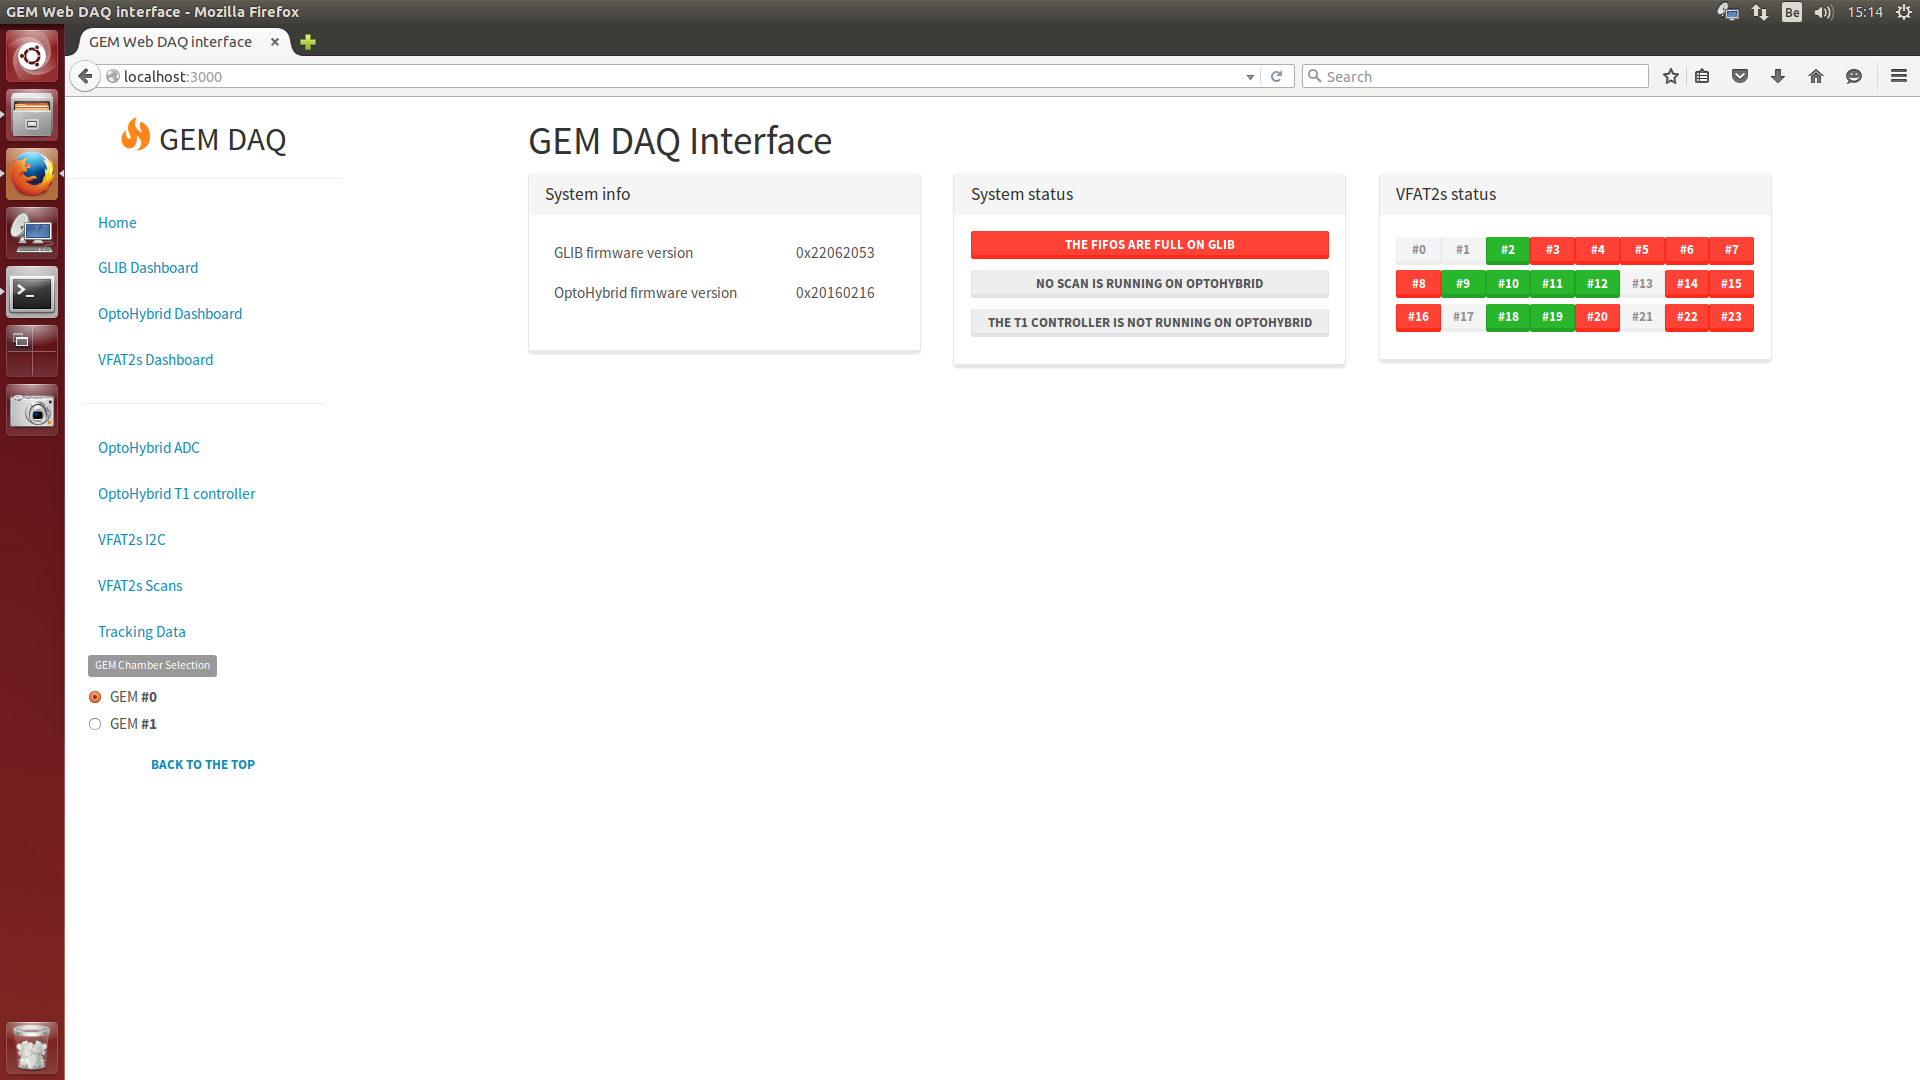
\includegraphics[width=\textwidth]{img/II-3-test-beam/app-home.png}
        \caption{Screenshots of the home page of the web application used to control and monitor the components of the DAQ system.}
        \label{fig:II-3-app-home}
      \end{figure}

      The control page of the GLIB is shown in Figure \ref{fig:II-3-app-glib}. The information it contains is mainly related to counters which allow to see, for example, the number of requests sent to the OptoHybrid and the number of responds received. It also counts the number of errors detected on the optical link providing a quantitative value of the health of the link. \\

      \begin{figure}[p!]
        \centering
        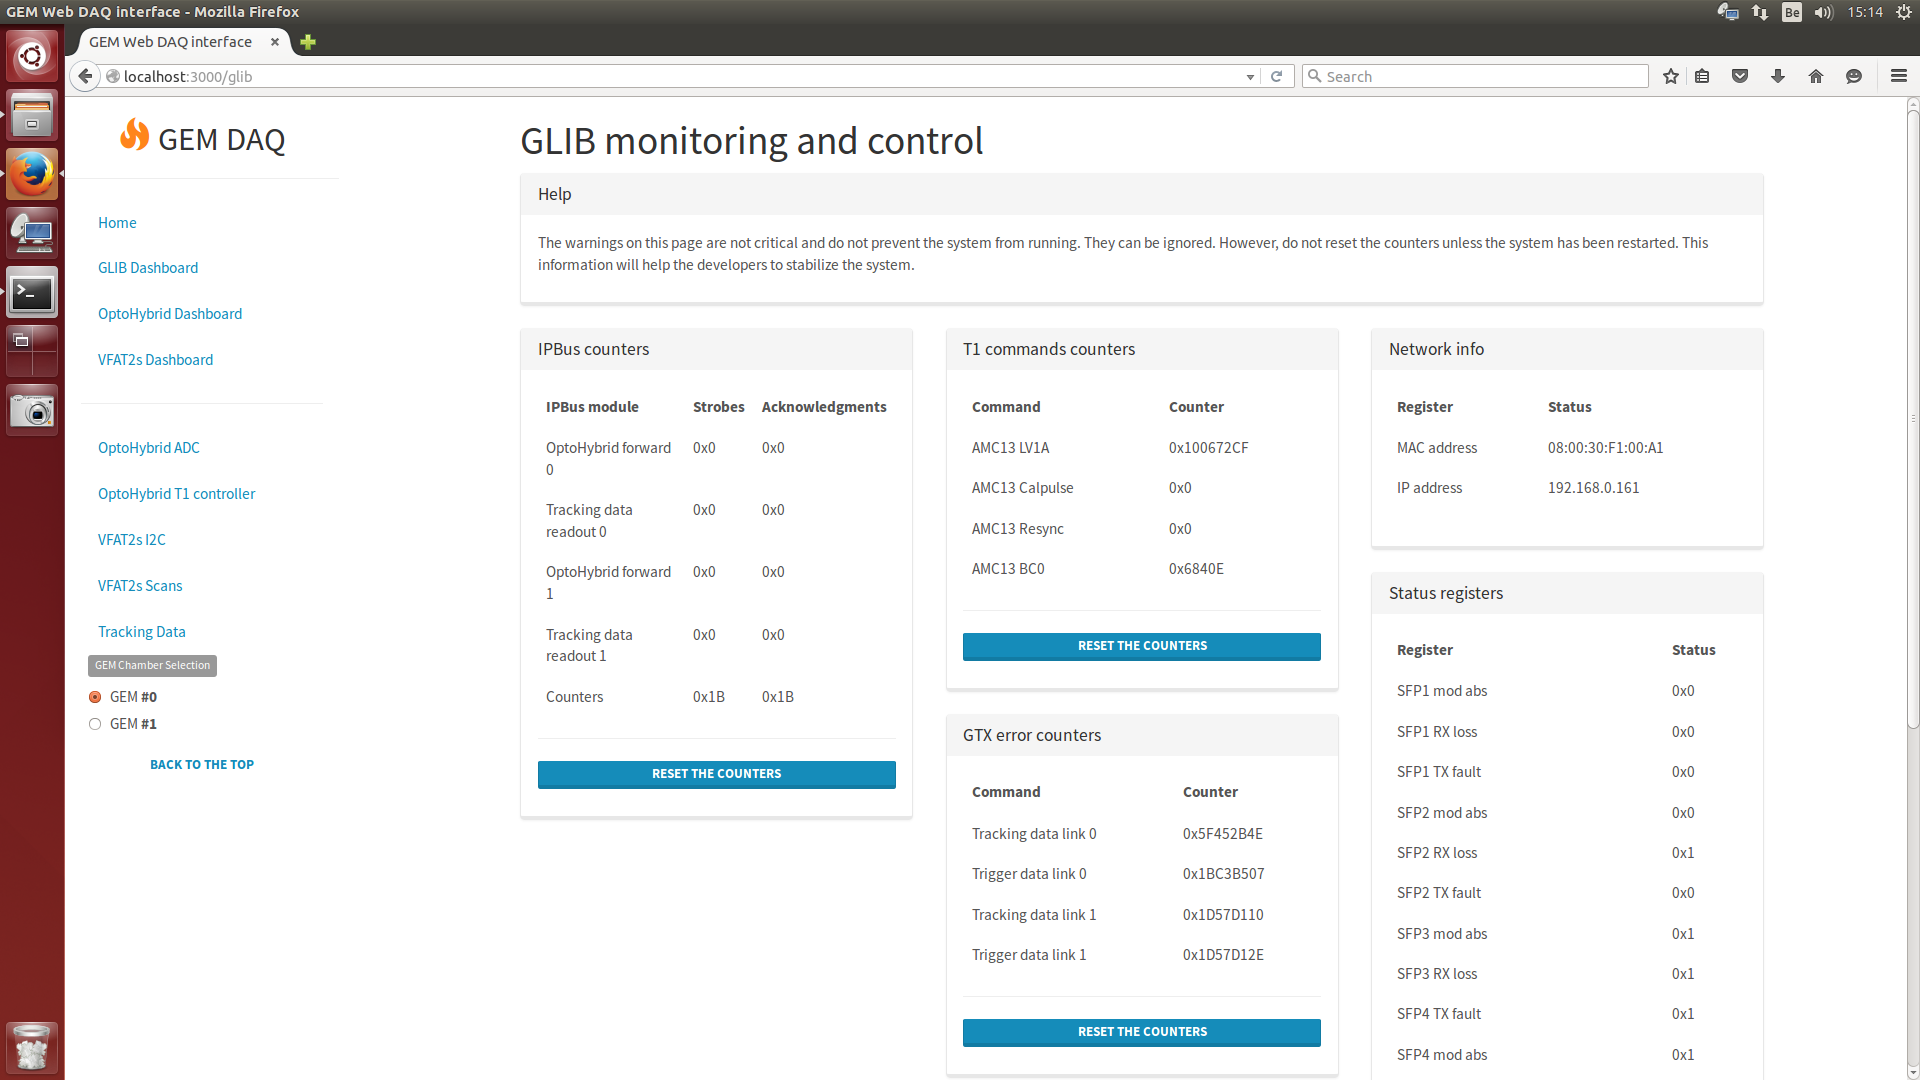
\includegraphics[width=\textwidth]{img/II-3-test-beam/app-glib.png}
        \caption{Screenshots of the page used to control and monitor the GLIB.}
        \label{fig:II-3-app-glib}
        \vspace{1cm}
        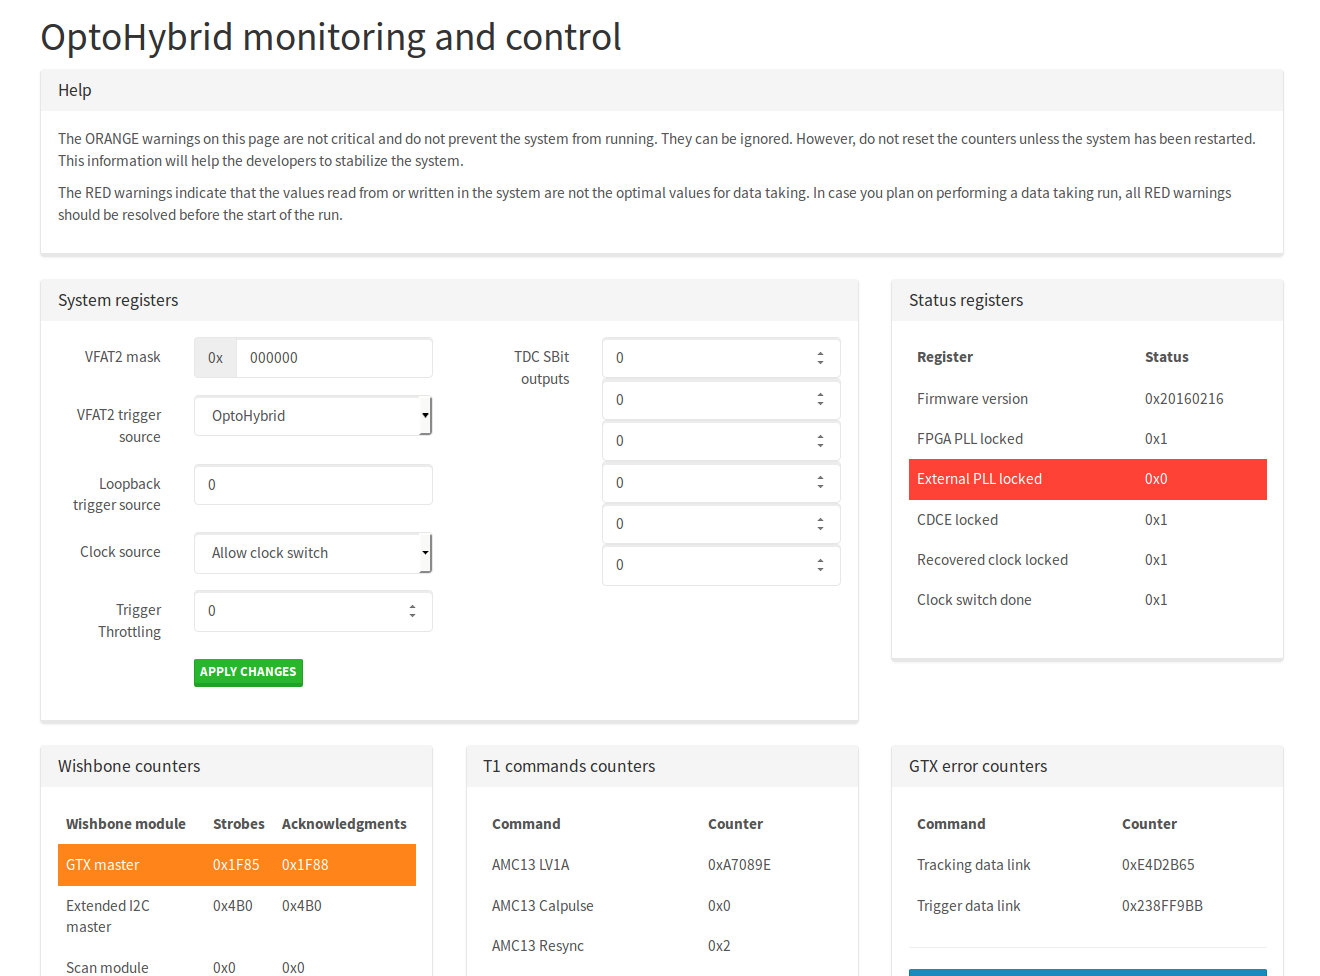
\includegraphics[width=\textwidth]{img/II-3-test-beam/app-oh.png}
        \caption{Screenshots of the page used to control and monitor the OptoHybrid.}
        \label{fig:II-3-app-oh}
      \end{figure}
      \begin{figure}[p!]
        \centering
        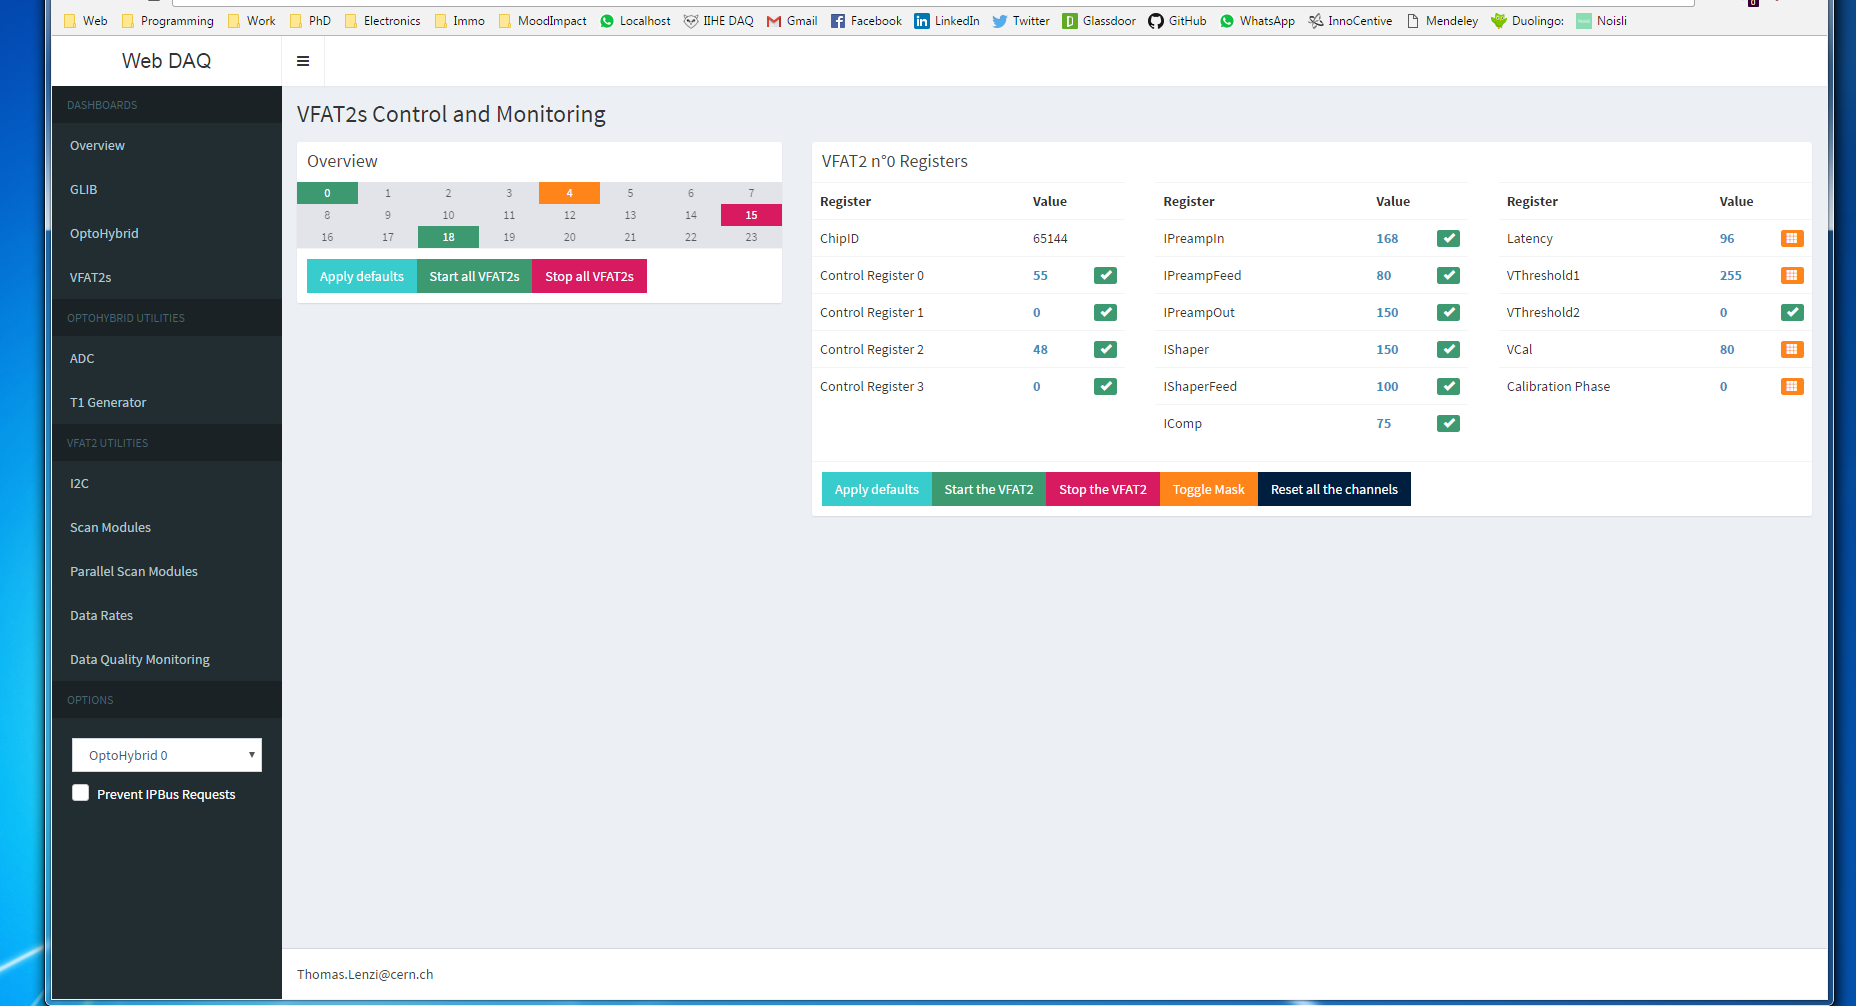
\includegraphics[width=\textwidth]{img/II-3-test-beam/app-vfat2.png}
        \caption{Screenshots of the page used to control and monitor the VFAT2.}
        \label{fig:II-3-app-vfat2}
        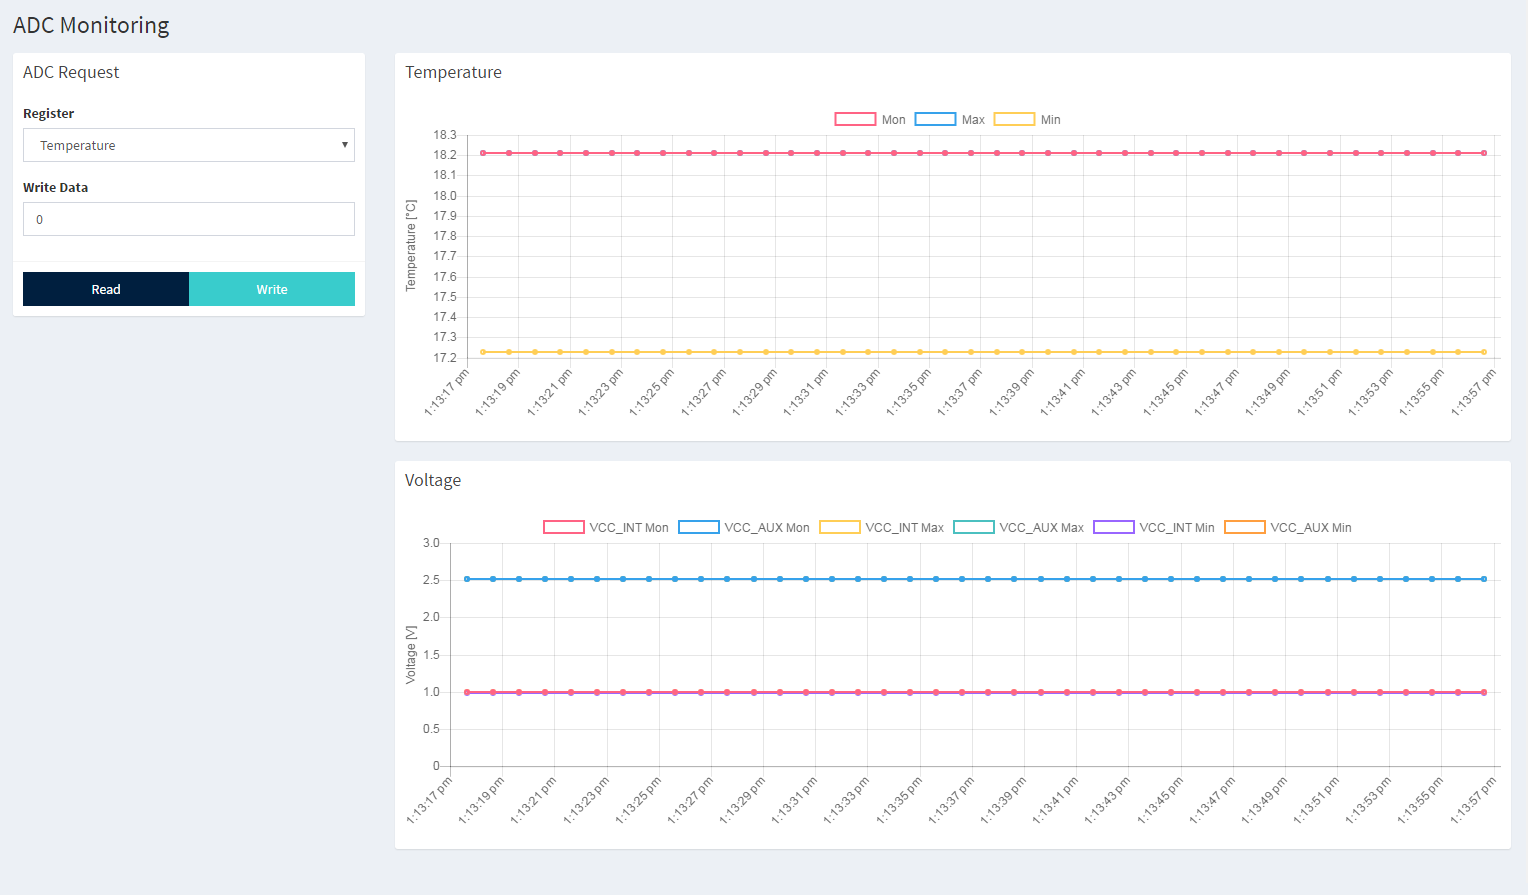
\includegraphics[width=\textwidth]{img/II-3-test-beam/app-adc.png}
        \caption{Screenshots of the page used to control and monitor the VFAT2.}
        \label{fig:II-3-app-adc}
      \end{figure}

      The OptoHybrid page, shown in Figure \ref{fig:II-3-app-oh}, provides more information and control options to the user. The top-left part of the page is used to modify system register controlling the trigger source, clock source, trigger information sent over the debugging header, etc. This is where the user can change the type of ongoing run by going from a data taking run using external triggers to a calibration run using internally generated triggers. The panel directly on the right provides status information on the various clocking resources in the FPGA. By default, the OptoHybrid uses the on-board oscillator to power the system and the optical links. As communication is established with the GLIB, the GTXs provide the recovered clock from the link which is the system clock. When the latter is stable, the OptoHybrid can decide to switch from its on-board clock to the system clock in order to be synchronous with the whole DAQ system. This operation can be prohibited, forced, or allowed by the user, which can also chose to use an external clock provided through the debugging header. These clocking options are useful for the test beam setup where the clock can be provided externally to synchronize with other electronics equipment. Finally, the bottom part of the page display counter values for the wishbone request, fast commands, link errors, etc. Note that when a discrepancy is observed between two correlated counters, a warning flag is raised as can be seen in the bottom-left of the picture. \\

      Finally, the control page of the VFAT2s, shown in Figure \ref{fig:II-3-app-vfat2}, gives access to the most significant registers of the front-end chips. It provides a summary of the on/off/absent status of each VFAT2 on the GEB and, by clicking on an individual slot, the value of each register as shown in the panel on the right. Default settings for the registers are saved in memory and compared to the current values, raising warnings when they differ and allowing the user to correct them. The user can also control all the VFAT2s at once by applying the default settings or turning them on or off at the same time. In the bottom panel, control buttons allow to mask individual VFAT2s in case they generate noise or send corrupted tracking data. Two counters monitor the number of valid (with a correct CRC) and invalid packets each position has sent.



    \subsection{Fast and Slow Control of the VFAT2s}

      The fast control or T1 generator is controlled by a dedicated page, displayed on the top of Figure \ref{fig:II-3-app-control}, which allows to select the type of commands to generate, the pattern to send, and the delay between two pulses. The slow control of the VFAT2s handled by the I2C modules and the extended I2C controller is managed by another page shown on the bottom. The slow control commands can either target a single VFAT2 as shown in the left panel or an entire set of chips as can be seen in the right panel. In case of a single command, the response is shown inline. For multiple operations, a table of results is shown indicating the value and the corresponding VFAT2. To help the user, the accessible registers are named rather than listed using their address.

      \begin{figure}[p!]
        \centering
        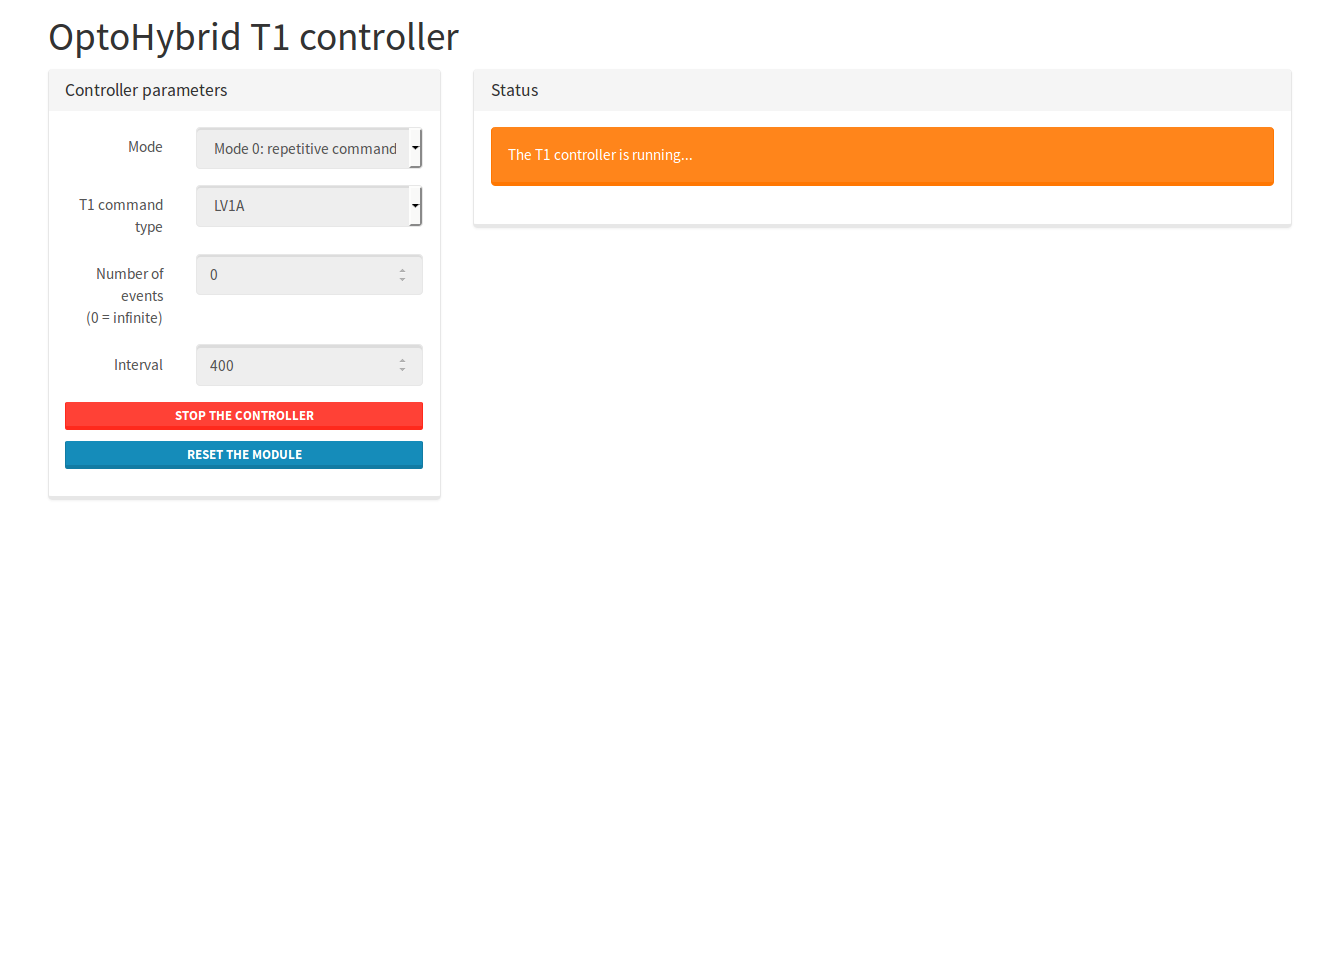
\includegraphics[width=\textwidth]{img/II-3-test-beam/app-t1.png}
        \vspace{0.5cm}
        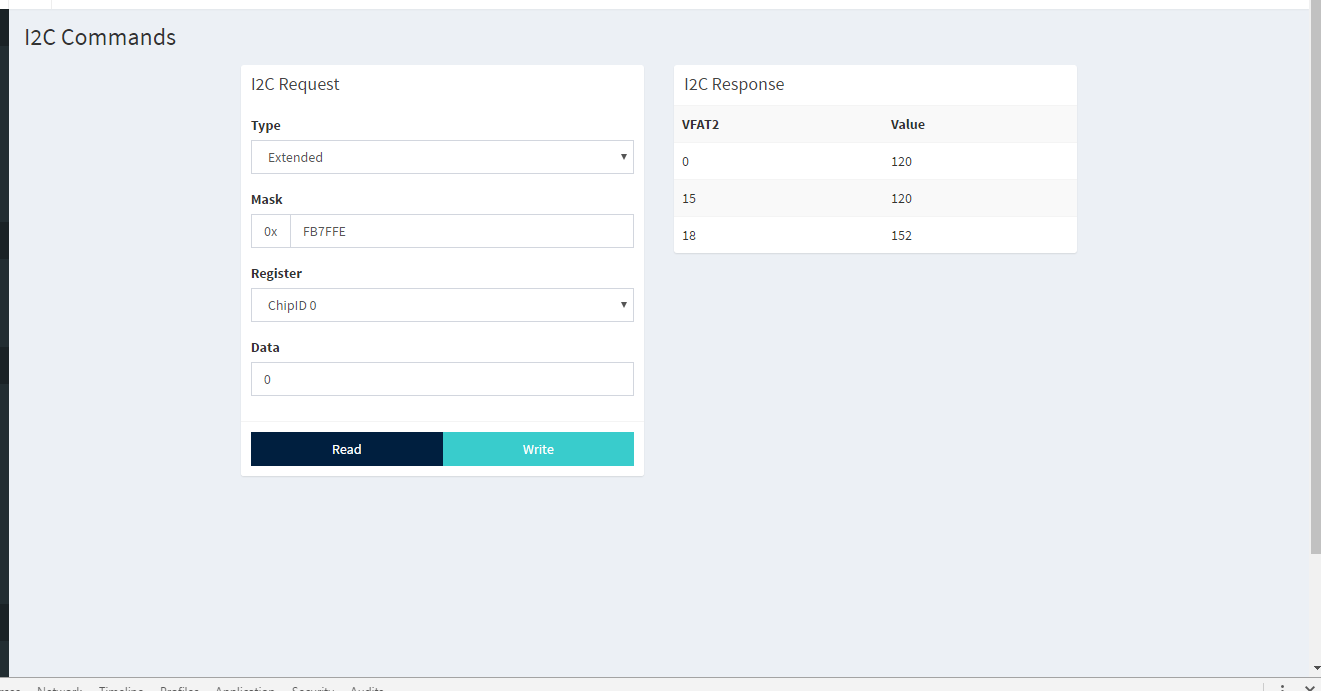
\includegraphics[width=\textwidth]{img/II-3-test-beam/app-i2c.png}
        \caption{Screenshots of the pages of the web application used to send fast commands (top) and slow control (bottom) requests to the VFAT2s.}
        \label{fig:II-3-app-control}
        \vspace{1cm}
        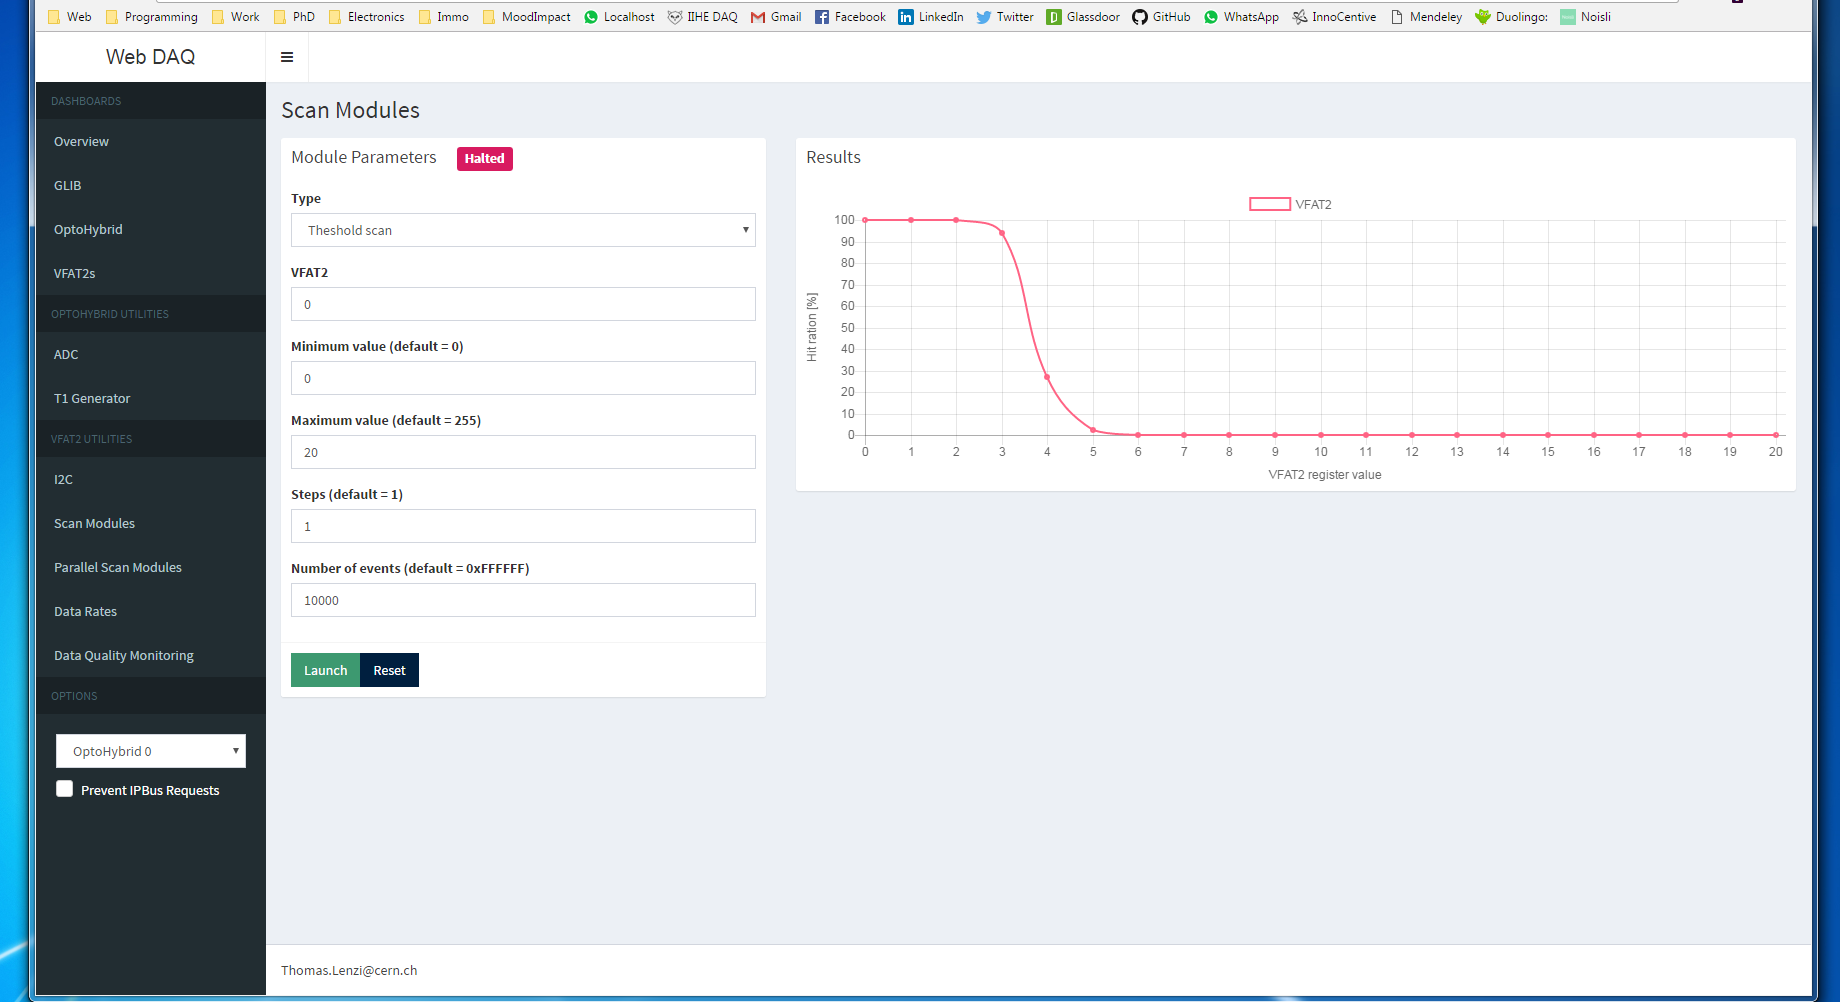
\includegraphics[width=\textwidth]{img/II-3-test-beam/app-scan.png}
        \caption{Screenshot of the page of the web application used to perform calibration scans of the VFAT2s.}
        \label{fig:II-3-app-calibration}
      \end{figure}

    \subsection{Calibrating the VFAT2s}

      The calibration of the VFAT2s is done through a dedicated page which regroups the various operations that can be performed on the chip. Figure \ref{fig:II-3-app-calibration} is a screenshot of the application running a threshold scan on one of the VFAT2s. The left panel allows the user to select all the required parameters such as the type of scan, the range of the scan, the number of events per point, etc. Once the parameters are entered, the user starts the scan and waits for it to finish in firmware. When done, a graph displays the results in the right panel. The user can then dynamically change VFAT2 settings by clicking on a point of the graph to, for example, select the most appropriate threshold or latency value. Furthermore, the user can save the data points to disk for offline analysis.

    \subsection{Data Quality Monitoring}

      DQM is used online to check the consistency of the recorded data. This is the last component of the application shown in Figure \ref{fig:II-3-app-tk}. This page monitors the status of the readout buffers of the GLIB and allows the user to acquire data. Once acquisition has started, plots begin to fill with the various parameters extracted from the VFAT2 data format. The user can visualize the number of data packets, BC, EC, flags, and chip ID distribution, the occupancy of the channels, etc, effectively monitoring the validity of the data and if required change the parameters of the run. Although this application has the ability to readout data and store it to disk, this feature was not used to this intend during the test beam. A program developed by the software development team of the GEM collaboration was used to acquire raw data from the GLIB and store it on disk in text files for later analysis.

      \begin{figure}[t!]
        \centering
        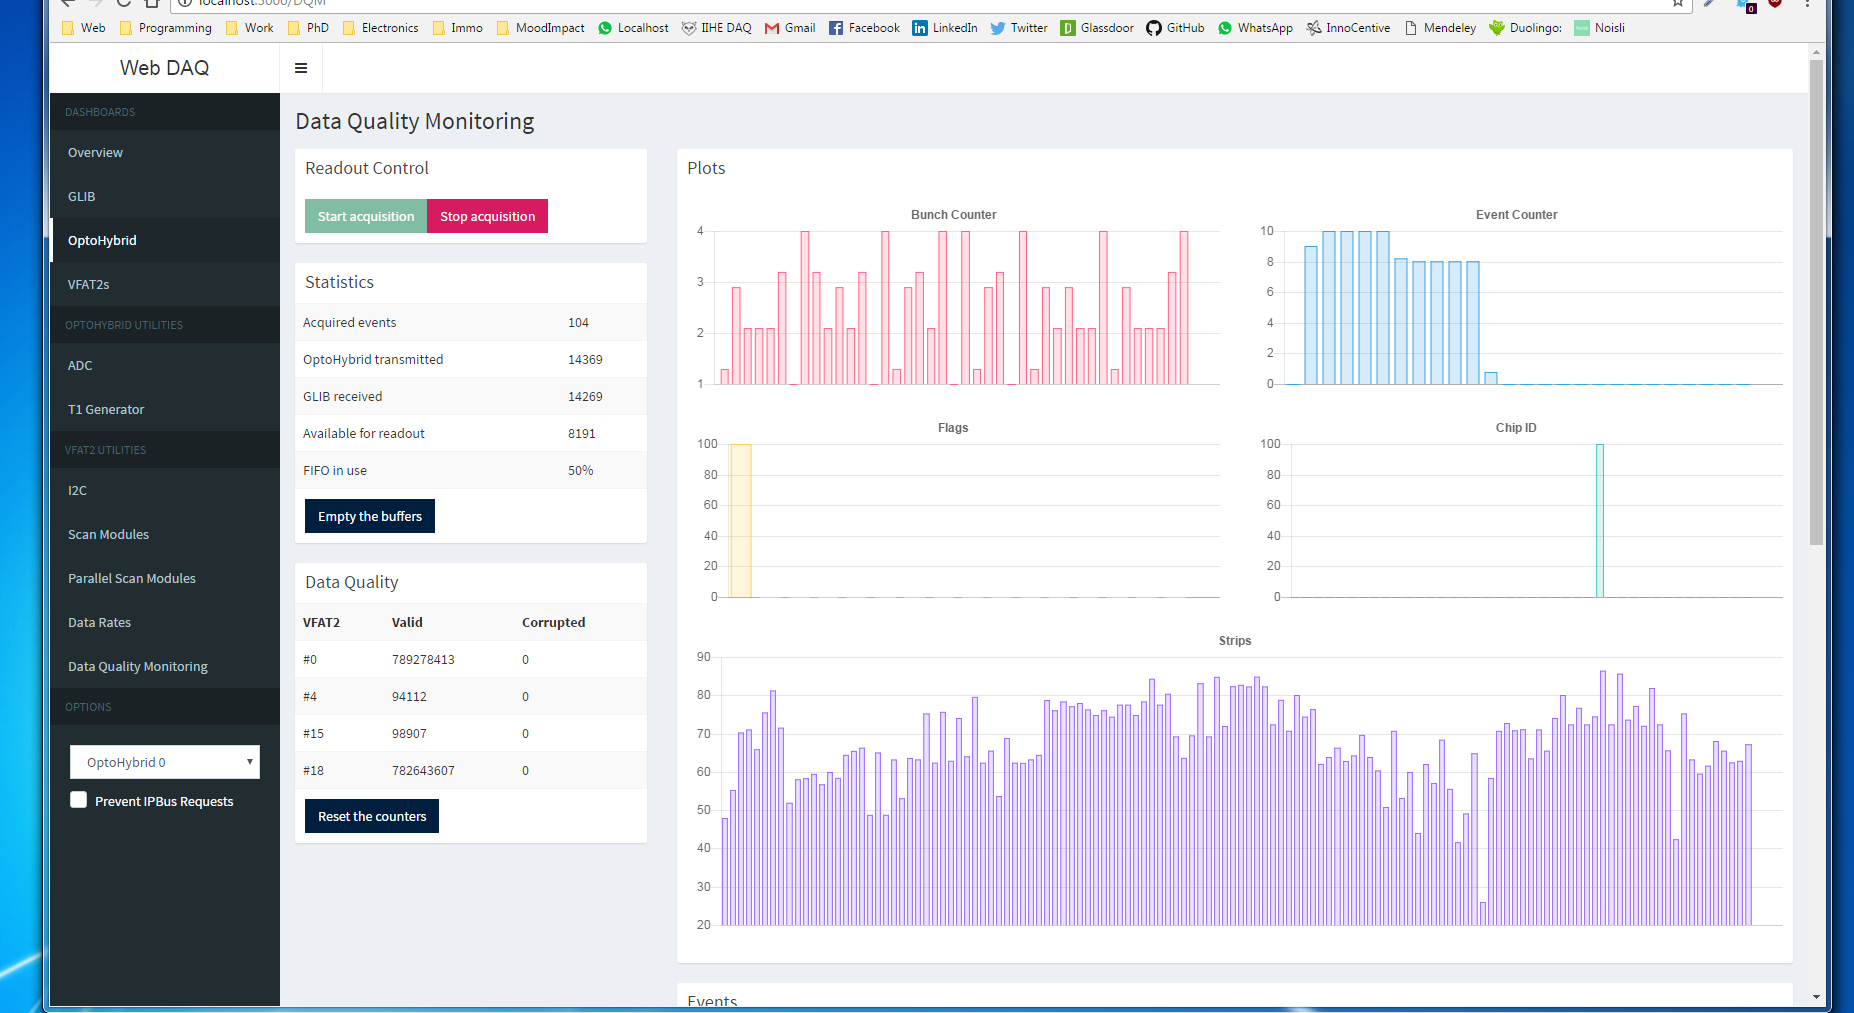
\includegraphics[width=\textwidth]{img/II-3-test-beam/app-dqm.png}
        \caption{Screenshot of the page of the web application used to do online data quality monitoring.}
        \label{fig:II-3-app-tk}
      \end{figure}

  \section{The Test Beam Setup}

    The test beam campaigns took place at CERN in the North Area of Prevessin, one of the secondary sites. The beam provided to the experiments originates from the SPS proton bunches which are extracted from the accelerator at 400 GeV and interact with a 30-cm-thick Beryllium target to produce the secondary beams mainly composed of electrons and hadrons (protons, pions, and kaons). A selection on the type of particles and their momentum is performed using so-called wobbling magnets that bend the beams and redirect them to the experimental setups. In the transfer tunnels, collimators can be adjusted to increase or reduce the flux of particles and an optional secondary target can be placed in the beam path to create a tertiary beam. Figure \ref{fig:II-3-sps} shows the monitoring page of the SPS indicating the presence of spills of particles in yellow. Spills last between 4.8 s and 9.6 s and repeat every 14 s to 48 s depending on the SPS operation. \\

    \begin{figure}[t!]
      \centering
      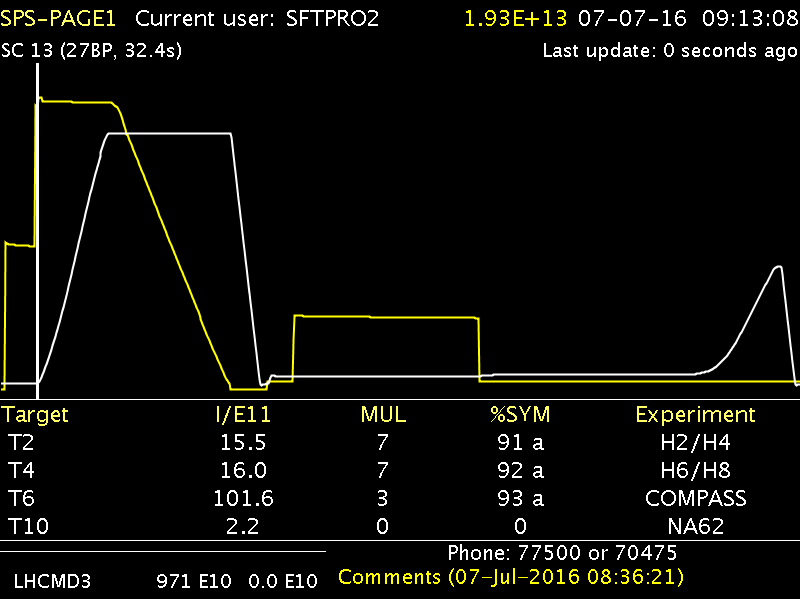
\includegraphics[width=0.8\textwidth]{img/II-3-test-beam/sps.png}
      \caption{Monitoring page of the SPS indicating the presence of spills of particles (yellow).}
      \label{fig:II-3-sps}
    \end{figure}

    The two types of particles used during the test beam were 150 GeV pions and muons. Pions are obtained from the secondary beam by inserting a thin absorber which removes the electronic component of the beam. They can reach intensities between 10$^4$ and 10$^7$ particles per spill and produce a very narrow beam of around 5 cm in diameter. From their decay, a muon beam can be obtained by using moderate intensity secondary beams and closing the collimators. The muon beam reaching the experimental setup is a wider, with a diameter around 14 cm, and with an intensity of 1\% of the incident proton beam.

    \subsection{The GEM Detectors Setup}

      During the November 2015 test beam campaign, two GE1/1-V detectors have been used to collect data. The first detector in the beam will be referred to as GEM0 and the second as GEM1. Each detector was equipped with 12 VFAT2 Hybrids mounted in the central four rows. The remaining slots, too far away from the beam spot, were covered with grounding equipment to reduce noise. Each GEM was mounted with a GEB v2 and a OptoHybrid v2a. A picture of the setup is shown in Figure \ref{fig:II-3-test-geb}. Both OptoHybrids were connected to the same GLIB placed in a microTCA crate. \\

      \begin{figure}[p!]
        \centering
        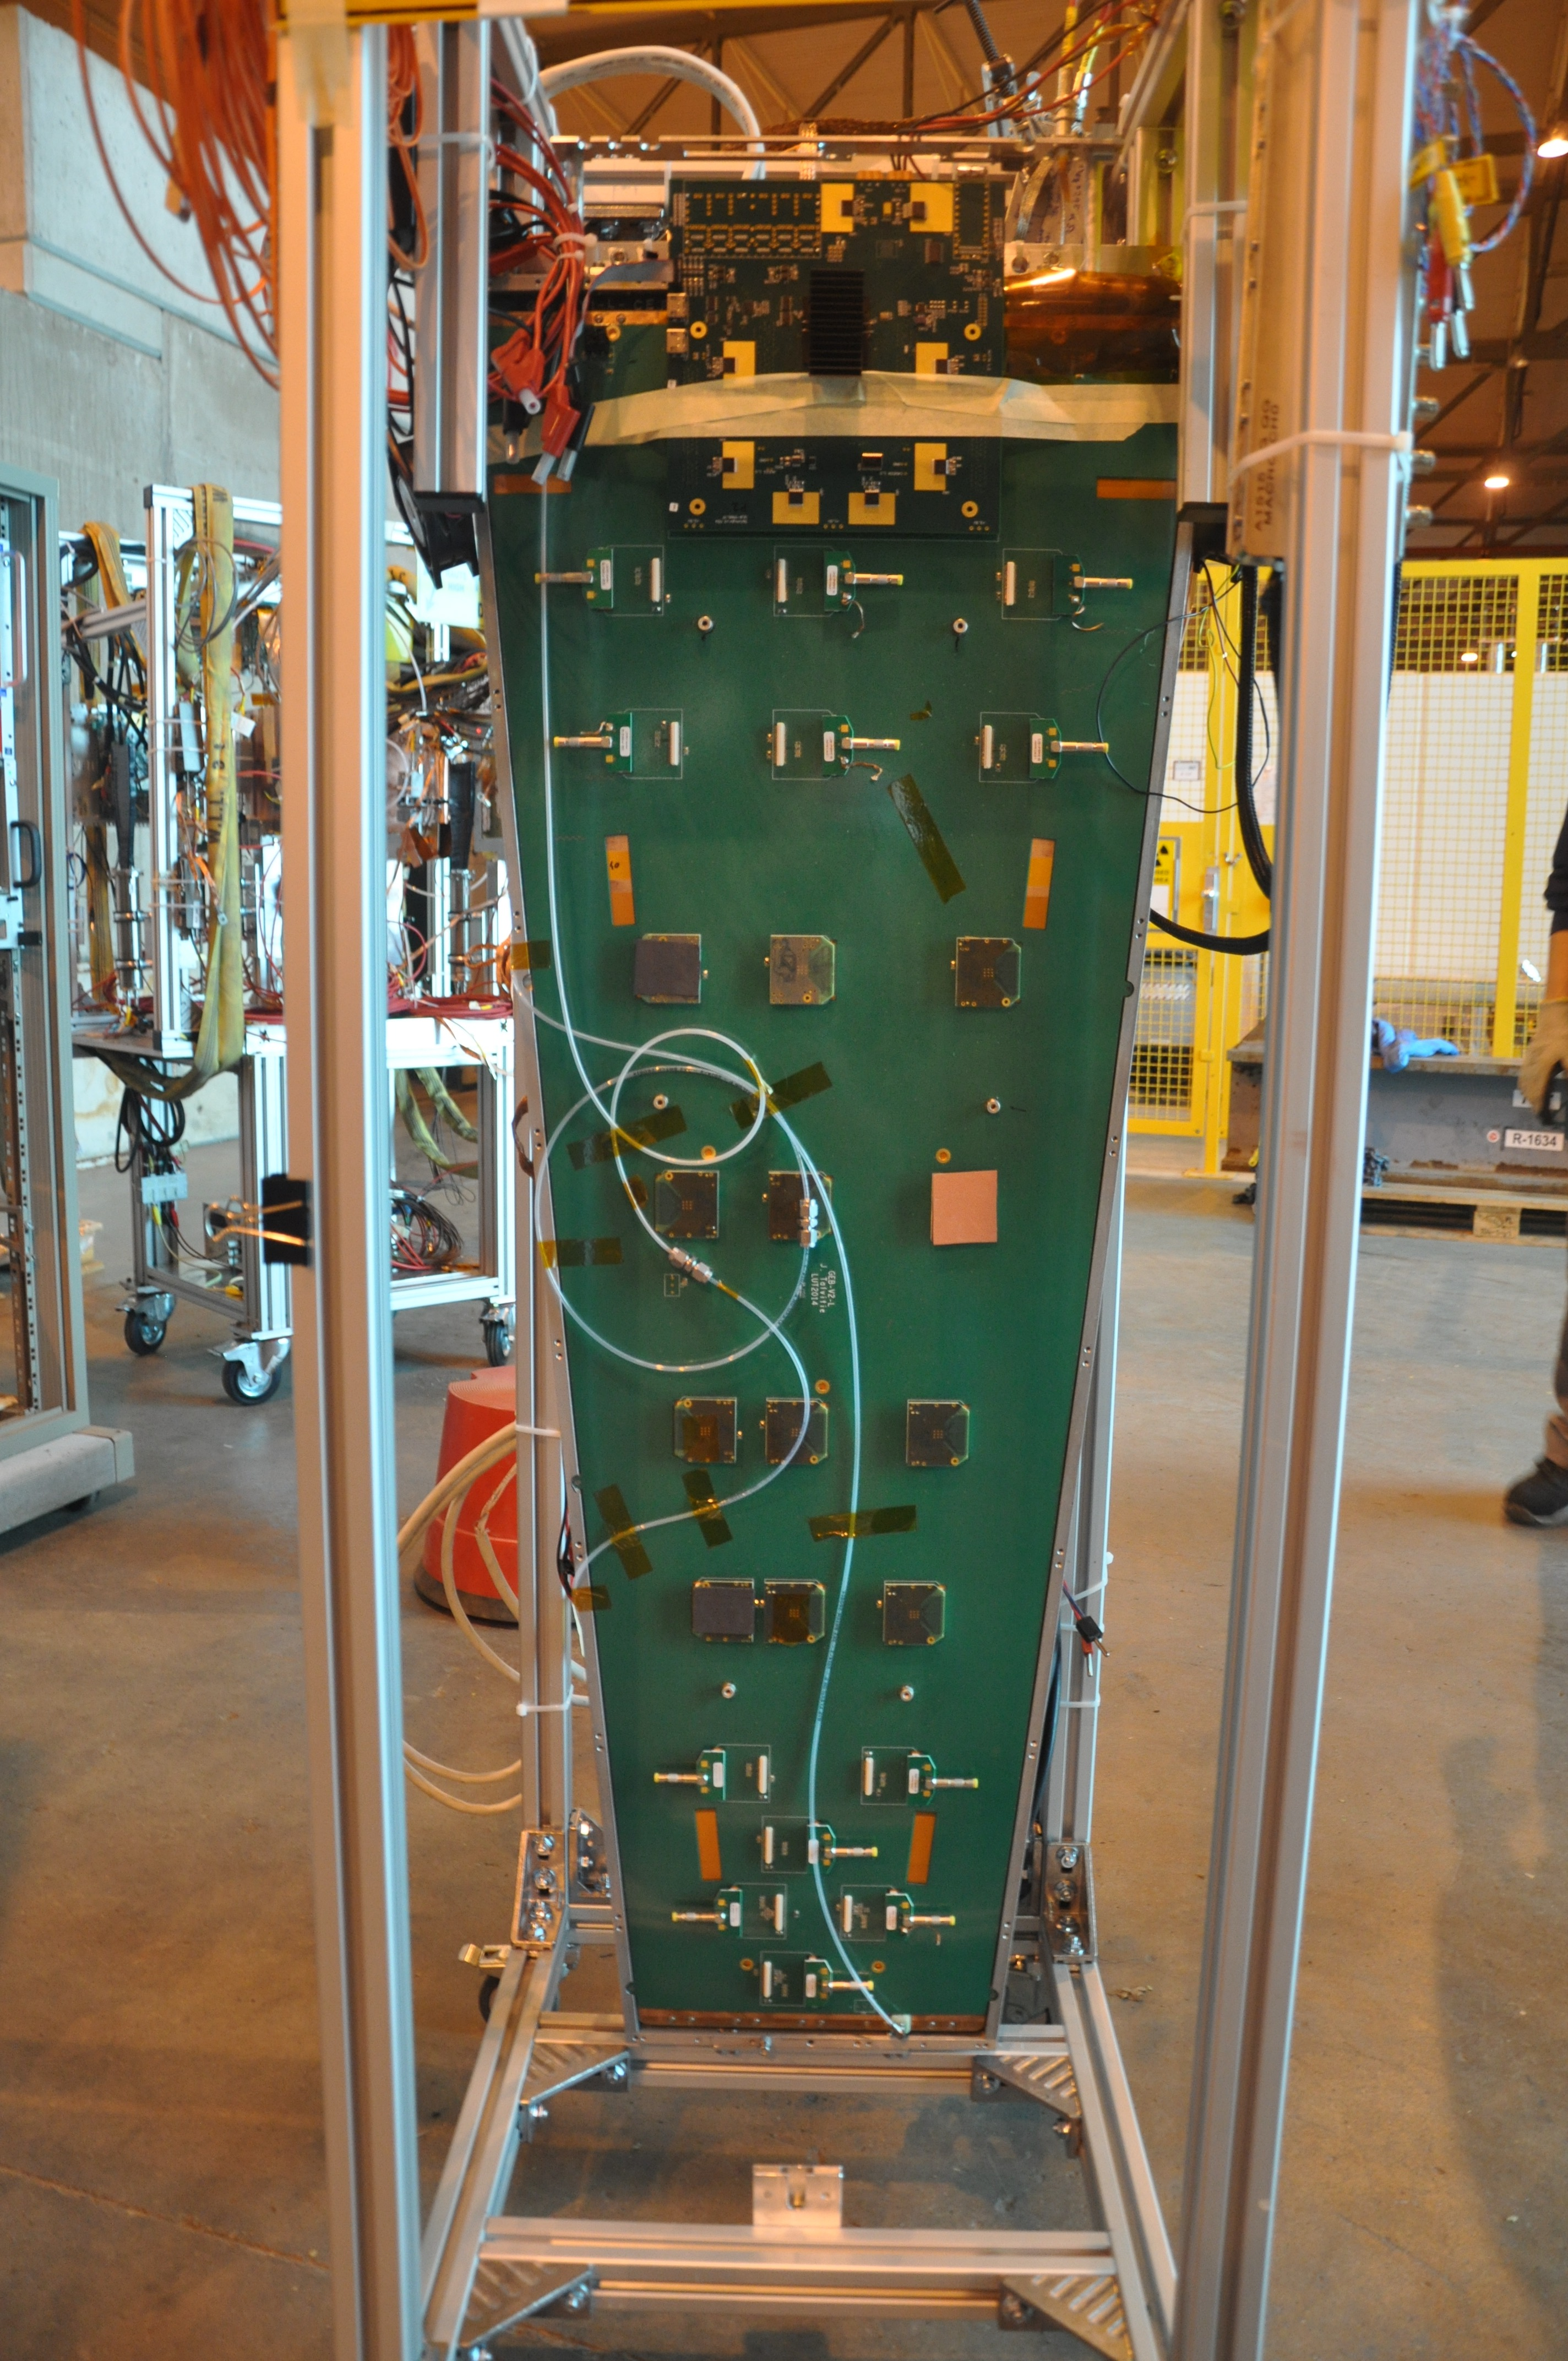
\includegraphics[width=\textwidth]{img/II-3-test-beam/test-geb.jpg}
        \caption{Photograph of the GEM detectors used during the test beam and equipped with the full electronics system.}
        \label{fig:II-3-test-geb}
      \end{figure}

      The GEM detectors were connected to a gas system providing a mixture of Ar/CO$_2$/CF$_4$ at 45\%, 15\%, and 40\% respectively. The high-voltage was delivered through a ceramic high-voltage divider for one chamber and by separate channels connected directly to the GEM foils and planes for the other. The high-voltage applied is expressed in terms of current flowing through the divider which, by summing up the individual resistors that it is made of, yields a value in volts. Table \ref{tab:II-3-test-hv} enumerates the different values of the voltages according to the current flowing through the divider. The difference between the divider and drift plane values is due to an input filter placed before the latter which smooths out fluctuations in the voltage. The low voltages for the OptoHybrids (1.8 V and 4 V) and for the GEBs (2.5 V) were delivered by two power boards mounted on top of the detector stand, along with the necessary tools to reprogram the FPGA in case of failure and the debugging headers. \\

      \begin{table}[h!]
        { \footnotesize
        \begin{tabularx}{\textwidth}{|C{1}|C{1}|C{1}|C{1}|C{1}|C{1}|C{1}|C{1}|C{1}|}
          \hline \textbf{Current ($\mu$A)} & \textbf{Divider (V)} & \textbf{Drift plane (V)} & \textbf{GEM1 top (V)} & \textbf{GEM1 bottom (V)} & \textbf{GEM2 top (V)} & \textbf{GEM2 bottom (V)} & \textbf{GEM3 top (V)} & \textbf{GEM3 bottom (V)} \\ \hline
          700 & 3921 & 3290 & 2503 & 2107 & 1801 & 1416 & 805 & 437 \\
          710 & 3977 & 3337 & 2538 & 2137 & 1827 & 1437 & 816 & 443 \\
          720 & 4033 & 3384 & 2574 & 2167 & 1853 & 1457 & 828 & 450 \\
          730 & 4089 & 3431 & 2610 & 2198 & 1879 & 1477 & 839 & 456 \\
          740 & 4145 & 3478 & 2646 & 2228 & 1904 & 1497 & 851 & 462 \\
          750 & 4201 & 3525 & 2682 & 2258 & 1930 & 1518 & 862 & 468  \\
          760 & 4257 & 3572 & 2717 & 2288 & 1956 & 1538 & 874 & 475 \\
          770 & 4313 & 3619 & 2753 & 2318 & 1981 & 1558 & 885 & 481 \\
          780 & 4369 & 3666 & 2789 & 2348 & 2007 & 1578 & 897 & 487 \\
          790 & 4425 & 3713 & 2825 & 2378 & 2033 & 1598 & 908 & 493 \\
          800 & 4481 & 3760 & 2860 & 2408 & 2059 & 1619 & 820 & 500 \\
          810 & 4537 & 3807 & 2896 & 2438 & 2084 & 1639 & 931 & 506 \\ \hline
        \end{tabularx}
        }
        \caption{Values of the voltages applied to the detectors according to the current flowing through the high voltage resistive divider.}
        \label{tab:II-3-test-hv}
      \end{table}

      The high voltage applied on the drift plane can be converted to an effective gas gain for the Triple-GEM detector. Figure \ref{fig:II-3-gain} shows the measured gas gains as a function of the current through the high voltage divider for the different generations of GEM detectors and for ArCO$_2$ 70:30 and ArCO$_2$CF$_4$ 45:15:40.

      \begin{figure}[t!]
        \centering
        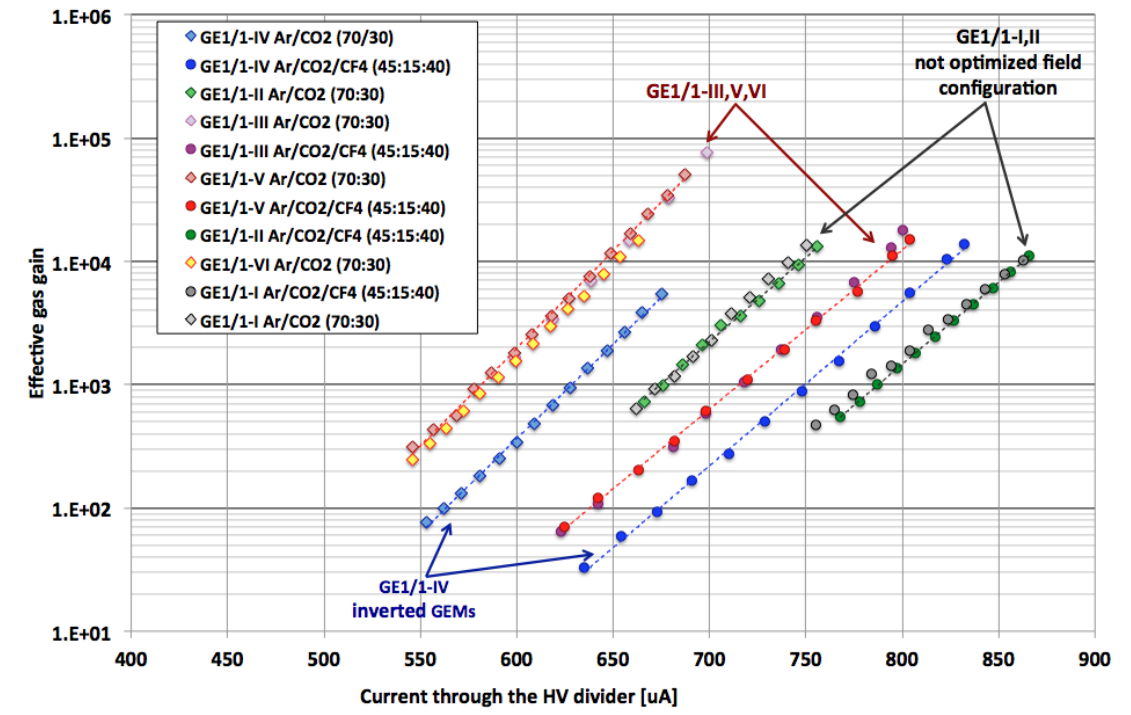
\includegraphics[width=0.9\textwidth]{img/II-3-test-beam/gain.png}
        \caption{Measured gas gains as a function of the current through the high voltage divider for the different generations of GEM detectors and for ArCO$_2$ 70:30 and ArCO$_2$CF$_4$ 45:15:40 \cite{Merlin:2155685}.}
        \label{fig:II-3-gain}
      \end{figure}

    \subsection{The Beam Area Setup}

      The GE1/1 detectors were inserted in the beam path and adjusted so that only one VFAT2 in the middle column would be exposed to the beam spot. Figure \ref{fig:II-3-test-setup} shows the setup on the left placed in front of the beam transfer tunnel on the right side. Four scintillators, three placed in front of the detector and visible in the picture, and one placed in the back of the detector were used to provide triggers to the system. The output of the four scintillators was converted to Nuclear Instrumentation Module (NIM) logic and their coincidence used as the asynchronous trigger source of the system. \\

      \begin{sidewaysfigure}[p!]
        \centering
        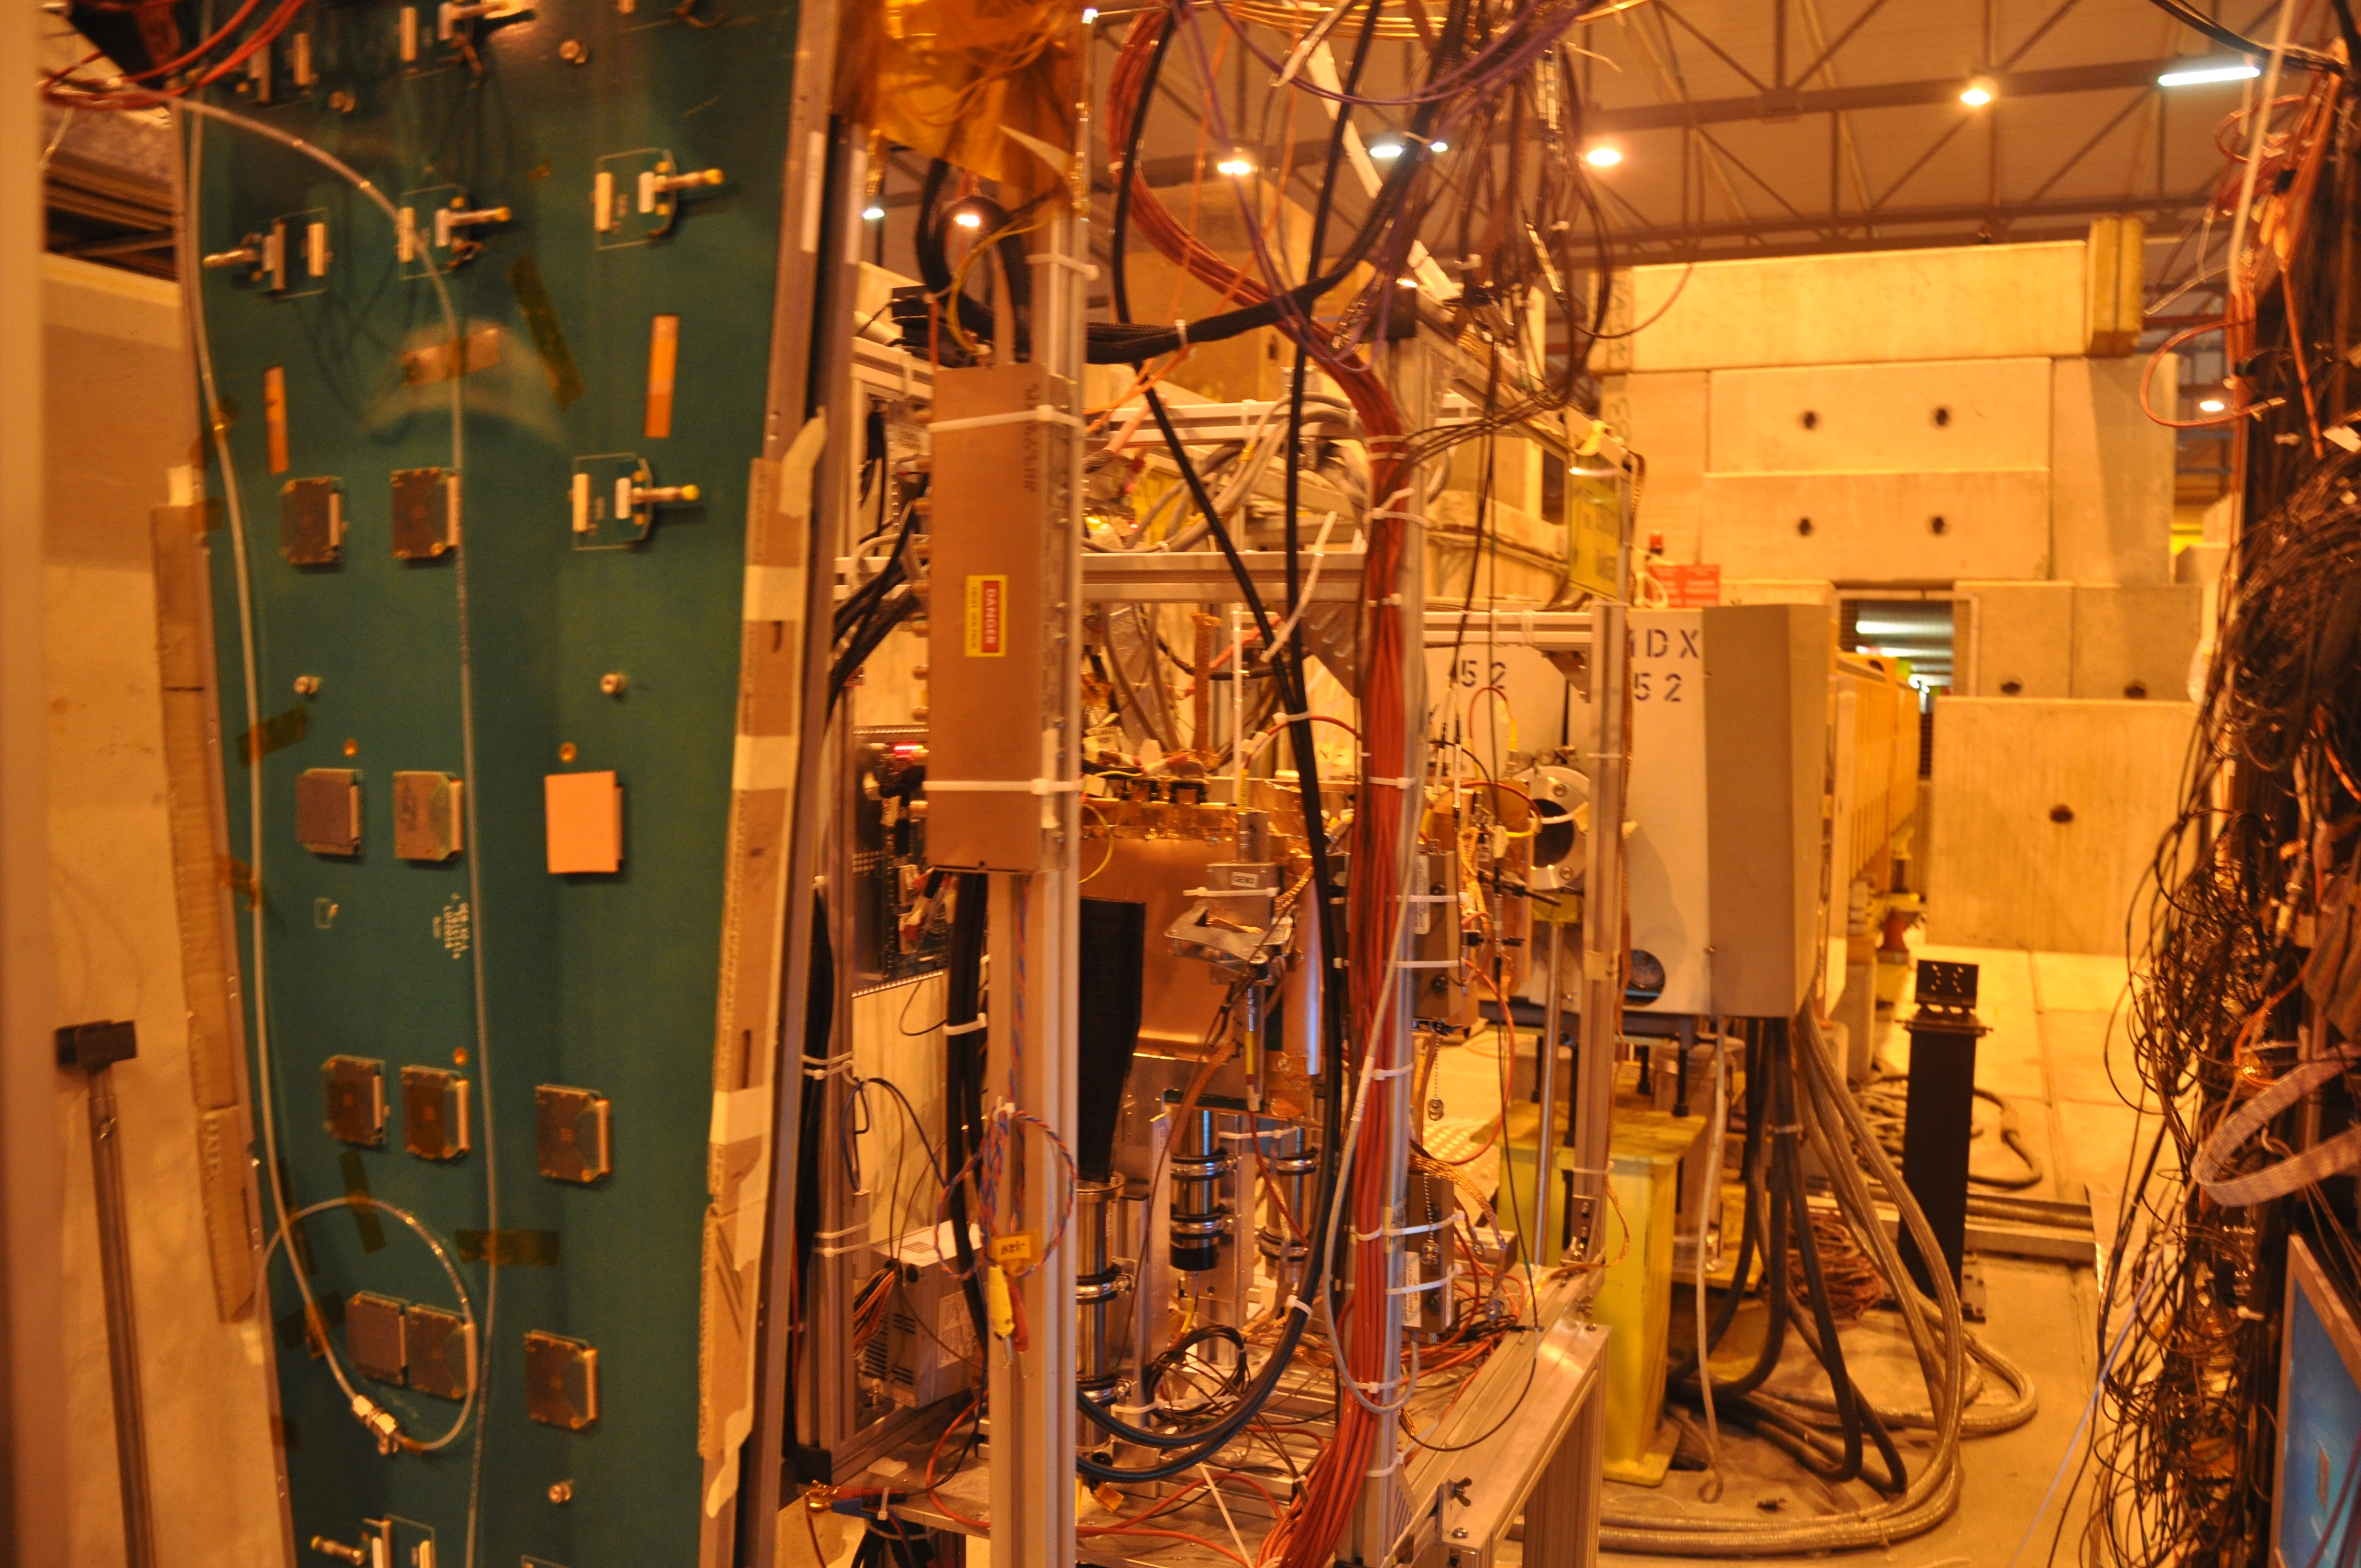
\includegraphics[width=0.9\textwidth]{img/II-3-test-beam/test-setup.jpg}
        \caption{Photograph of the two detectors on the left placed in front of the beam transfer tunnel on the right side.}
        \label{fig:II-3-test-setup}
      \end{sidewaysfigure}

      NIM uses current driven logic levels which produce -0.8 V over 50 $\Omega$ for a logic '1' and 0 V for a logic '0'. As the OptoHybrids use TTL voltage driven levels, namely 2.5 V for a logic '1' and 0 V for a logic '0', a converter had to be used. It was observed that the output levels of the NIM to TTL module were 0 V - 1.25 V instead of 0 V - 2.5 V. This is close to the switching voltage of 1.2 V and might affect the number of triggers seen by the OptoHybrids, as logic '1's might be discarded. It was computed using the offline data to count the number of missing events that this situation occurred in less than 1/10 000 events and could be solved by the offline analysis. Using other sources of triggers, it was ensured the source of the problem did not originate from the DAQ system itself, which was proven not to be the case. The problem came from the NIM to TTL converter and not the electronics of the GEM detectors.

  \section{Data Analysis}

    The data collected during the test beam was analyzed to study the performance of the detector according to various parameters. Data was taken at multiple high-voltage values, VFAT2 threshold settings, and trigger rates. An analysis framework has been developed in order to combine the readout data from the two GE1/1 chambers. Alignment of the events was non-trivial and based on the difference between two consecutive BC values of the events. Indeed, due to the problem exposed here above with the NIM to TTL converter the number of events recorded by the two detectors might not be equal. Furthermore, the fact that the two VFAT2s are not guaranteed to have the same value of the BC counter at the same time prevented the framework from using the BC directly. Therefore, the difference between the BCs of two consecutive events in the data stream was computed and matched between the two datasets. When a discrepancy arose, one of the datasets had to be realigned. Once realignment was performed, analysis tools had access to both chambers for each event. This issue will not occur in CMS as the triggers will be distributed by the AMC13 and as all the detectors will be synchronized. It will thus be possible to reset all the VFAT2s at the same time, ensuring that the BC is the same.

    \subsection{VFAT2 Threshold Scans}

      The first parameter to study is the noise on the VFAT2s induced by the system and by the effect of the channels. To this end, threshold scans have been produced using the web application. These scans are ran when the beam is not present. They use the trigger bits of the VFAT2s which do not need a L1A source to be produced. These are clocked at 40 MHz and for each threshold value the ratio of events containing hits against the total amount of collected events is defined to be the noise. Figure \ref{fig:II-3-data-threshold} plots the noise level as a function of the VFAT2 threshold in terms of VFAT2 units, the decimal value written in the eight bits register afterwards converted to a voltage level, for GEM0 on the left and GEM1 on the right with muons. Although the noise level quickly diminishes, it never reaches the expected value of 0 even at very high threshold. Typically, previous test beams have shown that a value of 15 eliminates the noise. Furthermore, it can be seen that noise level is slightly higher in GEM1, which reaches 20\% at a threshold value of 10 against 15\% for GEM0. From the threshold scans, it was decided to run both chambers at a VFAT2 threshold level of 25 for data taking runs. This value is considered to be the default threshold except if otherwise specified. \\

      \begin{figure}[b!]
        \centering
        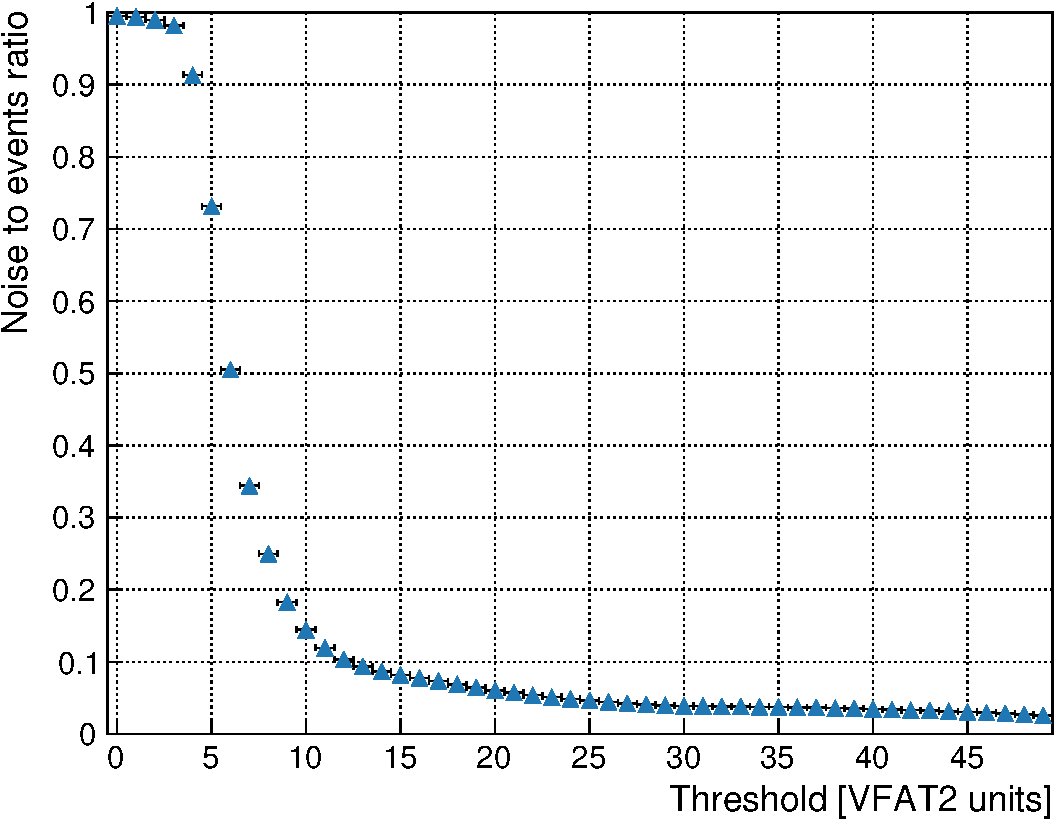
\includegraphics[width=0.49\textwidth]{img/plots/cThresholdScan_GEM0-crop}
        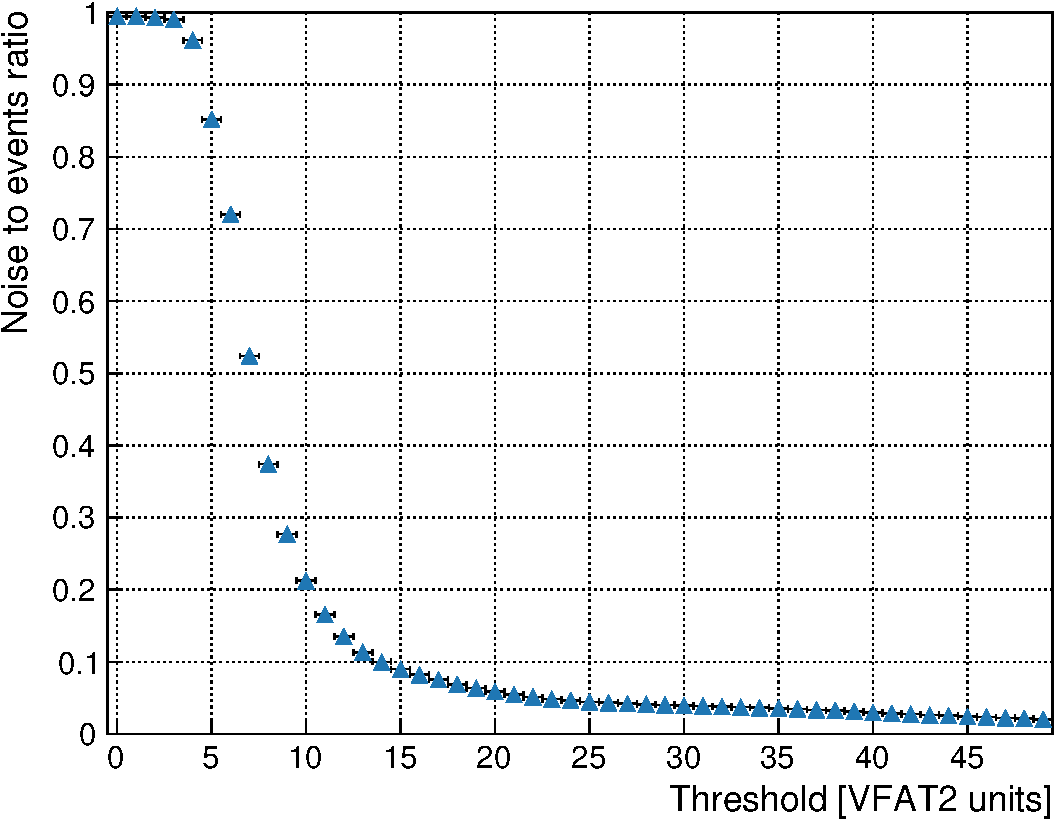
\includegraphics[width=0.49\textwidth]{img/plots/cThresholdScan_GEM1-crop}
        \caption{Plots of the noise level as a function of the VFAT2 threshold in terms of VFAT2 units, the decimal value written in the 8 bit register afterwards converted to a voltage level, for GEM0 on the left and GEM1 on the right.}
        \label{fig:II-3-data-threshold}
      \end{figure}

      After the end of the test beam, the noise issue has been investigated thoroughly and two sources have been isolated: the I2C clock used for the slow communication and the LEMO cables used for the trigger input. In the version of the firmware used during the test beam, the I2C clock ran continuously which induced noise on the trigger bits of the VFAT2s at a frequency of 100 kHz, the same as the clock itself. This problem has been solved by activating the I2C clock solely when a slow control operation takes place, limiting the number of corrupted trigger bits. The second issue originated from current loops formed between the low power cables of the OptoHybrids and the LEMO cable connecting the system to the NIM crate. The ground of the latter was connected to the OptoHybrid ground through the shielding of the LEMO cables. Once the two ground systems were isolated, noise level comparable to previous observations were obtained. Figure \ref{fig:II-3-noise-comp} plots the noise level as a function of the VFAT2 threshold in terms of VFAT2 units with results obtained during the test beam on the left and with the improved noise cancelation on the right. The reduction in noise in turn allowed to function at a lower threshold and thus increase the efficiency of the detector, reaching the required 98\% mark. \\

      \begin{figure}[t!]
        \centering
        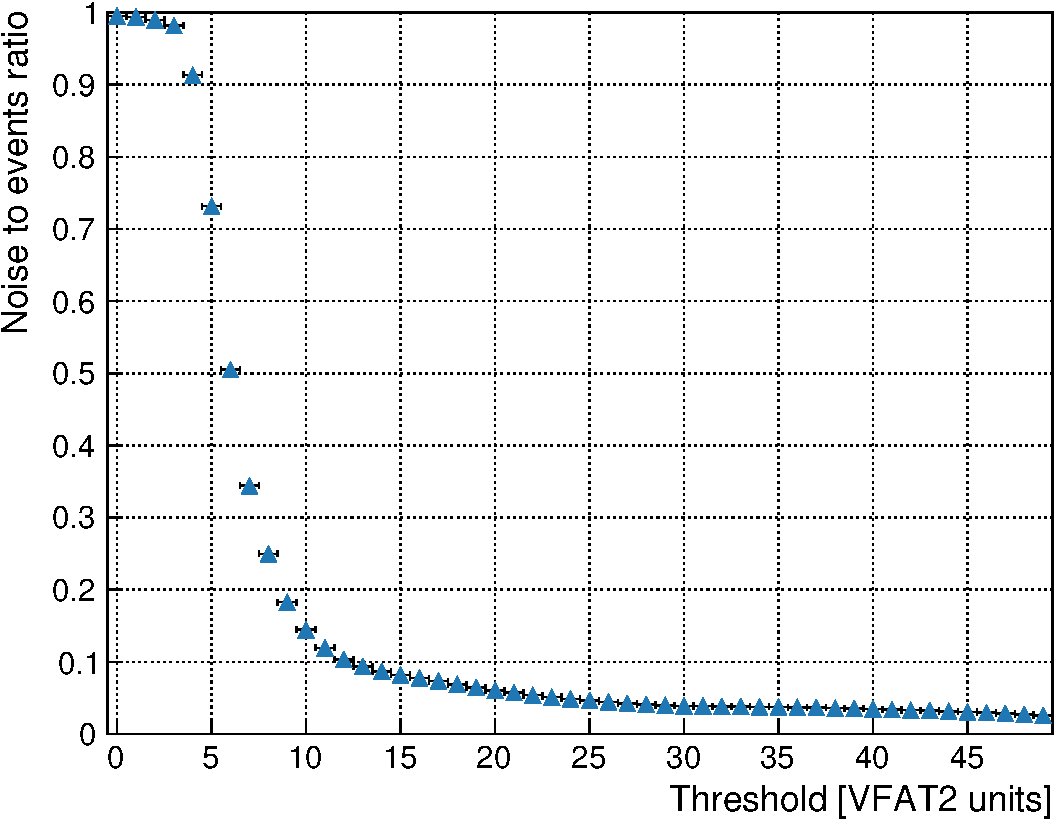
\includegraphics[width=0.49\textwidth]{img/plots/cThresholdScan_GEM0-crop}
        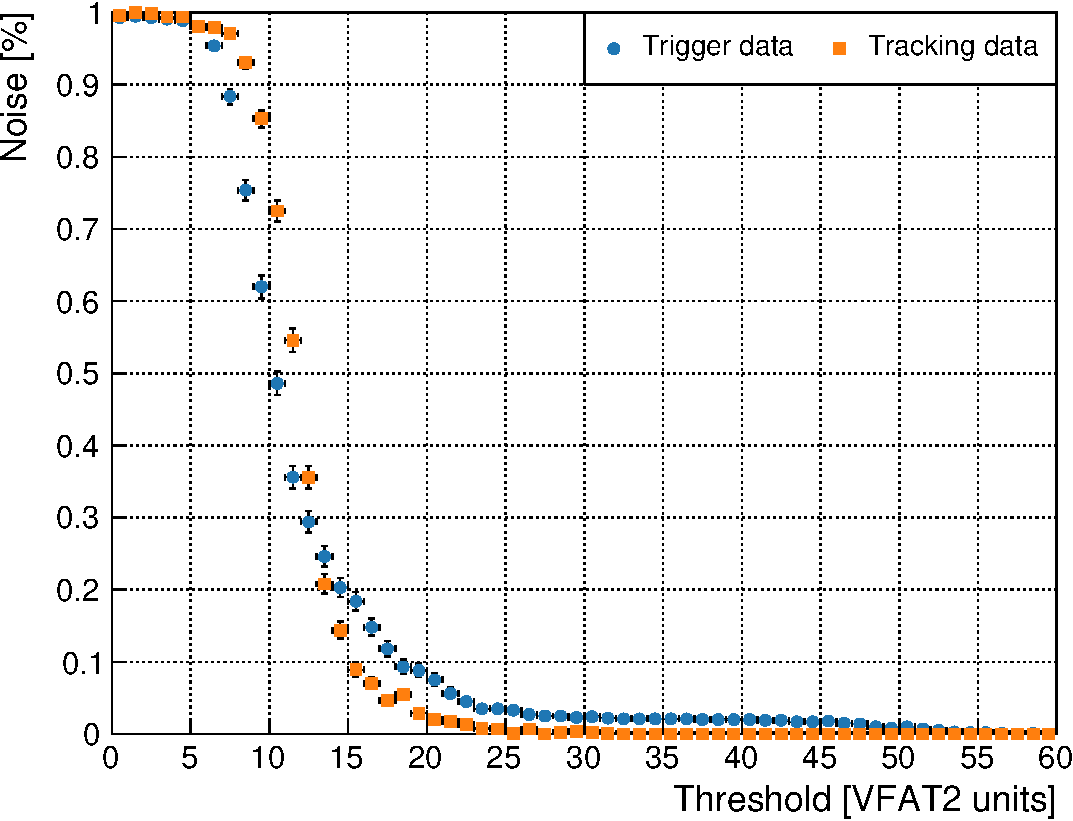
\includegraphics[width=0.49\textwidth]{img/plots/cThreshold_SBitsTK-crop}
        \caption{Plots of the noise level as a function of the VFAT2 threshold in terms of VFAT2 units with results obtained during the test beam on the left and with the improved noise cancelation on the right.}
        \label{fig:II-3-noise-comp}
      \end{figure}

      It was also observed that GEM1 experienced a leakage current through the GEM foils of about 10 $\mu$A. This had as consequence to reduce the voltage on the GEM foils and thus decrease the gain and efficiency of the detector. The detector also suffered from water condensation inside the gas pipes which caused some problems during the first days of run. These issues can explain the difference in noise observed between the two chambers.

    \subsection{VFAT2 Latency Scans}

      Once the threshold on the VFAT2s has been set and the beam turned on, a latency scan must be done in order to capture the events corresponding to the triggers coming from the scintillators. Again, the web application is used to run the scan on the VFAT2s. Similarly to the threshold scan, the latency scan counts the ratio of events with a hit against the total number of events. However, it uses the tracking data provided by the VFAT2s and not the trigger bits. Figure \ref{fig:II-3-data-latency} plots the ratio of hit events as a function of the VFAT2 latency in terms of BXs for a monostable pulse length of four clock cycles for GEM0 on the left and GEM1 on the right with muons. When the latency is too low or too high, the VFAT2 misses the hit and a baseline value of 0.05 is observed corresponding to noise. Once the latency enters the correct window, it rises to a value close to 0.98. These plots illustrate the usefulness of the settable monostable pulse length. Indeed, the two points at approximately 0.5 and 0.6 indicate that hits are falling in two adjacent latency values, each collecting one half of the events. This is due to the asynchronous trigger coming from the PMs. In case of a non-adjustable setting, the maximum efficiency of the system would be reduced by half. From these results, a VFAT2 latency value of 11 has been used for data taking runs. This value is considered to be the default latency except if otherwise specified. \\

      \begin{figure}[b!]
        \centering
        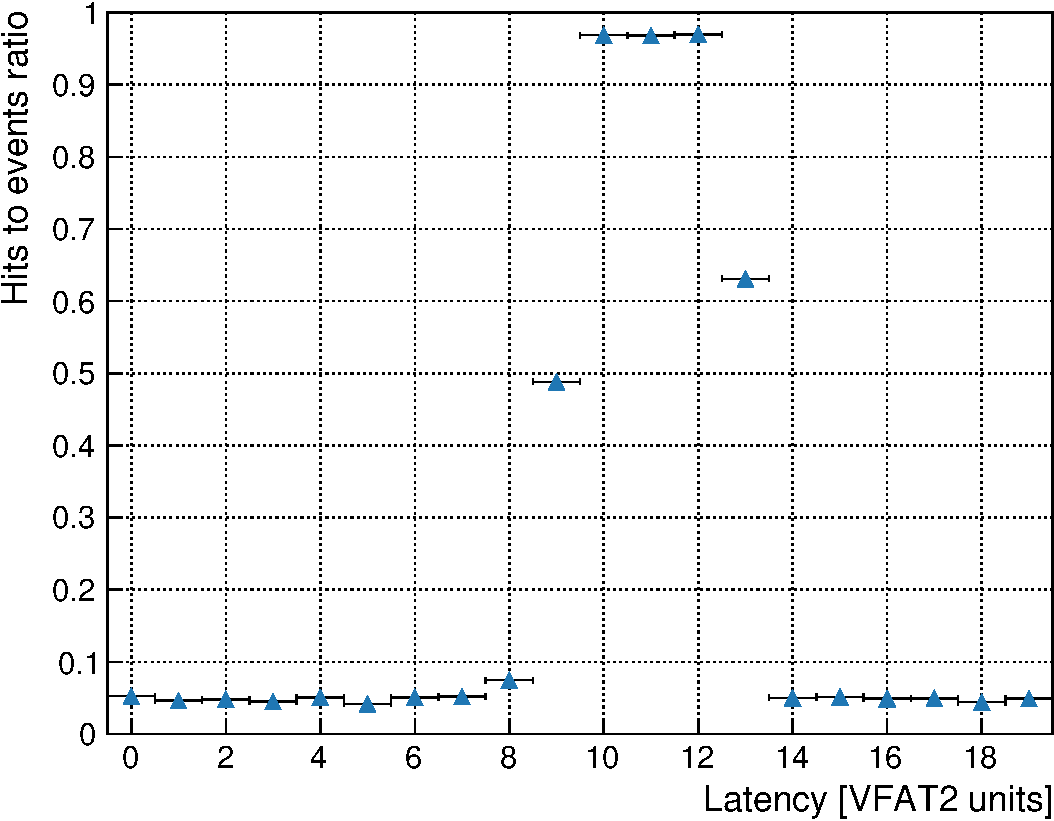
\includegraphics[width=0.49\textwidth]{img/plots/cLatency_GEM0-crop}
        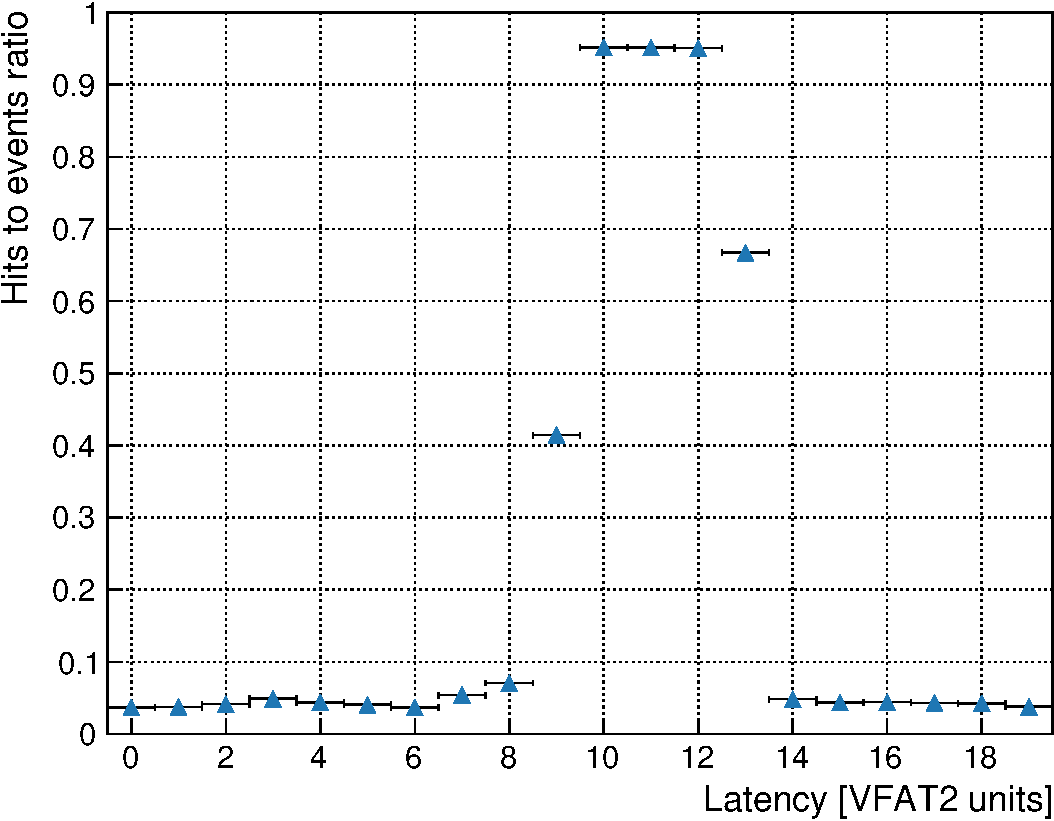
\includegraphics[width=0.49\textwidth]{img/plots/cLatency_GEM1-crop}
        \caption{Plots of the ratio of hit events as a function of the VFAT2 latency in terms of BXs for a monostable pulse length of four clock cycles for GEM0 on the left and GEM1 on the right with muons.}
        \label{fig:II-3-data-latency}
      \end{figure}

      Latency scans are also used to measure the noise and the efficiency of the detector. When looking at out-of-time events, the only contribution to the hits is noise. On the other hand, when considering the window in which the latency is well adjusted, both the noise and the particle hits play a role in the measurement. Taking this value to be the measured efficiency, it corresponds to the ratio between the number of events detected by the GEM detector and those detected by the scintillator system. However, the measured efficiency is the superposition of two Poisson processes: the noise and the real detector efficiency. In order to obtain the computed or real efficiency, simulations were developed to compute upper and lower limits on the real efficiency according to the noise levels. This was achieved by running a thousand pseudo-experiments for each possible efficiency value and comparing the result to the measured value. With a noise level of 100\%, the real efficiency could be anything between 0\% and 100\%. However, with a noise level of 1\%, the computed efficiency will be close to the measured efficiency. For example, for a measured efficiency of 95\% and noise levels of 50\% and 20\%, the resulting computed efficiency is within a range of 89\% - 91\% and 93\% - 94\% respectively. When the noise is lower, the computed efficiency is close to the measured value as the probability of noise faking a hit is less.

    \subsection{Evolution of the Efficiency with the High-Voltage}

      Using the latency scan to compute noise and efficiency values, the evolution of these parameters has been studied according to the high-voltage applied on the detector. Figure \ref{fig:II-3-data-eff-hv} plots the measured noise (green), measured efficiency (blue), and computed efficiency (orange) as a function of the high-voltage expressed in microamperes for GEM0 on the left and GEM1 on the right with muons. Both results show an increase in efficiency with the high-voltage, reaching the start of a plateau around 97\%. This is caused by the higher gain at which the GEM foils start to operate which in turn amplifies the signals and allows it to be detected by the VFAT2 ASIC. It can be noted that a shift exists between the results for GEM0 and GEM1. Values for the latter are shifted to the left by approximately 10 $\mu$A. While GEM0 reaches a plateau at 800 $\mu$A, GEM1 requires 810 $\mu$A to reach an efficiency around 97\%. This is due to the leakage current observed during installation which decreases the voltage applied to the GEM foils and in turn performance. It can also be noted that the noise is constant with the high-voltage and remains at 4\%. From this, it was decided to operate both chambers at 800 $\mu$A as sparks were sometimes observed at 810 $\mu$A. This value is considered to be the default high-voltage except if otherwise specified. \\

      \begin{figure}[b!]
        \centering
        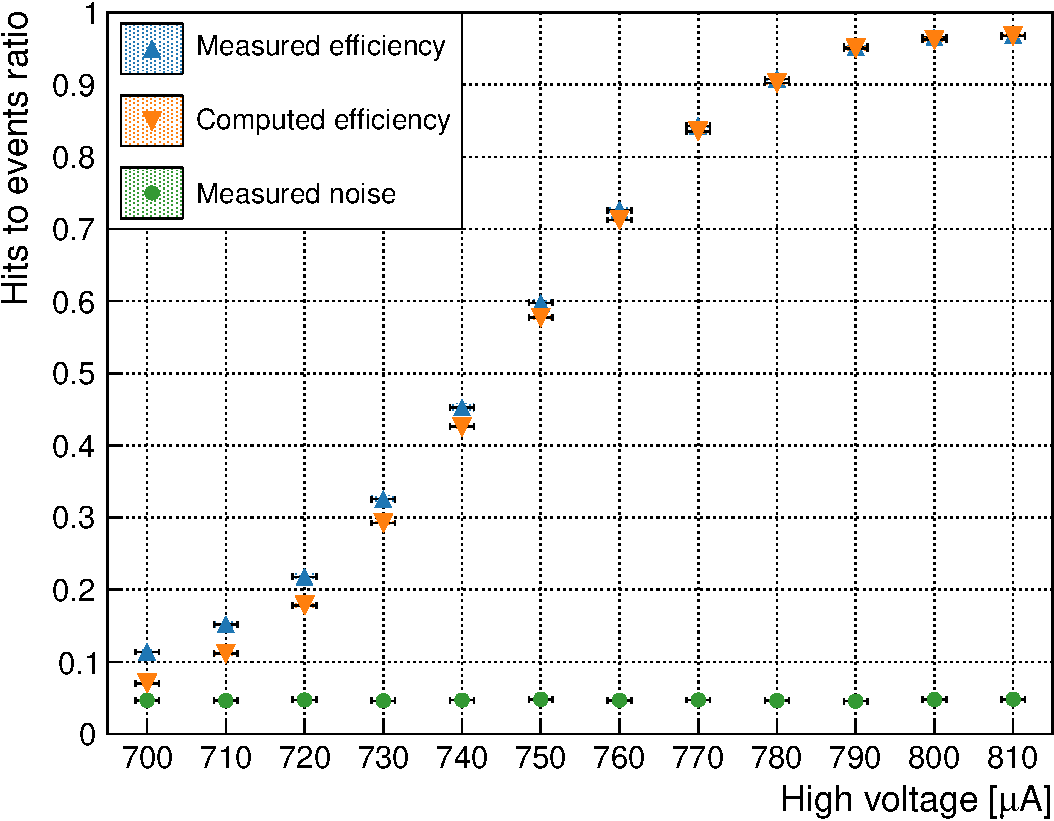
\includegraphics[width=0.49\textwidth]{img/plots/cEfficiency_HV_GEM0-crop}
        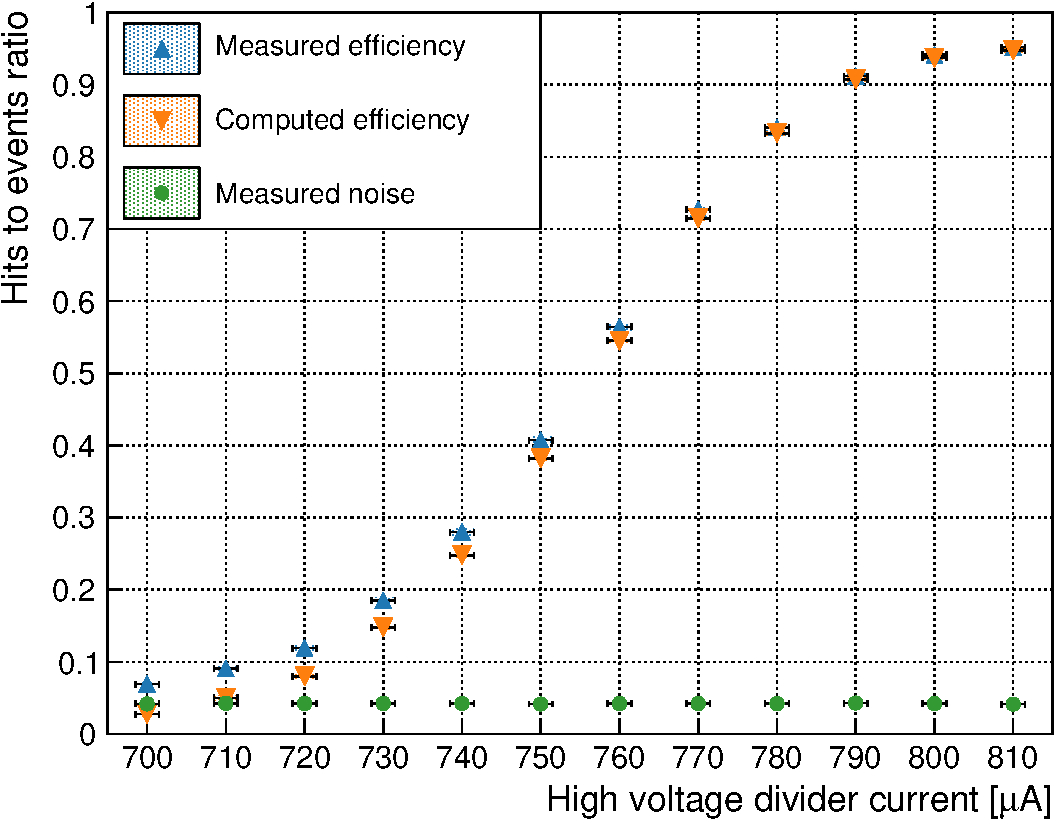
\includegraphics[width=0.49\textwidth]{img/plots/cEfficiency_HV_GEM1-crop}
        \caption{Plots of the measured noise (green), measured efficiency (blue), and computed efficiency (orange) as a function of the high-voltage expressed in $\mu$A for GEM0 on the left and GEM1 on the right with muons.}
        \label{fig:II-3-data-eff-hv}
      \end{figure}

      The results obtained with GEM0 can be compared against the scans performed during previous test beams \cite{Abbaneo:1709907, Abbaneo:1401079} which used the same gas mixture. These scans show the efficiency in terms of gain, which is then expressed in terms of current through the high voltage divider. In the 700 $\mu$A to 810 $\mu$A range, gains of 100 to 8 000 are obtained. Between these values, the efficiency quickly rises to 97\% to reach the very beginning of the plateau. The same behavior is observed in the results exposed here-above. To convert the high voltage from microamperes to a gain, Figure \ref{fig:II-3-gain} is used. The latter yields a range for the gain of 500 to 10 000 in which the efficiency reaches its maximum at the highest values, right at the beginning of the plateau region. A third test beam \cite{Abbaneo:1494965} provides measurements of the efficiency as a function of the high voltage for lower thresholds of 10, 15, and 20. While they reach the efficiency plateau at lower currents, it sits at a value of 95\%, compared to 97\% for the results showed here-above.

    \subsection{Evolution of the Efficiency with the VFAT2 Threshold}

      Although it had been decided to run the system with a VFAT2 threshold of 25, a study of the evolution of the noise and efficiency according to the threshold was performed. It aimed at quantifying the amount of noise and signal that was cut when increasing its value allowing to select the configuration yielding the best signal over noise ratio. This procedure uses tracking data and the full granularity information to analyze events. Figure \ref{fig:II-3-data-eff-threshold} plots the measured noise (green), measured efficiency (blue), and computed efficiency (orange) as a function of the VFAT2 threshold in terms of VFAT2 units for GEM0 on the left and GEM1 on the right with muons. Additional points in purple have been extracted from the tracking data. Using the two GEM detectors, it is possible to measure the efficiency of one using the other as reference. For each event, the following cuts were applied on the GEM of reference in order to reduce the dataset:
      \begin{itemize}
        \item only one cluster, group of adjacent channels that have been hit, is present in the event;
        \item the sole cluster must contain exactly two active channels;
        \item the center of the cluster must be at least ten channels away from the sides of the chip.
      \end{itemize}
      The first condition eliminates events where a hit is accompanied by noise, creating an ambiguity on the cluster associated with the particles. The second condition helps to remove noise related events as they have a cluster size distribution peaked at one channel. Therefore, combining these two criteria creates a stringent condition for the selection of signals generated by particles. The final condition ensures that the hit in the second GEM detector will be located inside the VFAT2 thus eliminating acceptance problems. Using the reduced dataset, the algorithm computed the efficiency by looking for hits in the second GEM detector in a window of ten channels around the center of the cluster of the GEM of reference, which corresponds to a windows of 40 mm. \\

      \begin{figure}[t!]
        \centering
        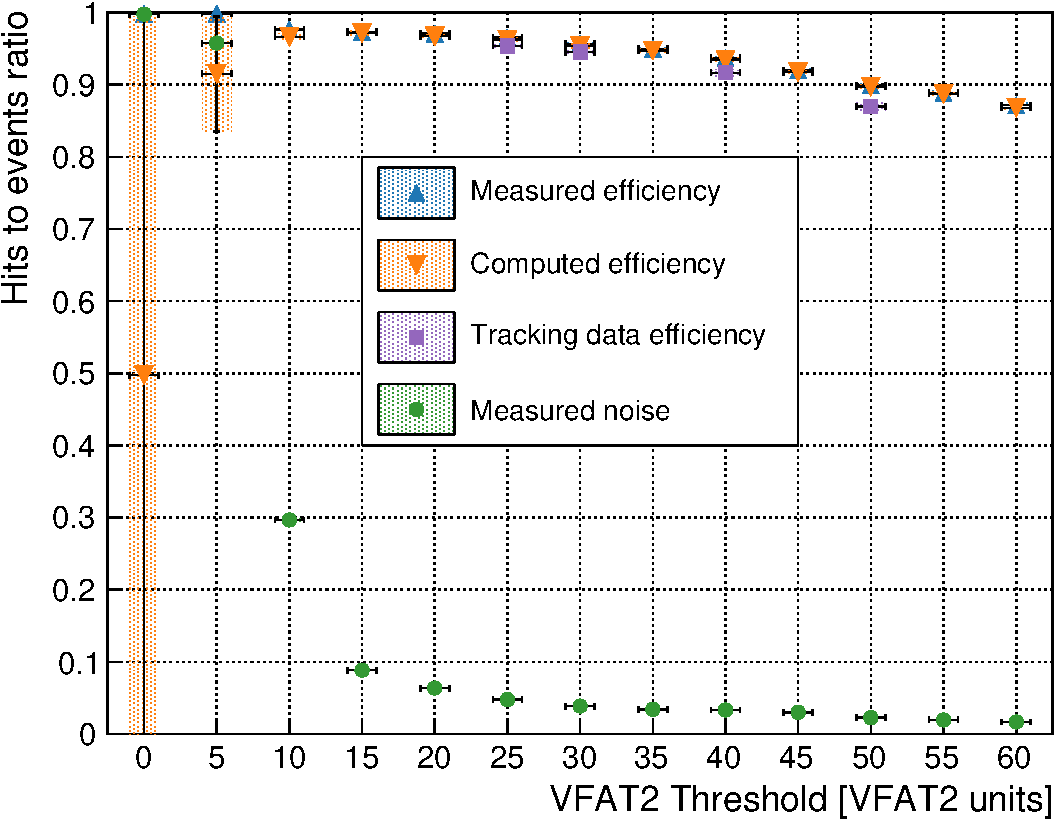
\includegraphics[width=0.49\textwidth]{img/plots/cEfficiency_Threshold_GEM0-crop}
        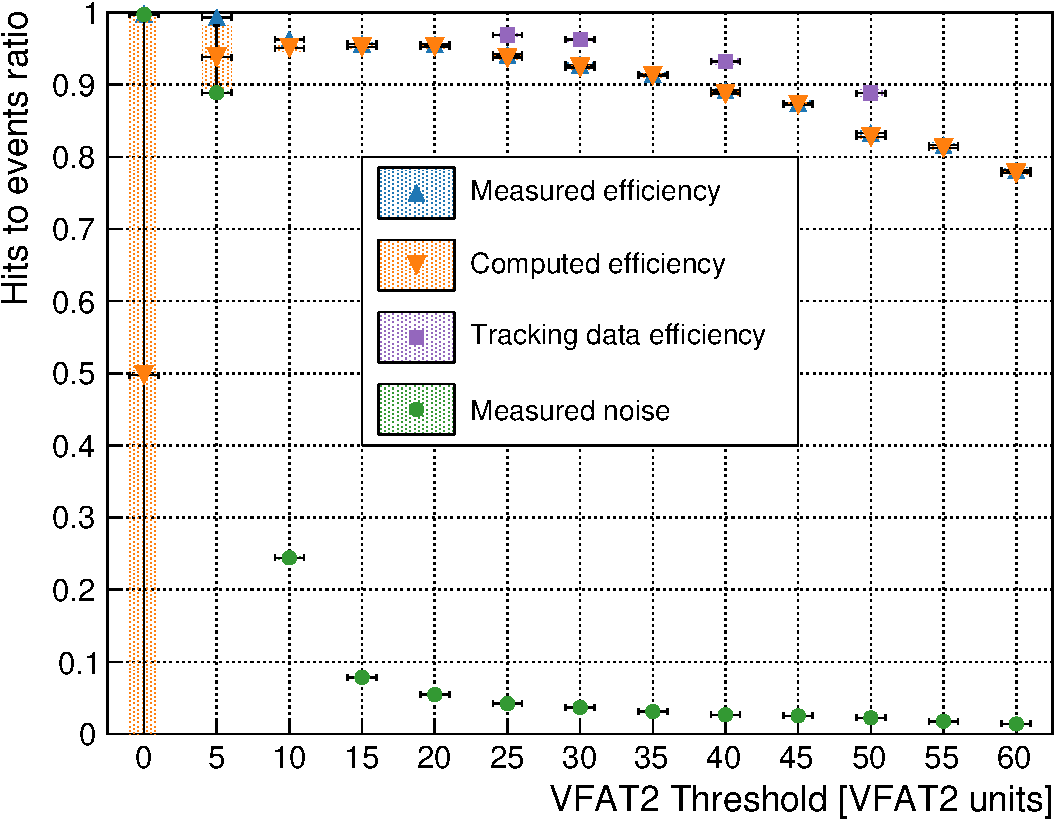
\includegraphics[width=0.49\textwidth]{img/plots/cEfficiency_Threshold_GEM1-crop}
        \caption{Plots of the measured noise (green), measured efficiency (blue), computed efficiency (orange), and tracking data based efficiency (purple) as a function of the VFAT2 threshold in terms of VFAT2 units for GEM0 on the left and GEM1 on the right with muons.}
        \label{fig:II-3-data-eff-threshold}
      \end{figure}

      It can be noted that at very low thresholds the computed efficiency displays a large error due to the high noise. As the latter decreases with the increase in the threshold, the algorithm computing the real efficiency is able to tighten its limits ultimately providing a computed efficiency close to the measured value. From a threshold value of 15, efficiency starts to slowly drop from 98\% to 90\% at 50. This shows how the threshold cuts the signal while only slightly affecting noise which remains at 4\% at thresholds above 25. From these results, the choice to operate the system at a threshold of 25 is validated. Although displaying a slightly lower efficiency, still around 97\%, than results at a threshold of 15, the lower noise is non-negligible and reaches a local plateau. The deviation between the efficiency obtained using the latency scans and the tracking data for GEM1 comes from the higher noise to which it is subject. Apart from the requirement that the hits in GEM1 should be within a given windows around the hit in GEM0, no other cut is performed on the data in order to not bias the results. Therefore, the higher noise in GEM1 will artificially increase the efficiency when faking a hit.

    \subsection{Evolution of the Efficiency with the Trigger Rate}

      Similarly to the measurements and computations made for the previous study, the effect of trigger rate on the efficiency was measured. Focus is given on the latter as the noise levels are not influenced by the increase in rate and remain at 4\%. Figure \ref{fig:II-3-data-eff-rate} plots the measured efficiency (blue), computed efficiency (orange), and tracking data based efficiency (purple) as a function of the trigger rates for GEM0 on the left and GEM1 on the right with pions. The trigger rate was adjusted using collimaters placed in front of the beam setup. As noted in the results shown in the previous section, the deviation between the efficiency obtained using the latency scans and the tracking data for GEM1 comes from the higher noise to which it was subject. \\

      \begin{figure}[t!]
        \centering
        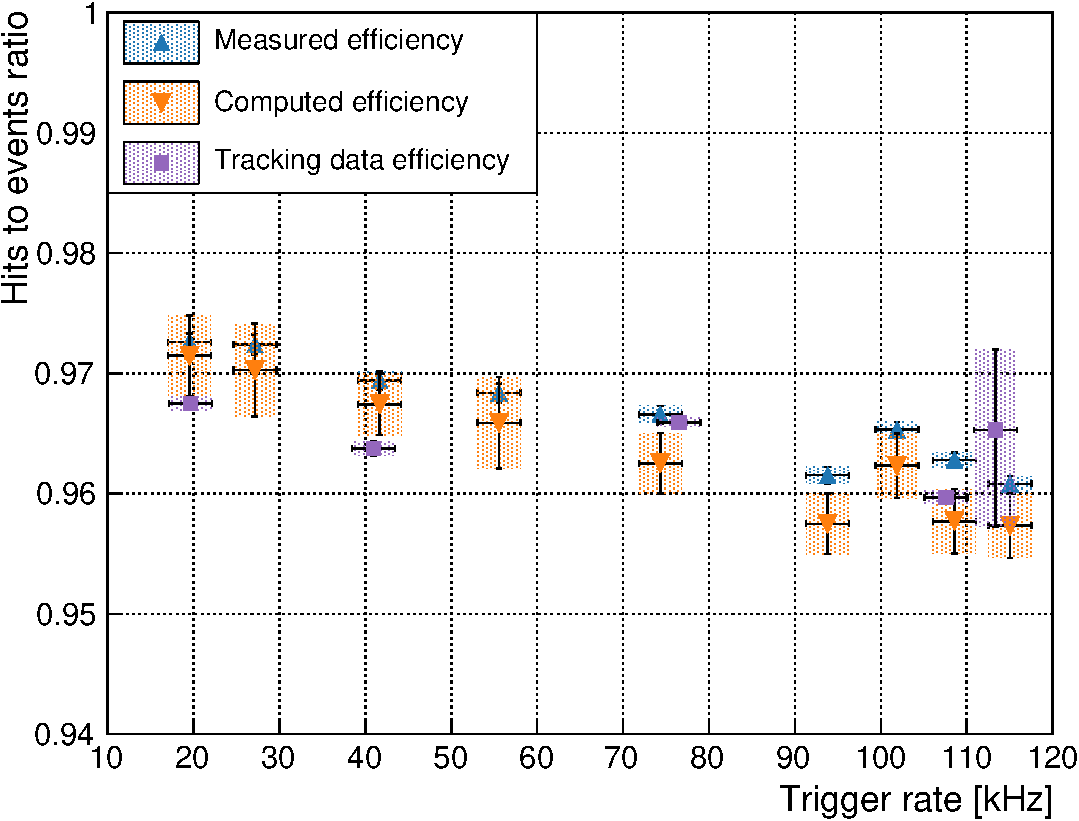
\includegraphics[width=0.49\textwidth]{img/plots/cEfficiency_Rate_GEM0-crop}
        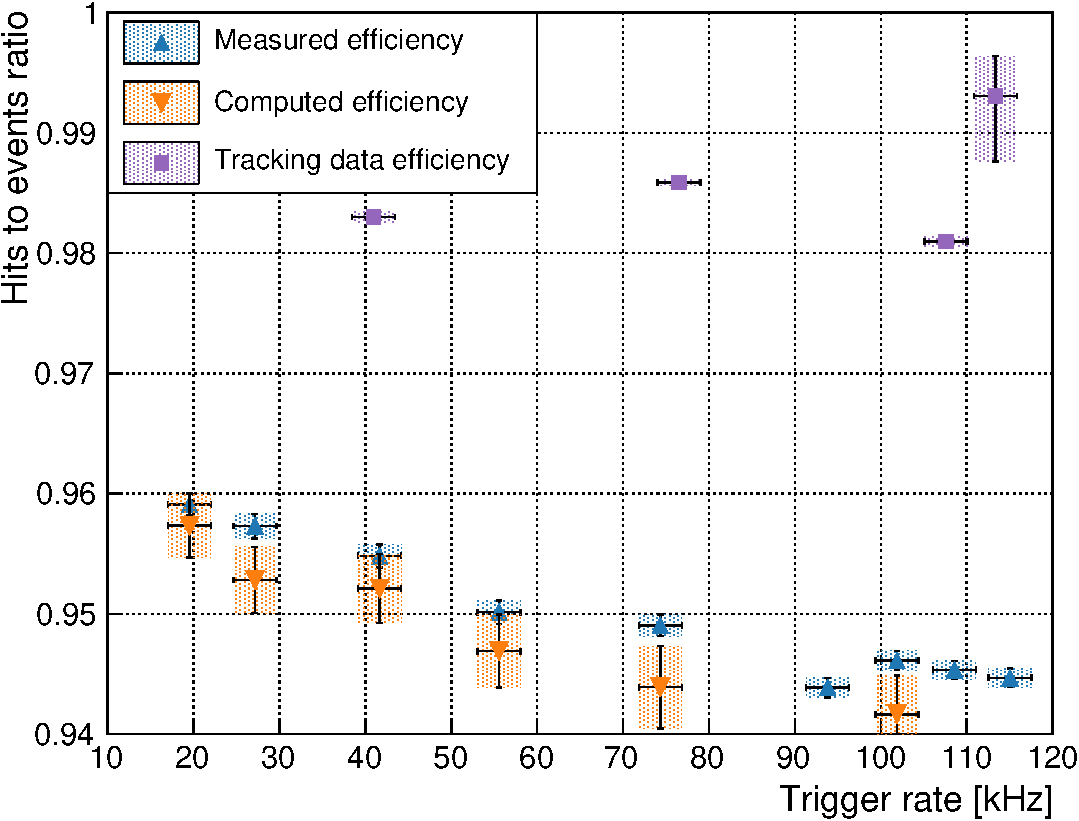
\includegraphics[width=0.49\textwidth]{img/plots/cEfficiency_Rate_GEM1-crop}
        \caption{Plots of the measured efficiency (blue), computed efficiency (orange), and tracking data based efficiency (purple) as a function of the trigger rates for GEM0 on the left and GEM1 on the right with pions.}
        \label{fig:II-3-data-eff-rate}
      \end{figure}

      A small decrease in efficiency of 1\% for GEM0 and of roughly 2\% for GEM1 from the initial value of 97\% is observed When increasing the trigger rate from 20 kHz to 120 kHz. This is due to the charge-up effect that occurs inside the detector \cite{Alfonsi20126}. The electrons and ions created during the avalanche process inside the GEM foils can be absorbed by the Kapton insulator and in turn modify the transparency of the GEM foils. The transparency is defined as the ratio of primary electrons that initiate an avalanche and thus contribute to the formation of the signal, and the total number of primary electrons. Figure \ref{fig:II-3-charge-up} illustrates the drift path (without diffusion) of electrons (orange) starting 90 $\mu$m above the GEM, in an electrostatic configuration (green) without charges on the Kapton surface on the left and with charges on the Kapton surface on the right. As can be seen in the right plot, a significant number of electrons are captured by the coper layer on top of the Kapton when the latter has accumulated charge, thus reducing the transparancy of the foil. This in turn lowers the amplitude of the signal formed on the readout strips \cite{1748-0221-7-01-C01005} and increases the probability that the signal is bellow threshold, meaning the hit is not recorded by the VFAT2. When the counting rate in the chamber is small, the accumulated charge can dissipate, effectively eliminating this effect. \\

      \begin{figure}[t!]
        \centering
        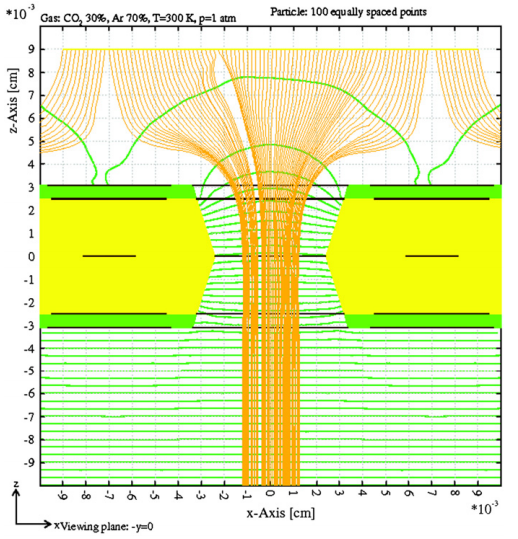
\includegraphics[width=0.49\textwidth]{img/II-3-test-beam/chargeup-0.png}
        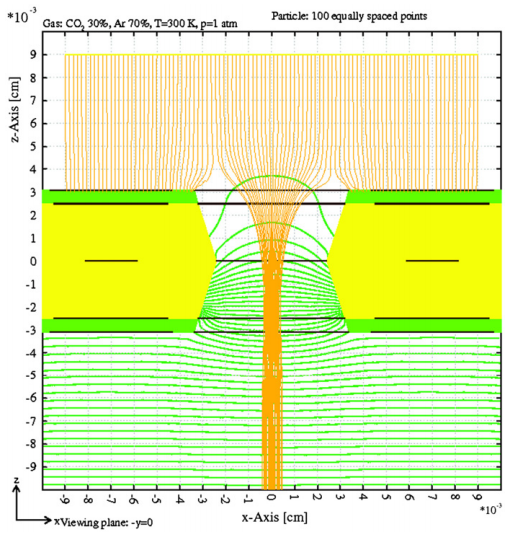
\includegraphics[width=0.49\textwidth]{img/II-3-test-beam/chargeup-1.png}
        \caption{Drift path (without diffusion) of electrons (orange) starting 90 $\mu$m above the GEM, in an electrostatic configuration (green) without charges on the Kapton surface on the left and with charges on the Kapton surface on the right \cite{Alfonsi20126}.}
        \label{fig:II-3-charge-up}
      \end{figure}


      To corroborate the statement that the loss in efficiency originates from the detector and not the DAQ system, the latter has been tested against trigger rates of 200 kHz, the maximum rate supported by the VFAT2s. By providing a know number of triggers to the system and counting the number of data packets read out, it was shown that no data losses occur in the readout chain. These results support the claim that the GEM chamber and DAQ system can sustain trigger rate of CMS, which is of 100 kHz for the LHC Phase I, while keeping an efficiency above 96\%. Finally, it is important to emphasize that the measurements of the efficiency against the threshold show that when lowering the working threshold of the VFAT2s to 15 instead of 25, the efficiency increases by 1\% to 2\%. This means a final efficiency above 97\% could be achieve.

    \subsection{Cluster Multiplicity and Size}

      Two studies that can be performed offline using the recorded data are the evolution of the cluster multiplicity, the number of clusters, and the cluster size, the number of channels per cluster, with the VFAT2 threshold. Figures \ref{fig:II-3-data-clu-mult} and \ref{fig:II-3-data-clu-size} respectively plot the cluster multiplicity and cluster size for muons (green) and pions (blue) as a function of the VFAT2 threshold in terms of VFAT2 units for GEM0 on the left and GEM1 on the right. \\

      \begin{figure}[b!]
        \centering
        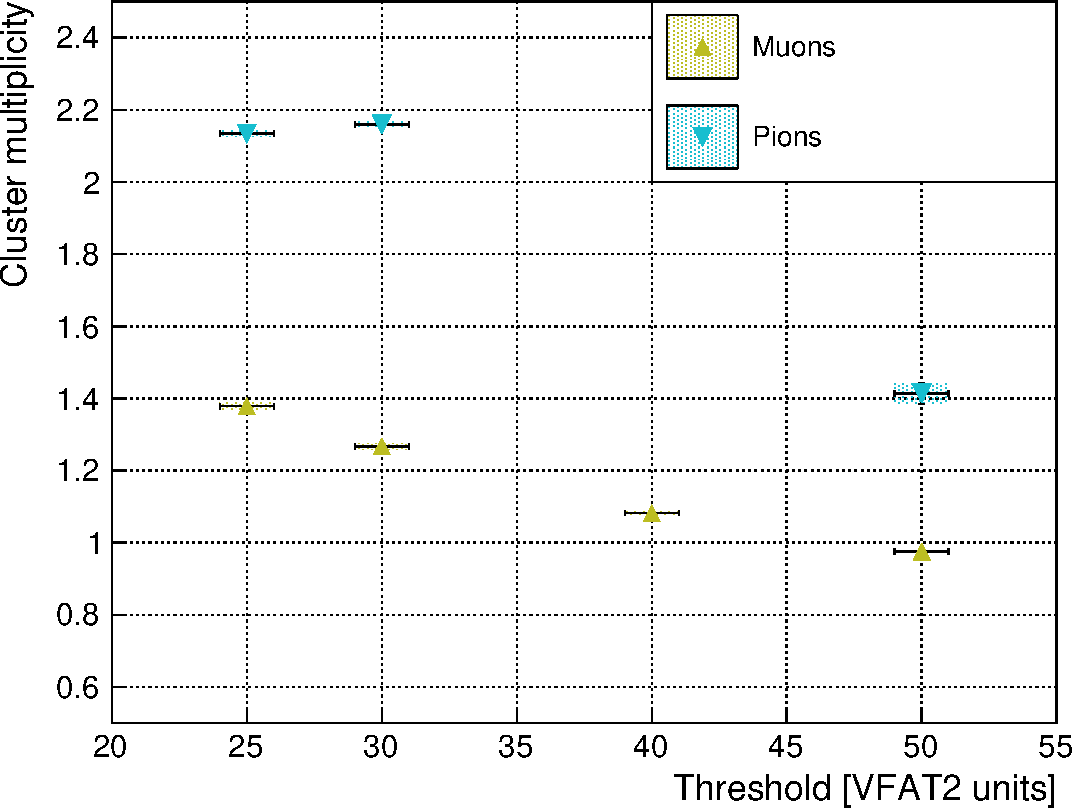
\includegraphics[width=0.49\textwidth]{img/plots/cClusterMultiplicity_Threshold_GEM0-crop}
        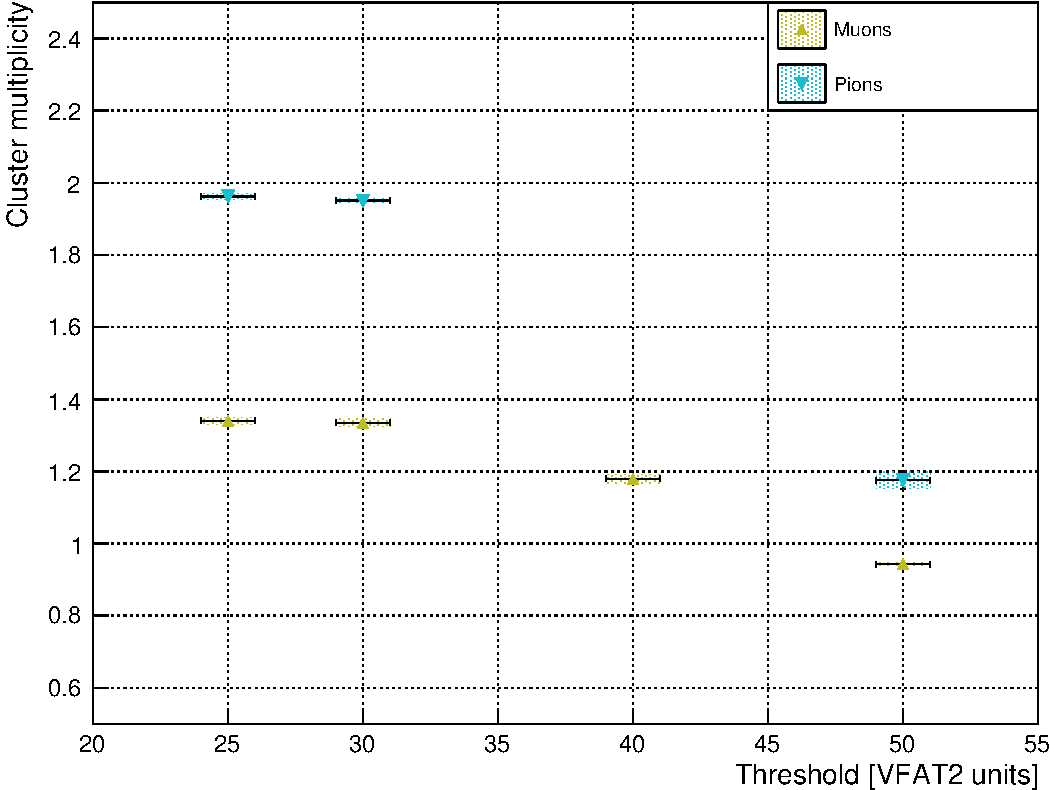
\includegraphics[width=0.49\textwidth]{img/plots/cClusterMultiplicity_Threshold_GEM1-crop}
        \caption{Plots of the cluster multiplicity for muons (green) and pions (blue) as a function of the VFAT2 threshold in terms of VFAT2 units for GEM0 on the left and GEM1 on the right.}
        \label{fig:II-3-data-clu-mult}
      \end{figure}

      The cluster multiplicity reflects the number of clusters present in the event, some of which are due to noise, others to signal. Its evolution is tightly linked to the evolution of the efficiency as a function of the VFAT2 threshold. It was observed that for threshold values of 25 and 30, the noise and efficiency were only slightly decreasing and remained at 4\% and 97\% respectively. At a higher threshold of 50 VFAT2 units however, the efficiency dropped to 90\%. This explains that the points at 25 and 30 for both pions and muons in GEM0 and GEM1 have similar values ($\pm$ 0.1). When the threshold is further increased to 50, the effects start to appear, cutting the signal and removing clusters. \\

      The impact of the efficiency according to the threshold is however not directly visible when considering the cluster size. It is clear that the cluster size decreases as the threshold increases, meaning that less and less channels are being fired. At low threshold, clusters contain roughly 1.5 channels and an average of 1.6 clusters are present per event. When increasing the threshold, the average number of channels fired decreases slightly which does not immediately affect the cluster multiplicity: clusters are reduced in size but not in numbers. The counting of cluster is not directly affected by the cluster size when the latter is greater than one. This means that two clusters of size two are equivalent to two clusters of size one. Even if by increasing the threshold, some channels are being deactivated, other channels in the cluster might still remain active thus leaving the cluster statistic unchanged. \\

      \begin{figure}[b!]
        \centering
        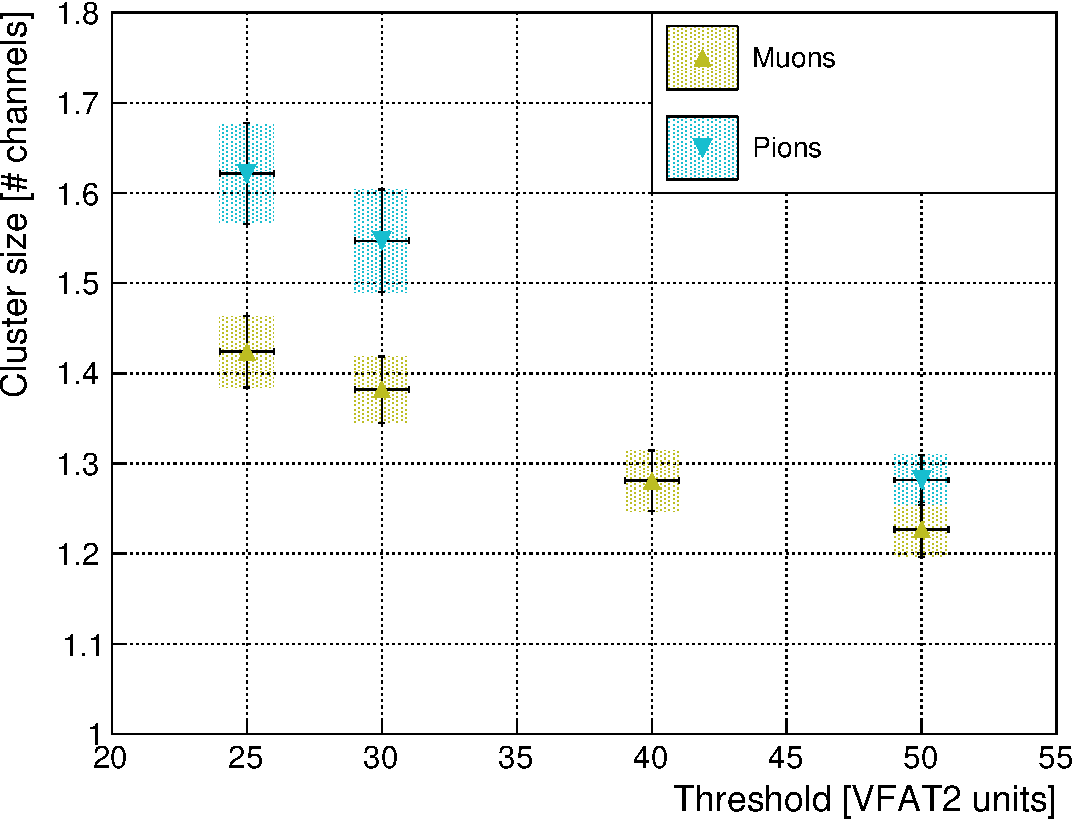
\includegraphics[width=0.49\textwidth]{img/plots/cClusterSize_Threshold_GEM0-crop}
        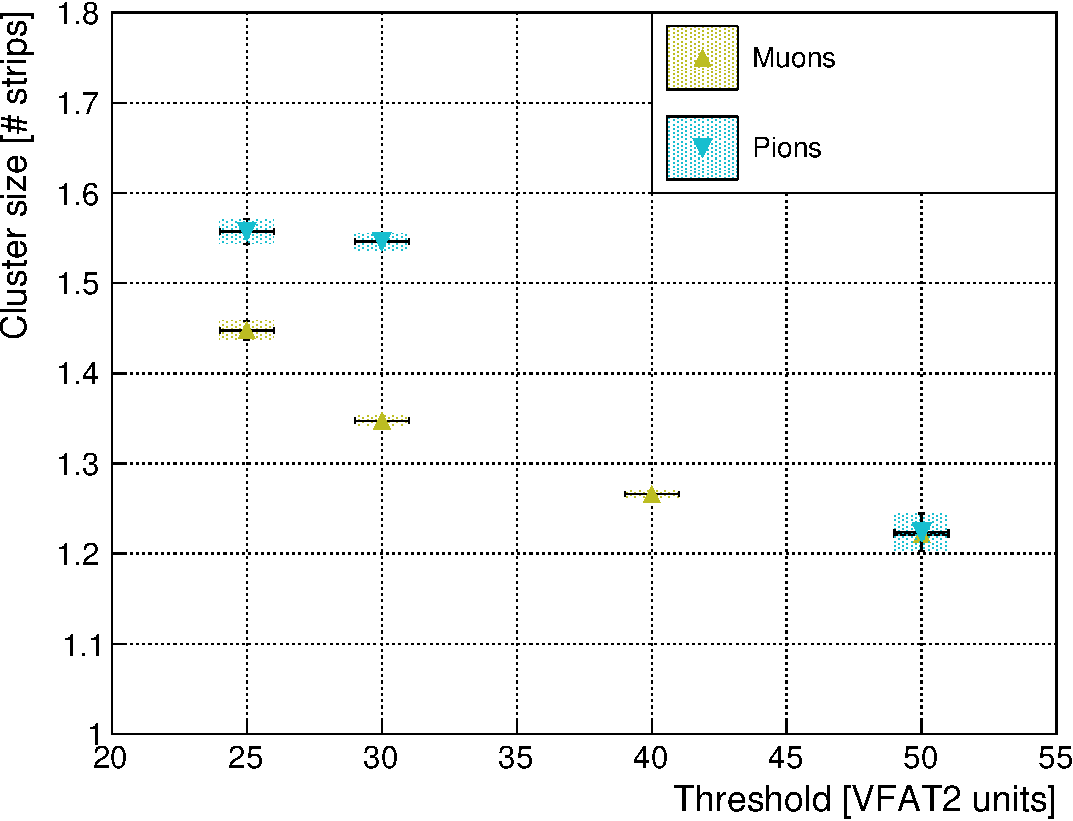
\includegraphics[width=0.49\textwidth]{img/plots/cClusterSize_Threshold_GEM1-crop}
        \caption{Plots of the cluster size for muons (green) and pions (blue) as a function of the VFAT2 threshold in terms of VFAT2 units for GEM0 on the left and GEM1 on the right.}
        \label{fig:II-3-data-clu-size}
      \end{figure}

      Two test beam campaigns \cite{Abbaneo:1401079, Abbaneo:1494965} studied the distribution of the cluster size and provide a reference point against which the results here-above can be compared. These tests respectively yielded an average cluster size of 1.79 $\pm$ 1.16 for a mixed muon/pion beam at a threshold of 20 VFAT2 units, and 1.75 (no errors given) for a muon beam at a threshold of 12 VFAT2 units. The first measurement did not distinguish data taken during muon and pion runs and is thus an average of the two. Performing the same operation on the results shown above and assuming an equal number of events for both types of particles, an average value of 1.57 $\pm$ 1.1 is obtained. In order to compare the data against the second set of results, a quadratic extrapolation of the data points for the muons shown in the left plot of Figure \ref{fig:II-3-data-clu-size} was done towards 12 VFAT2 units. The obtained cluster size is of 1.77 $\pm$ 0.4. In both cases, the cluster sizes obtained during the previous test beams and the results shown above are well within the error bars and show excellent agreement. Additional measurements have been performed in previous studies \cite{Abbaneo:1973272} at Fermilab using hadron beams. These yielded a cluster size greater than for muon beams at a value of 2.43 $\pm$ 1.04, which is also visible in the results above. \\

      These results confirm the different behaviors between muons and pions: the former with a cluster size around 1.42 $\pm$ 0.5, and the latter around 1.62 $\pm$ 0.6. This originates from the higher interaction rate of the pion beam with the material placed in front of the GEM detectors, which causes the creation of secondary particles. As the beam is collimated and hits around 40 channels on the VFAT2, the clusters resulting from different particles overlap and artificially increase the cluster size. When clusters do not overlap, it is the cluster multiplicity which is increased.

    \subsection{Beam Profile}

      Finally, to illustrate the structure of the beam, one can create a beam profile obtained by superimposing the collected data and counting the number of hits for each channels. Figure \ref{fig:II-3-data-beam-profile} plots the beam profile for muons (green) and pions (blue) for GEM0 on the left and GEM1 on the right. The pion beam is well defined and centered on the VFAT2 as it is guided and collimated by the magnets of the transfer tunnels from the SPS to the experimental area. The muon beam on the other side displays a large spread due to the decay process of the pions and the collimators installed to stop them. The sharp cut-off on the left side of the profile is due to the geometrical acceptance of the PM placed in the back of the detector. These plots show that the chips do not have any dead channels.

      \begin{figure}[b!]
        \centering
        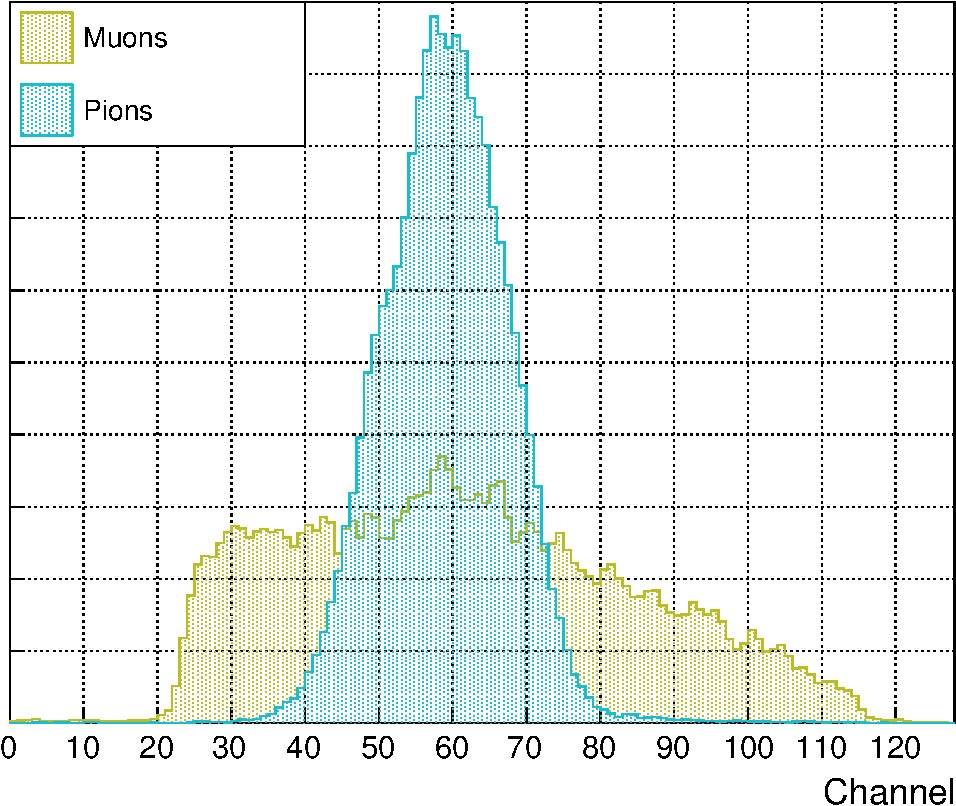
\includegraphics[width=0.49\textwidth]{img/plots/cBeamProfile_GEM0-crop}
        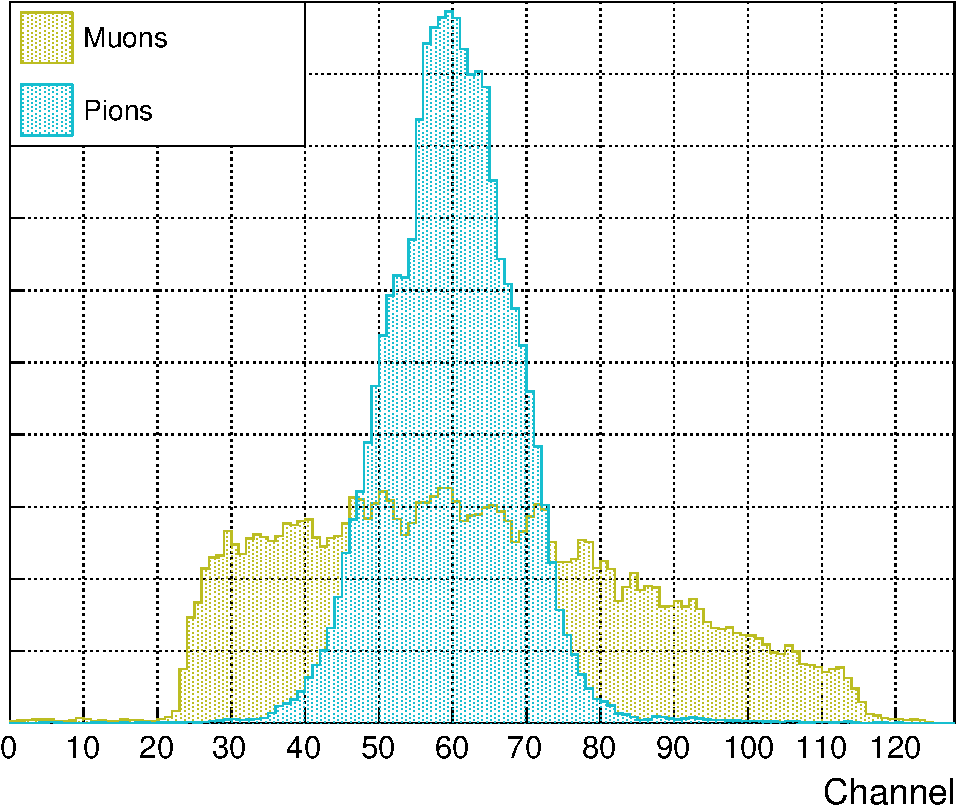
\includegraphics[width=0.49\textwidth]{img/plots/cBeamProfile_GEM1-crop}
        \caption{Plots of the beam profile for muons (green) and pions (blue) for GEM0 on the left and GEM1 on the right.}
        \label{fig:II-3-data-beam-profile}
      \end{figure}

  \section{Towards the Slice Test}

    Using the feedback obtained during the test beam, a OptoHybrid v2b was designed which incorporated the GBT chipsets (see Section \ref{sec:II-2-gbt}). In addition to porting the code to the new board, firmware developments were required in order to make use of the latter and move from the GTX and SFP+ optical links to the GBT chipset coupled with the Versatile Link. The resources available in the FPGA and the flexibility of the Wishbone bus allowed for the two technologies to be implemented and control the system at the same time. This increases redundancy and offers the possibility to switch between the GTX and GBT in case of failure. \\

    The GBT chipset is connected to the OptoHybrid through two E-Links for the receiver and four E-Links for the transmitter, all running at 320 MHz. This configuration allows to receive 16 bits and transmit 32 bits per BX. The asymmetry is due to the requirement of a higher bandwidth for the link to the off-detector electronics which carries the slow control and tracking data. \\

    On the FPGA, the data is deserialized and aligned using a communication protocol ran during a synchronization phase between the OptoHybrid and the CTP7. As the 40 MHz clock on the former is generated from the 320 MHz clock, the phase relation with the clock of the latter is not known which causes data to be misaligned. At start up, the CTP7 sends a constant pattern of 0x76BC which the OptoHybrid tries to find in the data. If the pattern is not found, a bitslip is operated, shifting the received data by one unit. The operation is repeated until the link is aligned. At that moment, the OptoHybrid, which was transmitting a stream of zeros, switches to a constant pattern of 0x76BC76BC. When the CTP7 is able to identify this pattern, it returns a single 0x8943 word informing the OptoHybrid that data is aligned. Otherwise, the latter performs a bitslip on the transmitted data. \\

    Once the alignment procedure is done, the two systems can communicate through the data format exposed in Table \ref{tab:II-3-gbt-format}. Although similar to the data format used over the GTX links, two fundamental changes have been operated: due to the fact that data is clocked at 40 MHz in the fabric of the FPGA, the TTC commands need to be sent every BX; the bandwidth has been changed modifying the width of the data packets. \\

    \begin{table}
      \begin{tabularx}{\textwidth}{C{1.15}C{0.85}}
        \textbf{CTP7 to OptoHybrid frame} & \textbf{OptoHybrid to CTP7 frame} \\
        {
        \begin{tabularx}{0.52\textwidth}{|C{0.5}|C{1.25}|C{1.25}|}
          \hline
          \multicolumn{3}{|c|}{15 \hfill 0} \\ \hline
          TTC & Header[3:0] & Address[31:24] \\ \hline
          TTC & \multicolumn{2}{|c|}{Address[23:12]} \\ \hline
          TTC & \multicolumn{2}{|c|}{Address[11:0]} \\ \hline
          TTC & 0000 & Data[31:24] \\ \hline
          TTC & \multicolumn{2}{|c|}{Request Data[23:12]} \\ \hline
          TTC & \multicolumn{2}{|c|}{Request Data[11:0]} \\ \hline
          TTC & \multicolumn{2}{|c|}{0xABC} \\ \hline
        \end{tabularx} }
        &
        { \begin{tabularx}{0.4\textwidth}{|C{1}|C{1}|}
          \hline
          \multicolumn{2}{|c|}{31 \hfill 0} \\ \hline
          Header[3:0] & 0x000BCBC \\ \hline
          \multicolumn{2}{|c|}{VFAT2 data x7} \\ \hline
          \multicolumn{2}{|c|}{Response data} \\ \hline
        \end{tabularx} }
      \end{tabularx}
      \caption{Data format of the packets sent between the off-detector and on-detector electronics over the GBT link.}
      \label{tab:II-3-gbt-format}
    \end{table}

    Running along the GTX core, the GBT module is defined as a Wishbone master meaning it can operate the same requests as the former. Furthermore, tracking data is duplicated and sent over the two links ensuring redundancy and protection against failure as the CTP7 can dynamically change between the two cores.

  \section{Towards the Final DAQ System}

    The VFAT2 was designed to handle trigger rates up to 100 kHz and transmit data at a maximum rate of 0.32 Gbps for the trigger data and 0.02 Gbps for the tracking data. These data rates can easily be accommodated by the current system, however, they will be drastically increased for the final system using the VFAT3 ASIC. Furthermore, it is foreseen to multiply the L1A rate by a factor 10 from the current 100 kHz to 1 MHz. It is thus crucial to ensure that the GBT and other components will be able to cope with this increase. \\

    The VFAT3 will output 64 trigger bits per BX which will be collected by the OptoHybrid. Many of these are empty as less than one particle hits the chamber per BX on average. A zero suppressing algorithm is thus implemented on the OptoHybrid in order to only encode bits which are active. Each fired trigger bit requires 11 bits to describe: 5 to address the VFAT3 and 6 to address the strip that is hit. As a maximum of 80 bits per BX can be transmitted over the single 3.2 Gbps data link to the off-detector electronics or the CSCs, the probability that the number of hits exceeds 7 and thus overflows the link can be computed. This results in a probability of less than 6 $ \times $ 10$^{-5}$. To reduce the probability of overflowing the link, double transmitter modules can be used to double the available bandwidth. \\

    The tracking data can be zero suppressed by the VFAT3 itself resulting in data packets of minimum 48 bits compared to the 246 bits when using the lossless data format. Simulations were developed in order to compute the mean size of the data packets while taking into account the rate of particles to which GE1/1 will be exposed. This results in a data rate of 0.17 Gbps and 0.48 Gbps for the zero suppressed and lossless algorithms respectively. Both have a probability of less than 10$^{-7}$ to overflow the three GBT data links. When running at L1A rates of 1 MHz, a factor of 10 is applied to the resulting data rates, which still yield a probability of overflow less than 10$^{-7}$, limit of the simulation.

  \section{Conclusion}

    The November 2015 test beam campaign showed that the DAQ system composed of the VFAT2 ASIC, GEB v2, OptoHybrid v2a, and GLIB was able to run flawlessly during the entirety of the campaigns. The latter was able to handle two GE1/1 detectors with ease while providing quality data which has been used to compute the noise and efficiency on the system as a function of various parameters as well as the cluster multiplicity and size. \\

    The flexible firmware architecture we developed for the OptoHybrid, which provides the user with numerous monitoring and control options, ran for the duration of the test beam and carried out all required tasks: handle the slow control with the VFAT2s, read out tracking data, and monitor the system. The wishbone-like communication protocol implemented in the FPGA allows future developments to be easily integrated and modules to communicate with one another. The firmware of the GLIB and the communication through the optical links have ran smoothly showing no errors on the transmitted data. The readout rate was high enough to prevent the buffer from overflowing and the data taking has shown to be well integrated with the software. The latter, namely a web application that we designed, has been used extensively and is still in use for gain and uniformity studies at CERN. It has proven to be a complete solution to control and monitor the DAQ system allowing users to run all the necessary scans. \\

    Finally, we have analyzed the data recorded during the test beam. Threshold scans have shown an elevated noise level around 4\%, which has since then been understood and solved, forcing us to work at higher threshold values and thus reducing the efficiency by 1\%-2\% to 97\%. Nonetheless, using the latency scans and the tracking data, we performed various studies of the noise and efficiency levels against high-voltage, threshold, and trigger rates. An efficiency of 97\% has been obtained when running at nominal values, and trigger rate capability has been tested up until 120 kHz with a resulting efficiency of 96\%. Studies on the cluster size have yielded an average of 1.42 $\pm$ 0.5 for muons and 1.62 $\pm$ 0.6 for pions. These results are in excellent agreement with measurements performed during two test beams campaigns. \\

    From the analysis we have performed and the results obtained for the efficiency of the system, we conclude that the GEM detectors equipped with the DAQ system we have designed meet the requirements of the project regarding the efficiency and the rate capability of the chambers.
